\chapter{Théorie des ensembles}

\section{Notions de base}

\begin{definition}[: ensemble, éléments]
    Nous nous contenterons de dire qu'un \textit{ensemble} est une \textit{collection d'objets}  appelés \textit{éléments} et qu'on peut clairement dire, lorsqu'on considère un objet, s'il appartient ou non à cet ensemble.\\
    Pour signifier que l'élément $x$ appartient à l'ensemble $E$ on écrit $x\in E$. Pour signifier le contraire on écrit $x\notin E$.
\end{definition}

\begin{exemple}[s]
    \begin{itemize}
        \item
              L'ensemble $\mathcal{J}$ des jours de la semaine peut se noter :
              $$\mathcal{J}=\left\lbrace\ LUN\ ;\ MAR\ ;\ MER\ ;\ JEU\ ;\ VEN\ ;\ SAM\ ;\ DIM\ \right\rbrace$$


        \item 	On note $\N$ l'ensemble de tous les entiers positifs. On a donc $2020\in\N$, mais $3,2\notin\N$.
        \item 	Les solutions dans $\R$ de l'inéquation $x^2<4$ forment un ensemble : $\oio{-2}{2}$.
    \end{itemize}

\end{exemple}
\begin{definition}[s : ensemble vide et singleton]
    \begin{itemize}
        \item 	L'ensemble qui ne contient aucun élément s'appelle \textit{l'ensemble vide} et se note $\emptyset$.
        \item 	Soit $x$ un objet, alors l'ensemble composé de l'unique élément $x$ se note $\lbrace x\rbrace$ et s'appelle un \textit{singleton}.
    \end{itemize}
\end{definition}

\begin{definition}[s : écritures en extension et compréhension]

    Quand un ensemble est \textit{fini} (on reviendra sur cette notion plus tard), on peut donner la liste \textit{exhaustive} de ses éléments comme ceci :\\

    E = $\lbrace $Paris; Marseille; Lyon; Toulouse; Nice; Nantes; Montpellier, Strasbourg, Bordeaux$\rbrace$\\
    L'écriture précédente est appelée \textit{écriture en extension}.\\

    « E est l'ensemble des 9 plus grandes villes de France. » \\
    Lorsqu'on écrit la phrase précédente, on donne une autre manière de définir E : pas par son contenu explicite, mais par une règle que ses éléments vérifient. On parle d'\textit{écriture en compréhension}.
\end{definition}

\begin{exemple}[s]
    \begin{itemize}
        \item 	$E=\lbrace 0;\,1;\;2\rbrace$ est écrit en extension. En compréhension on écrira $E=\lbrace n\in\N,\,n\leq 2\rbrace$.
        \item 	On considère $F=\lbrace n\in\N, n\equiv 2,\,[3]\rbrace$, c'est un ensemble \textit{infini}, on ne peut donc pas écrire la liste de tous ses éléments, mais on peut en donner un « aperçu »  :
              $$F=\left\lbrace 2;\,5;\,8;\,11;\,14;\,...\,\right\rbrace$$
    \end{itemize}
\end{exemple}

\begin{definition}[]
    Quand un ensemble $E$ est \textit{fini}, on appelle \textit{cardinal} de E le nombre de ses éléments, on le note $\card(E)$.
\end{definition}

\begin{remarque}[]
    Un ensemble n'est pas une variable de type \mintinline{python}{list} en \textsc{Python}, ou un tableau de \textsc{Visual Basic}, car il n'y a \textit{a priori} pas d'ordre sur les éléments de l'ensemble.\\
    Ainsi l'ensemble $\lbrace \text{ crayon ; stylo }\rbrace$ est le même que l'ensemble $\lbrace \text{ stylo ; crayon }\rbrace$.\\
    En revanche en \textsc{Python}, on a \mintinline{python}{['stylo', 'crayon']} et \mintinline{python}{['crayon', 'stylo']} sont deux listes différentes.


\end{remarque}

\begin{definition}[ : inclusion]
    Soit $A$ et $B$ deux ensembles. Si tout élément de $A$ est également un élément de $B$ alors on dit que \textit{$A$ est inclus dans $B$}.\\
    On écrit alors $A\subset B$ et cela revient à écrire : $\forall x\in A,\,x\in B$.
\end{definition}

\begin{exemple}[s]
    \begin{itemize}
        \item 	En reprenant un exemple précédent on a :
              $$\lbrace \text{ LUN ; JEU ; VEN }\rbrace \subset \mathcal{J}$$
        \item 	Notons $A$ l'ensemble des élèves de la classe et $B$ l'ensemble des élèves de la classe qui habitent Saint-Brieuc.\\
              \begin{center}
                  \begin{tikzpicture}
                      \draw[fill = UGLiBlue,opacity = .3](0,0) ellipse (2 and 4/3);
                      \draw[fill = UGLiPurple,opacity = .3](.5,0) ellipse (1 and 2/3);
                      \draw (-1,0) node{$A$};
                      \draw (1,0) node{ $B$};
                  \end{tikzpicture}

                  $B\subset A$
              \end{center}
    \end{itemize}
\end{exemple}
\begin{remarque}[s]
    \begin{itemize}
        \item Quel que soit l'ensemble $E$, on a $E\subset E$ car la proposition $\forall x\in E,\,x\in E$ est vraie.
        \item 	Quel que soit l'ensemble $A$, $\emptyset \subset A$ : en effet la proposition suivante est vraie : $\forall x\in\emptyset,\,x\in A$.\\
              Cela peut paraître abusif étant donné qu'il n'y a aucun élément dans $\emptyset$. Faisons alors appel à nos cours de logique et montrons que la proposition contraire est fausse, ce qui revient au même. Cette proposition contraire s'énonce :\\
              $\exists\, x\in\emptyset,\,x\notin A$. Elle est évidemment fausse puisqu'on ne peut trouver $x\in\emptyset$.
        \item 	Il n'existe pas d'\textit{ensemble de tous les ensembles} : on ne peut pas se dire que les ensembles peuvent tous être rangés dans un « gros ensemble » . En revanche (et c'est ce qu'on va faire), il est possible de se donner un ensemble de départ $E$ et de considérer tous les ensembles inclus dedans.
    \end{itemize}
\end{remarque}
\section{L'algèbre de Boole des parties d'un ensemble}
\begin{definition}[ : ensemble des parties d'un ensemble]
    On se donne un ensemble $E$. L'ensemble de \textit{tous les ensembles inclus dans } $E$ se note $\mathcal{P}(E)$. On l'appelle aussi \textit{ensemble des parties de $E$}.
    \begin{itemize}
        \item 	On a vu que $\emptyset\subset E$, ce qui se réécrit $\emptyset\in\mathcal{P}(E)$.
        \item 	De même $E\subset E$, ce qui se réécrit $E\in\mathcal{P}(E)$.
    \end{itemize}
\end{definition}
\begin{exemple}[]
    Posons $E=\lbrace a;\,b;\,c\rbrace$ et donnons tous les éléments de $\mathcal{P}(E)$ :
    \begin{itemize}
        \item 	il y a $\emptyset$;
        \item 	il y a $\lbrace a\rbrace$, $\lbrace b\rbrace$ et $\lbrace c\rbrace$;
        \item 	il y a $\lbrace a;\,b\rbrace$, $\lbrace a;\,c\rbrace$ et $\lbrace b;\,c\rbrace$, parties à 2 éléments.
        \item 	il y a $E$ lui même.
    \end{itemize}
    Ainsi $\mathcal{P}(E)=\left\lbrace \emptyset;\,\lbrace a\rbrace ;\,\lbrace b\rbrace ;\,\lbrace c\rbrace ;\,\lbrace a;\,b\rbrace ;\,\lbrace a;\,c\rbrace ;\,\lbrace b;\,c\rbrace ;\,\lbrace a;\,b;\,c\rbrace \right\rbrace$ comporte 8 éléments.
\end{exemple}

\begin{exercice}[]
    Déterminer $\mathcal{P}(E)$ lorsque $E=\lbrace r;\,s;\,t;\,u;\,v\rbrace$.
\end{exercice}
\begin{definition}[ : intersection]
    \begin{center}
        \begin{tikzpicture}
            \draw[fill = UGLiBlue,opacity = .2](0,0) ellipse (2 and 4/3);
            \draw[fill = UGLiPurple,opacity = .2](2,0) ellipse (2 and 4/3);
            \draw (-1,0) node{$A$};
            \draw (3,0) node{$B$};
            \draw (1,0) node{$A\cap B$};
        \end{tikzpicture}
    \end{center}
    Soient $A$ et $B$ deux ensembles. On appelle \textit{intersection} de $A$ et de $B$ et on note $A\cap B$ l'ensemble dont les éléments appartiennent à la
    fois à $A$ et à $B$.
\end{definition}

\begin{definition}[ : union]
    Soient $A$ et $B$ deux ensembles. On appelle \textit{union} de $A$ et de $B$ et on note $A\cup B$ l'ensemble dont les éléments à $A$ ou bien à $B$.\\
    \begin{center}
        \begin{tikzpicture}
            \begin{scope}
                \draw[fill = UGLiBlue!30](0,0) ellipse (2 and 4/3);
                \draw[fill = UGLiBlue!30](2,0) ellipse (2 and 4/3);
                \clip	ellipse (2 and 4/3);
                \draw[fill = UGLiBlue!30, UGLiBlue!30](2,0) ellipse (2 and 4/3);
                \draw[dashed](2,0) ellipse (2 and 4/3);
                \clip (2,0) ellipse (2 and 4/3);
                \draw[fill = UGLiBlue!30, UGLiBlue!30] ellipse (2 and 4/3);
                \draw[dashed] ellipse (2 and 4/3);
            \end{scope}
            \draw (3,0) node{$B$};
            \draw (-1,0) node{$A$};
            \draw (1,-1.6) node{$A\cup B$};
        \end{tikzpicture}
    \end{center}
\end{definition}

\begin{exemple}
    Considérons les ensembles $A=\lbrace \ u\ ;\ v\ ;\ w\ \rbrace$ et $B=\lbrace \ u\ ;\ w\ ;\ x\ ;\ y\ \rbrace$.\\
    Alors \textbf{ $$A\cap B=\lbrace \ u\ ;\ w\ \rbrace$$} et \textbf{ $$A\cup B=\lbrace \ u\ ;\ v\ ;\ w\ ;\ x\ ;\ y\ \rbrace$$}
\end{exemple}
\begin{definition}[ : complémentaire]
    Soit $A$ une partie de E.\\
    On appelle complémentaire de $A$  dans $E$ et on note $\overline{A}$ l'ensemble des éléments de $E$ qui n'appartiennent pas à $A$.
    \begin{center}
        \begin{tikzpicture}
            \draw[fill = UGLiBlue!30](0,0) ellipse (2 and 4/3);
            \draw[fill = white](1,0) ellipse (.9 and 2/3);
            \draw (1,0) node{$A$};
            \draw (-1,0) node{$\overline{A}$};
            \draw (2,0)--(3,0) node[right]{$E$};
        \end{tikzpicture}
    \end{center}
\end{definition}

\begin{exemple}[]
    En prenant $E=\left\lbrace\ LUN\ ;\ MAR\ ;\ MER\ ;\ JEU\ ;\ VEN\ ;\ SAM\ ;\ DIM\ \right\rbrace$ comme ensemble de départ, le complémentaire dans $E$ de $\lbrace  LUN;\, JEU;\, VEN\rbrace$ est $\lbrace  MAR;\, MER;\, SAM;\,DIM\rbrace$.
\end{exemple}
\begin{exercice}[]
    $A$ et $B$ sont deux parties de $E$. Colorier l'ensemble demandé.
    \begin{multicols}{3}
        \begin{enumerate}
            \item 	$A\cup \overline{B}$\\

                  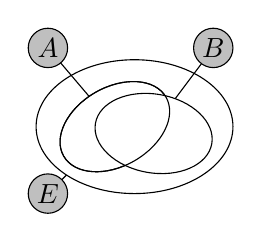
\begin{tikzpicture}[scale=.5]
                      \draw (-1.7,-1.7) -- (0,0);
                      \draw [fill = gray!50](-1.7,-1.7) circle(.5) node{$E$};
                      \draw [fill = white](0.5,0) ellipse (2.5 and 1.7);

                      \draw (-1.7,2) -- (0,0);
                      \draw [fill = gray!50](-1.7,2) circle(.5) node{$A$};
                      \draw [rotate=30,fill = white](0,0) ellipse (1.5 and 1);

                      \draw (2.5,2) -- (1,0);
                      \draw [fill = gray!50](2.5,2) circle(.5) node{$B$};
                      \draw [rotate=-10, fill = white](1,0) ellipse (1.5 and 1);

                      \draw [rotate=30](0,0) ellipse (1.5 and 1);
                  \end{tikzpicture}

            \item 	$A\cap \overline{B}$\\

                  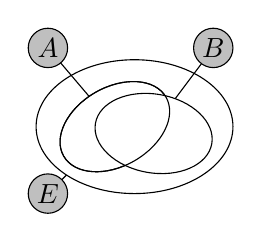
\begin{tikzpicture}[scale=.5]
                      \draw (-1.7,-1.7) -- (0,0);
                      \draw [fill = gray!50](-1.7,-1.7) circle(.5) node{$E$};
                      \draw [fill = white](0.5,0) ellipse (2.5 and 1.7);

                      \draw (-1.7,2) -- (0,0);
                      \draw [fill = gray!50](-1.7,2) circle(.5) node{$A$};
                      \draw [rotate=30,fill = white](0,0) ellipse (1.5 and 1);

                      \draw (2.5,2) -- (1,0);
                      \draw [fill = gray!50](2.5,2) circle(.5) node{$B$};
                      \draw [rotate=-10, fill = white](1,0) ellipse (1.5 and 1);

                      \draw [rotate=30](0,0) ellipse (1.5 and 1);
                  \end{tikzpicture}
            \item 	$\overline{A\cap B}$\\

                  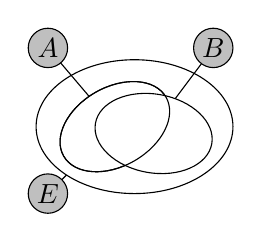
\begin{tikzpicture}[scale=.5]
                      \draw (-1.7,-1.7) -- (0,0);
                      \draw [fill = gray!50](-1.7,-1.7) circle(.5) node{$E$};
                      \draw [fill = white](0.5,0) ellipse (2.5 and 1.7);

                      \draw (-1.7,2) -- (0,0);
                      \draw [fill = gray!50](-1.7,2) circle(.5) node{$A$};
                      \draw [rotate=30,fill = white](0,0) ellipse (1.5 and 1);

                      \draw (2.5,2) -- (1,0);
                      \draw [fill = gray!50](2.5,2) circle(.5) node{$B$};
                      \draw [rotate=-10, fill = white](1,0) ellipse (1.5 and 1);

                      \draw [rotate=30](0,0) ellipse (1.5 and 1);
                  \end{tikzpicture}
            \item 	$\overline{A\cup B}$\\

                  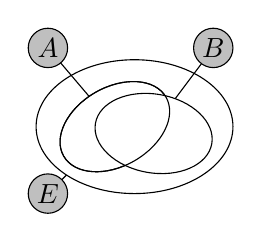
\begin{tikzpicture}[scale=.5]
                      \draw (-1.7,-1.7) -- (0,0);
                      \draw [fill = gray!50](-1.7,-1.7) circle(.5) node{$E$};
                      \draw [fill = white](0.5,0) ellipse (2.5 and 1.7);

                      \draw (-1.7,2) -- (0,0);
                      \draw [fill = gray!50](-1.7,2) circle(.5) node{$A$};
                      \draw [rotate=30,fill = white](0,0) ellipse (1.5 and 1);

                      \draw (2.5,2) -- (1,0);
                      \draw [fill = gray!50](2.5,2) circle(.5) node{$B$};
                      \draw [rotate=-10, fill = white](1,0) ellipse (1.5 and 1);

                      \draw [rotate=30](0,0) ellipse (1.5 and 1);
                  \end{tikzpicture}

            \item 	$\overline{A}\cap \overline{B}$\\

                  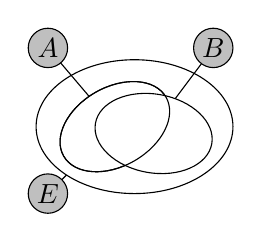
\begin{tikzpicture}[scale=.5]
                      \draw (-1.7,-1.7) -- (0,0);
                      \draw [fill = gray!50](-1.7,-1.7) circle(.5) node{$E$};
                      \draw [fill = white](0.5,0) ellipse (2.5 and 1.7);

                      \draw (-1.7,2) -- (0,0);
                      \draw [fill = gray!50](-1.7,2) circle(.5) node{$A$};
                      \draw [rotate=30,fill = white](0,0) ellipse (1.5 and 1);

                      \draw (2.5,2) -- (1,0);
                      \draw [fill = gray!50](2.5,2) circle(.5) node{$B$};
                      \draw [rotate=-10, fill = white](1,0) ellipse (1.5 and 1);

                      \draw [rotate=30](0,0) ellipse (1.5 and 1);
                  \end{tikzpicture}

            \item 	$\overline{A}\cup\overline{B}$\\

                  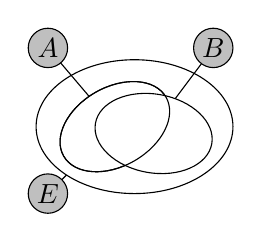
\begin{tikzpicture}[scale=.5]
                      \draw (-1.7,-1.7) -- (0,0);
                      \draw [fill = gray!50](-1.7,-1.7) circle(.5) node{$E$};
                      \draw [fill = white](0.5,0) ellipse (2.5 and 1.7);

                      \draw (-1.7,2) -- (0,0);
                      \draw [fill = gray!50](-1.7,2) circle(.5) node{$A$};
                      \draw [rotate=30,fill = white](0,0) ellipse (1.5 and 1);

                      \draw (2.5,2) -- (1,0);
                      \draw [fill = gray!50](2.5,2) circle(.5) node{$B$};
                      \draw [rotate=-10, fill = white](1,0) ellipse (1.5 and 1);

                      \draw [rotate=30](0,0) ellipse (1.5 and 1);
                  \end{tikzpicture}



            \item 	$\overline{A\cap \overline{B}}$\\

                  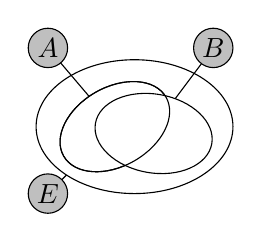
\begin{tikzpicture}[scale=.5]
                      \draw (-1.7,-1.7) -- (0,0);
                      \draw [fill = gray!50](-1.7,-1.7) circle(.5) node{$E$};
                      \draw [fill = white](0.5,0) ellipse (2.5 and 1.7);

                      \draw (-1.7,2) -- (0,0);
                      \draw [fill = gray!50](-1.7,2) circle(.5) node{$A$};
                      \draw [rotate=30,fill = white](0,0) ellipse (1.5 and 1);

                      \draw (2.5,2) -- (1,0);
                      \draw [fill = gray!50](2.5,2) circle(.5) node{$B$};
                      \draw [rotate=-10, fill = white](1,0) ellipse (1.5 and 1);

                      \draw [rotate=30](0,0) ellipse (1.5 and 1);
                  \end{tikzpicture}

            \item 	$(A\cap\overline{B})\cup(A\cap B)$\\

                  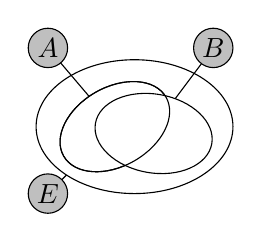
\begin{tikzpicture}[scale=.5]
                      \draw (-1.7,-1.7) -- (0,0);
                      \draw [fill = gray!50](-1.7,-1.7) circle(.5) node{$E$};
                      \draw [fill = white](0.5,0) ellipse (2.5 and 1.7);

                      \draw (-1.7,2) -- (0,0);
                      \draw [fill = gray!50](-1.7,2) circle(.5) node{$A$};
                      \draw [rotate=30,fill = white](0,0) ellipse (1.5 and 1);

                      \draw (2.5,2) -- (1,0);
                      \draw [fill = gray!50](2.5,2) circle(.5) node{$B$};
                      \draw [rotate=-10, fill = white](1,0) ellipse (1.5 and 1);

                      \draw [rotate=30](0,0) ellipse (1.5 and 1);
                  \end{tikzpicture}

            \item 	$(A\cap\overline{B})\cup(\overline{A}\cap{B})$\\

                  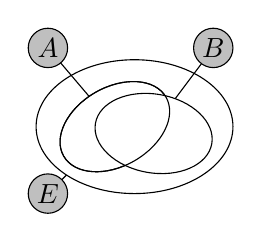
\begin{tikzpicture}[scale=.5]
                      \draw (-1.7,-1.7) -- (0,0);
                      \draw [fill = gray!50](-1.7,-1.7) circle(.5) node{$E$};
                      \draw [fill = white](0.5,0) ellipse (2.5 and 1.7);

                      \draw (-1.7,2) -- (0,0);
                      \draw [fill = gray!50](-1.7,2) circle(.5) node{$A$};
                      \draw [rotate=30,fill = white](0,0) ellipse (1.5 and 1);

                      \draw (2.5,2) -- (1,0);
                      \draw [fill = gray!50](2.5,2) circle(.5) node{$B$};
                      \draw [rotate=-10, fill = white](1,0) ellipse (1.5 and 1);

                      \draw [rotate=30](0,0) ellipse (1.5 and 1);
                  \end{tikzpicture}
        \end{enumerate}
    \end{multicols}
\end{exercice}
\begin{remarque}[]
    Quand on considère 2 parties d'un ensemble E, leur union en est encore une, de même que leur intersection. Il en va encore de même pour le complémentaire d'une partie de E. Ces trois opérations sont donc « internes »  à $\mathcal{P}(E)$, et on peut même énoncer le résultat suivant :
\end{remarque}

\begin{propriete}[]
    Soit $E$ un ensemble. Alors lorsqu'on munit $\mathcal{P}(E)$ de $\cup$, $\cap$ et de l'opération « complémentaire » , on obtient une \textit{algèbre de Boole} :\begin{itemize}
        \item 	0 se note $\emptyset$;
        \item 	1 se note $E$;
        \item 	+ se note $\cup$;
        \item 	$\times$ se note $\cap$.
    \end{itemize}
\end{propriete}
Cela implique qu'on peut effectuer les calculs dans $\mathcal{P}(E)$ de la même manière qu'on effectue les calculs booléens.
\begin{exemple}[]
    \begin{tabbing}
        $A\cup(B\cap \barmaj{A})$ \= $=(A\cup B)\cap(A\cup \barmaj{A})\qquad$ \=car $\cup$ se distribue sur $\cap$\\
        \> $= (A\cup B)\cap E$ \>puisque $A\cup \barmaj{A}=E$ (tout comme $a+\barmin{a}=1$)\\
        \> $= A\cup B$ \> car $E$ est neutre pour $\cap$ \\
        \> \>(tout comme $1$ est neutre pour $\times$)
    \end{tabbing}
\end{exemple}

On peut aussi utiliser des \textit{diagrammes de Venn} (les dessins « à base de patatoïdes »  vus plus haut) dans les cas simples.

\begin{exercice}[]
    Illustrer à l'aide d'un diagramme  que l'égalité $A\cap B = A\cap C$ n'entraîne pas automatiquement $B=C$.
\end{exercice}

\begin{propriete}[ : lois de De Morgan]
    Pour toutes parties $A$ et $B$ de $E$ on a
    $$\barmaj{A\cup B}=\barmaj{A}\cap\barmaj{B}\qquad\text{et}\qquad\barmaj{A\cap B}=\barmaj{A}\cup\barmaj{B}$$
    puisque  $\mathcal{P}(E)$  est une algèbre de Boole.
\end{propriete}
\begin{methode}[]
    Soient $A$ et $B$ deux parties de E, comment écrire l'ensemble $$F=\lbrace \,x\in E,\,x\in A\:et\:x\notin B\cup C\rbrace$$
    à l'aide d'union, intersection et complémentaire ?\\

    \begin{itemize}
        \item 	les « et »  représentent des $\cap$;
        \item 	les « ou »  représentent de $\cup$;
        \item 	pour tout ensemble $G$, $x\notin G$ équivaut à $x\in\barmaj{G}$.
    \end{itemize}

    Donc dans ce cas
    \begin{tabbing}
        $F$ \= $=A\cap\overline{B\cup C}\qquad$ et on utilise une loi de De Morgan\\
        \> $=A\cap \barmaj{B}\cap \barmaj{C}$
    \end{tabbing}
\end{methode}

\begin{exercice}[]
    Dans $\mathcal{P}(E)$ on définit l'opération $\Delta$ comme ceci :
    $$A\,\Delta\,B=\lbrace x\in E,\, x\in A\cup B\:et\:x\notin{A\cap B}\rbrace$$
    \begin{enumerate}
        \item 	Faire un diagramme de Venn et colorier $A\,\Delta\,B$.
        \item 	À quelle opération logique $\Delta$ correspond-elle ?
        \item 	Exprimer $\Delta$ à l'aide de $\cup$, $\cap$ et le complémentaire.
        \item 	Montrer par le calcul que $(A\,\Delta\,B)\,\Delta\,C =A\,\Delta\,(B\,\Delta\,C)$.
    \end{enumerate}
\end{exercice}

\begin{exercice}[]
    Dans $\mathcal{P}(E)$ on définit l'opération $\backslash$ comme ceci :
    $$A\backslash B=\lbrace x\in E,\, x\in A\:et\:x\notin B\rbrace$$
    \begin{enumerate}
        \item 	Faire un diagramme de Venn et colorier $A\backslash B$.
        \item 	Exprimer $\backslash$ à l'aide de $\cup$, $\cap$ et le complémentaire.
        \item 	Montrer par le calcul que $A\backslash (B\cap C)=(A\backslash B)\cup(A\backslash C)$.
    \end{enumerate}
\end{exercice}




\section{Produit cartésien}

\begin{definition}[ : produit cartésien de deux ensembles]
    Soient $E$ et $F$ deux ensembles, on appelle \textit{produit cartésien} de $E$ par $F$ et on note $E\times F$ l'ensemble des couples $(x;\,y)$, où $x\in E$ et $y\in F$.
    $$E\times F = \left\lbrace  (x;\,y),\:x\in E,\,y\in F\right\rbrace$$
\end{definition}

\begin{exemple}[s]
    \begin{itemize}
        \item 	Prenons $E=\left\lbrace bille;\,ballon\right\rbrace$ et $F=\left\lbrace rouge;\,vert;\,bleu\right\rbrace$ alors on peut représenter $E\times F$ de la manière suivante :

              \begin{center}
                  \tabstyle[UGLiBlue]
                  \begin{tabular}{|c|c|c|}
                      \hline\rowcolor{UGLiBlue}
                      \cellcolor{white}              & \ccell bille     & \ccell ballon     \\
                      \hline
                      \cellcolor{UGLiBlue}\ccell rouge & (bille; rouge) & (ballon; rouge) \\
                      \hline
                      \cellcolor{UGLiBlue}\ccell vert  & (bille; vert)  & (ballon; vert)  \\
                      \hline
                      \cellcolor{UGLiBlue}\ccell bleu  & (bille; bleu)  & (ballon; bleu)  \\
                      \hline
                  \end{tabular}
              \end{center}

        \item 	$\R\times\R$ se note aussi $\R^2$. Quand on s'est donné un repère du plan $\repaff$, alors tout point du plan possède un unique couple de coordonnées dans $\R^2$ et réciproquement, à tout couple de $\R^2$ correspond un unique point du plan. C'est pourquoi on identifie $\R^2$ au plan... et $R^3$ à l'espace.
        \item 	Le produit cartésien est fondamental dans le domaine des bases de données.
    \end{itemize}\end{exemple}

\begin{exercice}[]
    En prenant $E=\lbrace 1;\,2\rbrace$ et $F=\lbrace a;\,b;\,c\rbrace$ construire $E\times F$ et $F\times E$ et montrer que ces ensembles sont différents.
\end{exercice}

\begin{propriete}[]
    Si $\card(E)=n$ et $\card(F)=p$ alors $\card(E\times F)=n\times p$.
\end{propriete}

\begin{definition}[: produit cartésien de plusieurs ensembles]
    Soient $E_1$, \ldots $E_n$ $k$ ensembles ($n$ entier supérieur à 2), on note
    $$\prod_{k=1}^{k=n}E_k=E_1\times\ldots\times E_n$$
    l'ensemble des \textit{n-uplets} $(x_1;\,\ldots;\,x_n)$ ou chaque $x_k$ appartient à $E_k$.\\ On dit que c'est le \textit{produit cartésien} des ensembles $E_k$.
\end{definition}

\begin{propriete}[]
    Quand tous les ensembles sont finis, le cardinal de l'ensemble produit s'obtient en multipliant les cardinaux des ensembles.
\end{propriete}
\section{Relations binaires}
\begin{definition}[ : relation binaire]
    Soient $E$ et $F$ deux ensembles. Une \textit{relation binaire de $E$ vers $F$} c'est la donnée de certains \textit{couples} $(x_i;\,y_i)$; où $x_i\in E$ et $y_i\in F$.\\
    $E$ est appelé \textit{ensemble de départ} et $F$ \textit{ensemble d'arrivée}.
    L'ensemble de ces couples (notons-le $G$), est appelé le \textit{graphe} de la relation. C'est une partie de $E\times F$.
\end{definition}

\begin{exemple}[ : avec un diagramme sagittal]
    \begin{center}
        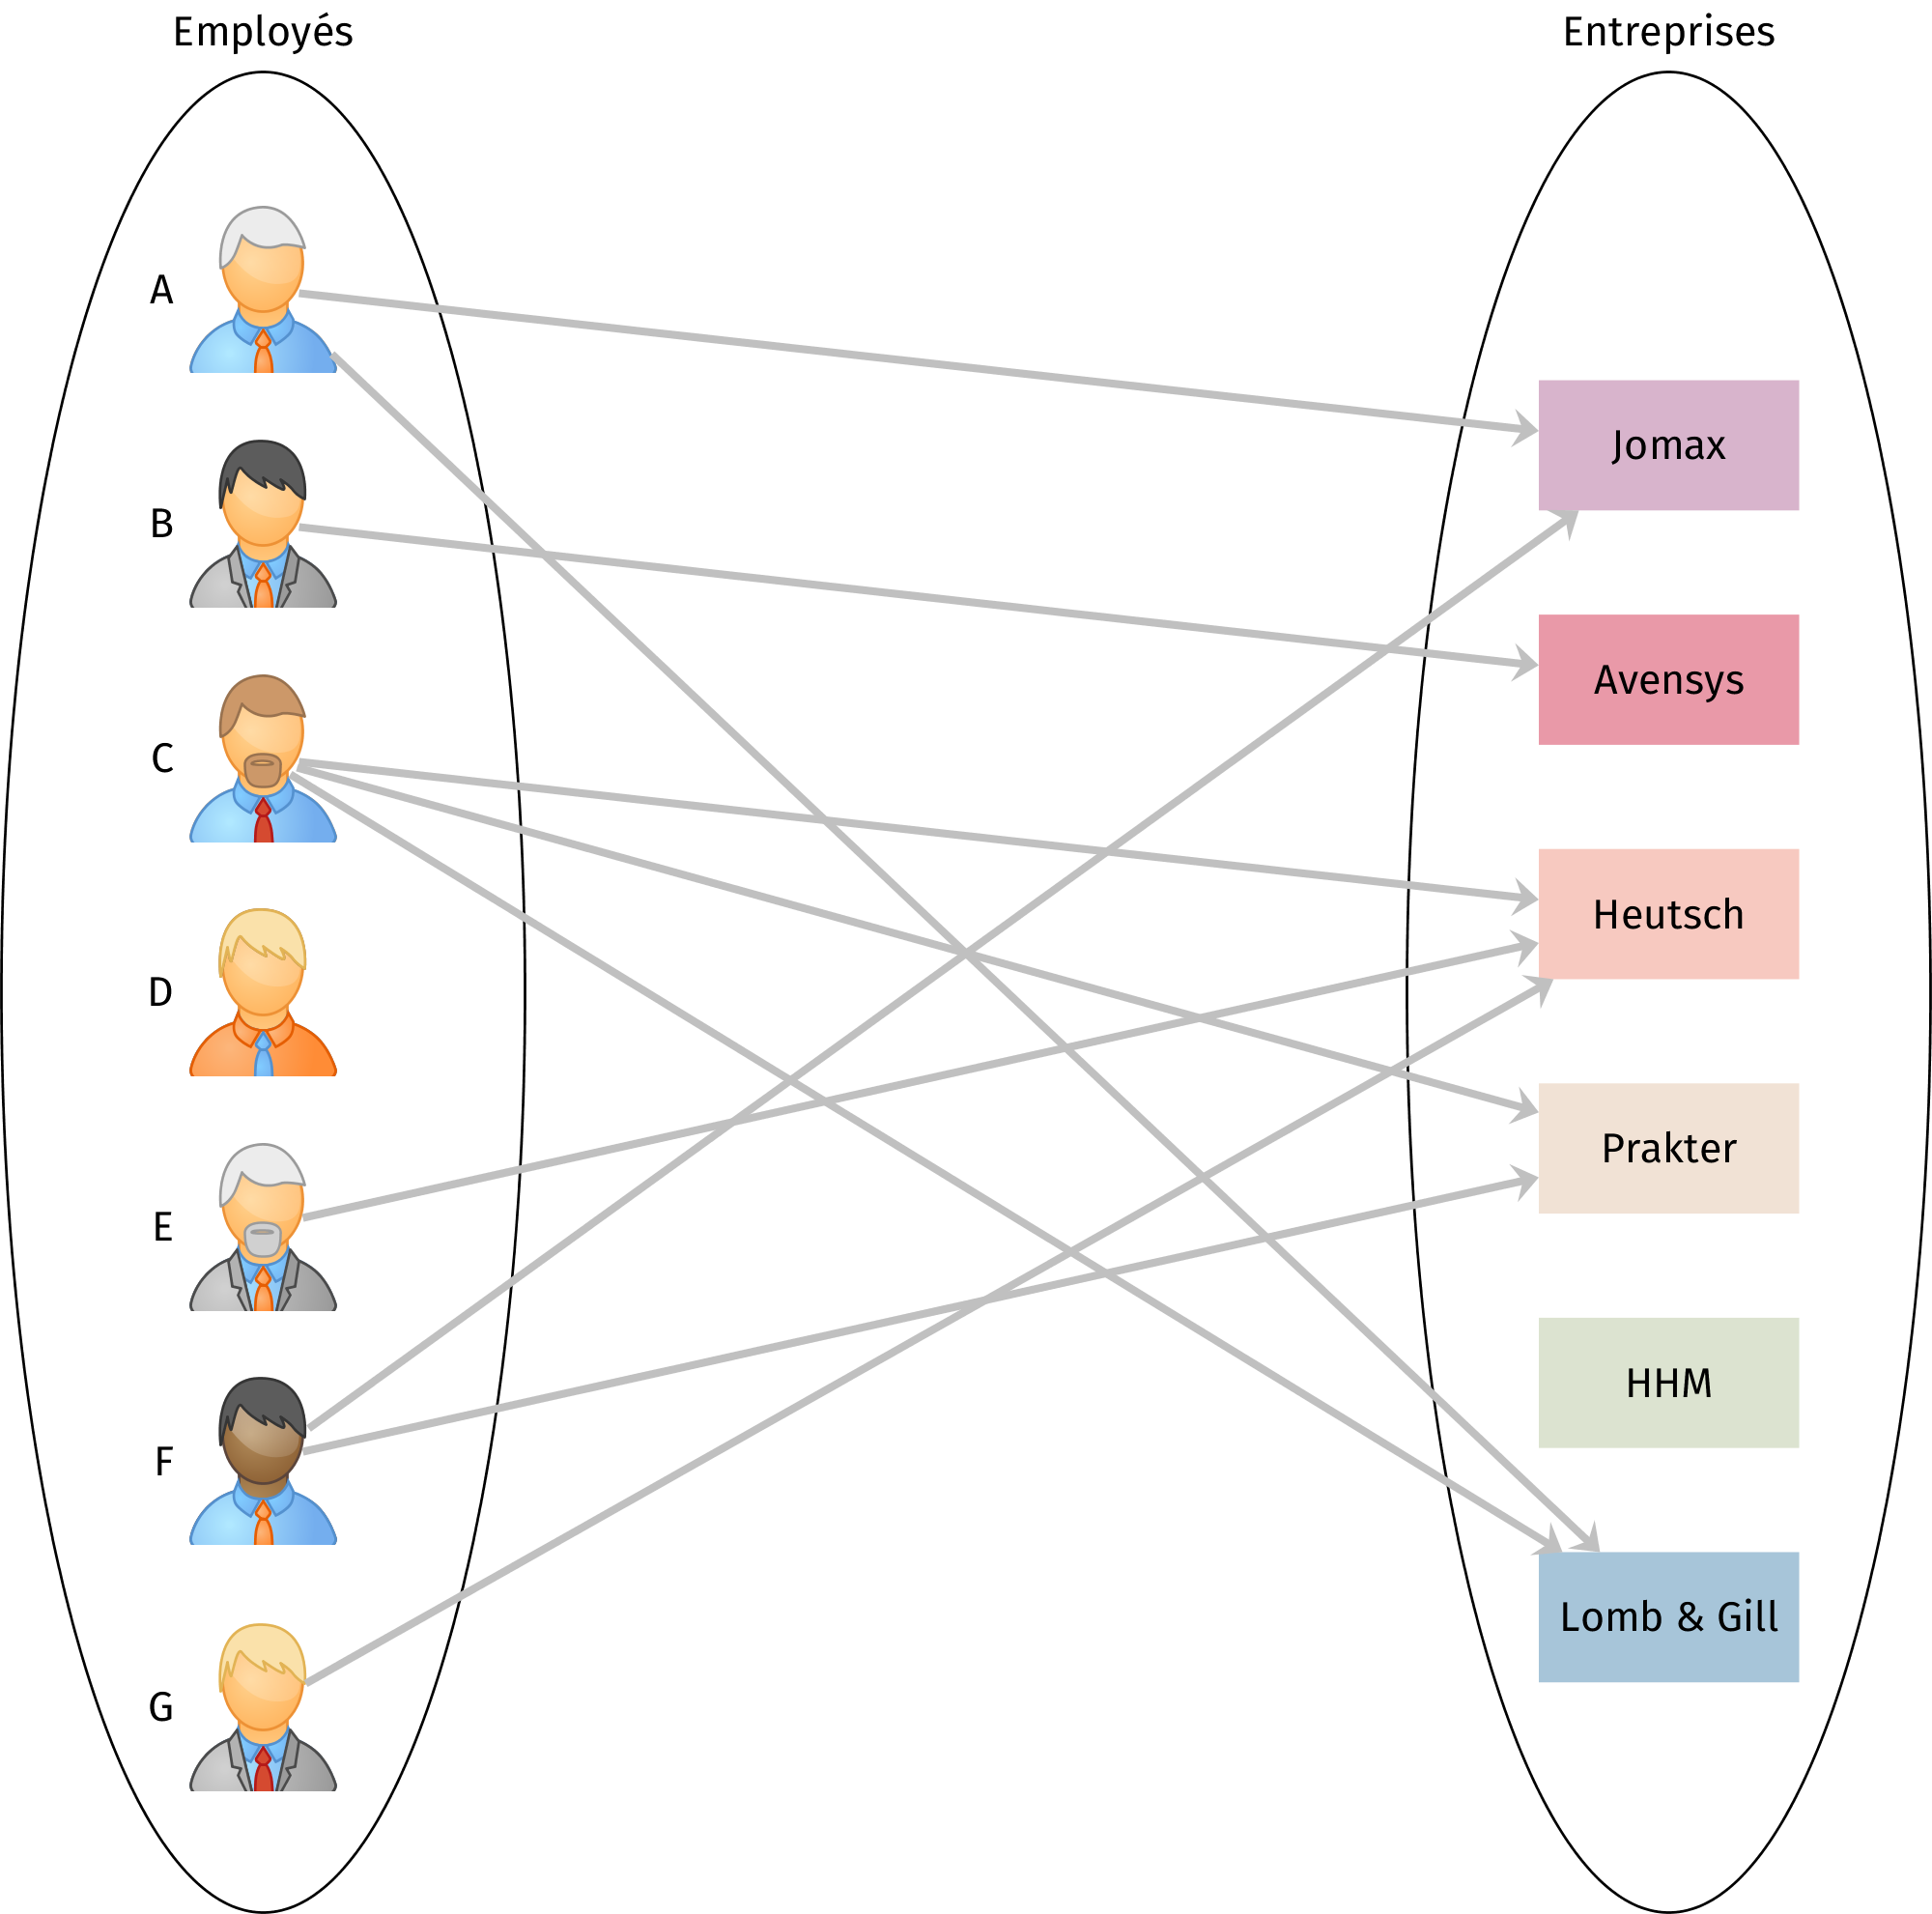
\includegraphics[width=9cm]{ensembles/img/graphe_relation_binaire.png}
    \end{center}
    On considère un ensemble $E$ d'employés, un ensemble $F$ d'entreprises et la relation « ... est ou a été un employé de ... » .
    \begin{itemize}
        \item 	$(A;\,Jomax)\in G$ : l'employé $A$ a travaillé pour l'entreprise Jomax;
        \item 	on a aussi $(A;\,Lomb\,\&\,Gill)\in G$ car cet employé a aussi occupé un poste là-bas;
        \item 	$D$ n'a pas occupé de postes dans $F$.
        \item 	HHM n'a aucun employé de $E$.
    \end{itemize}
    $G$ est ici représenté par l'ensemble des flèches.
\end{exemple}

\begin{exemple}[ : avec un tableau]

    Voici la même relation :\\
    \begin{center}
        \tabstyled
        \begin{tabular}{|l|>{\centering\arraybackslash}m{.7cm}|>{\centering\arraybackslash}m{.7cm}|>{\centering\arraybackslash}m{.7cm}|>{\centering\arraybackslash}m{.7cm}|>{\centering\arraybackslash}m{.7cm}|>{\centering\arraybackslash}m{.7cm}|>{\centering\arraybackslash}m{.7cm}|}
            \hline
            \cellcolor{white}                     & \cellcolor{UGLiBlue}\ccell A & \cellcolor{UGLiBlue}\ccell B & \cellcolor{UGLiBlue}\ccell C & \cellcolor{UGLiBlue}\ccell D & \cellcolor{UGLiBlue}\ccell E & \cellcolor{UGLiBlue}\ccell F & \cellcolor{UGLiBlue}\ccell G \\
            \hline
            \cellcolor{UGLiBlue}\ccell Jomax        & x                          &                            &                            &                            &                            & x                          &                            \\
            \hline
            \cellcolor{UGLiBlue}\ccell Avensys      &                            & x                          &                            &                            &                            &                            &                            \\
            \hline
            \cellcolor{UGLiBlue}\ccell Heutsch      &                            &                            & x                          &                            & x                          &                            & x                          \\
            \hline
            \cellcolor{UGLiBlue}\ccell Prakter      &                            &                            & x                          &                            &                            & x                          &                            \\
            \hline
            \cellcolor{UGLiBlue}\ccell HHM          &                            &                            &                            &                            &                            &                            &                            \\
            \hline
            \cellcolor{UGLiBlue}\ccell Lomb \& Gill & x                          &                            & x                          &                            &                            &                            &                            \\
            \hline
        \end{tabular}
    \end{center}
\end{exemple}

Nous étudierons plus en détail les relations binaires pour lesquelles l'ensemble de départ et d'arrivée sont les mêmes.

\begin{definition}[ : relation binaire dans un ensemble]
    Quand $E=F$ on parle de \textit{relation binaire dans} $E$.
\end{definition}

\begin{exemple}[s]

    \begin{itemize}
        \item 	L'égalité de deux entiers naturels est une relation binaire dans $\N$.
        \item 	Posons $E=\N^*$ et disons que $x\mathcal{R}y$ si et seulement si $x$ divise $y$. On obtient une relation binaire.
        \item 	Dans l'ensemble $\mathcal{D}$ des droites du plan disons que $d\mathcal{R}d'$ si et seulement si $d\perp d'$. On obtient une relation binaire.
    \end{itemize}
\end{exemple}

\begin{definition}[s : réflexivité, symétrie, antisymétrie, transitivité]
    Soit $\mathcal{R}$ une relation binaire sur E, on dit que $\mathcal{R}$ est
    \begin{itemize}
        \item 	\textit{réflexive} si tout élément est en relation avec lui-même : $\forall x\in E,\, x\mathcal{R}x$;
        \item 	\textit{symétrique} si dès que $x\mathcal{R}y$, cela entraîne $y\mathcal{R}x$ (et vice versa, évidemment);
        \item 	\textit{antisymétrique} si deux éléments différents ne peuvent être en relation « dans les deux sens  » .\\
              Cela revient à dire que si on trouve $x\mathcal{R}y$ et $y\mathcal{R}x$, alors nécessairement $x=y$;
        \item 	\textit{transitive} si lorsque $x\mathcal{R}y$ et $y\mathcal{R}z$ alors on a $x\mathcal{R}z$.
    \end{itemize}
\end{definition}
\begin{exemple}[s]

    $\mathcal{R}$ est réflexive. Tout élément est en relation avec lui même :
    \begin{center}
        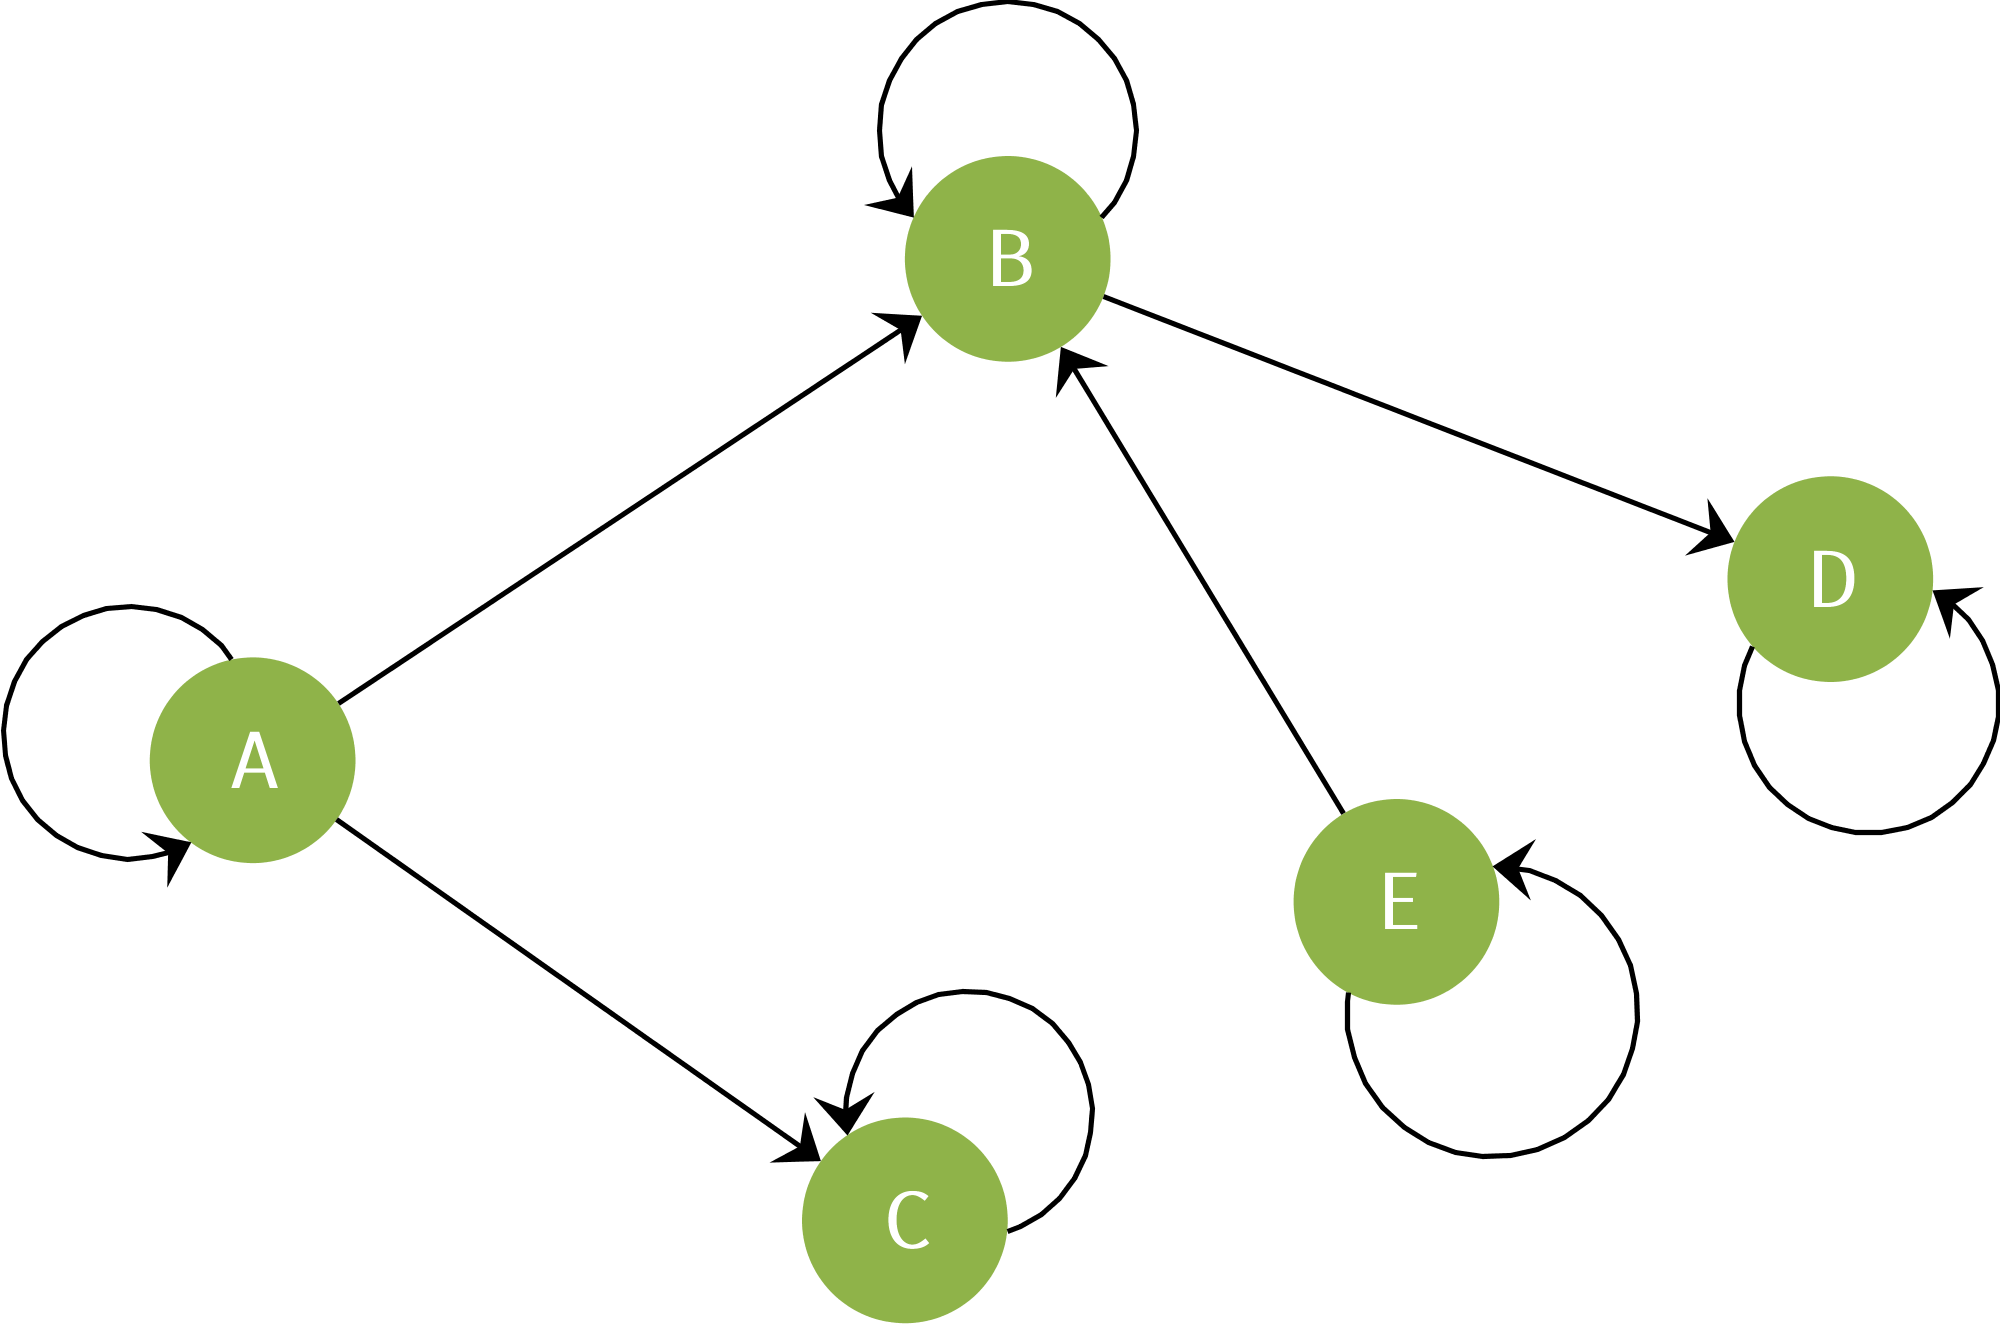
\includegraphics[width=7cm]{ensembles/img/relation_reflexive}
    \end{center}


    $\mathcal{R}$ est symétrique. Si $x\mathcal{R}y$ alors $y\mathcal{R}x$ de sorte que les éléments en relation le sont « dans les deux sens » :

    \begin{center}
        \includegraphics[width=7cm]{ensembles/img/relation_symétrique.png}
    \end{center}


    $\mathcal{R}$ est antisymétrique. Si une relation est vraie « dans les deux sens »  alors c'est qu'elle ne concerne qu'un élément : il n'y a pas de double flèche reliant deux éléments différents mais, peut-être, des cas comme $D\mathcal{R}D$ ou $E\mathcal{R}E$:
    \begin{center}
        \includegraphics[width=7cm]{ensembles/img/relation_antisymétrique.png}
    \end{center}


    $\mathcal{R}$ est transitive. À chaque fois qu'on peut « enchaîner »  les relations, le « raccourci »  est présent aussi :
    \begin{center}
        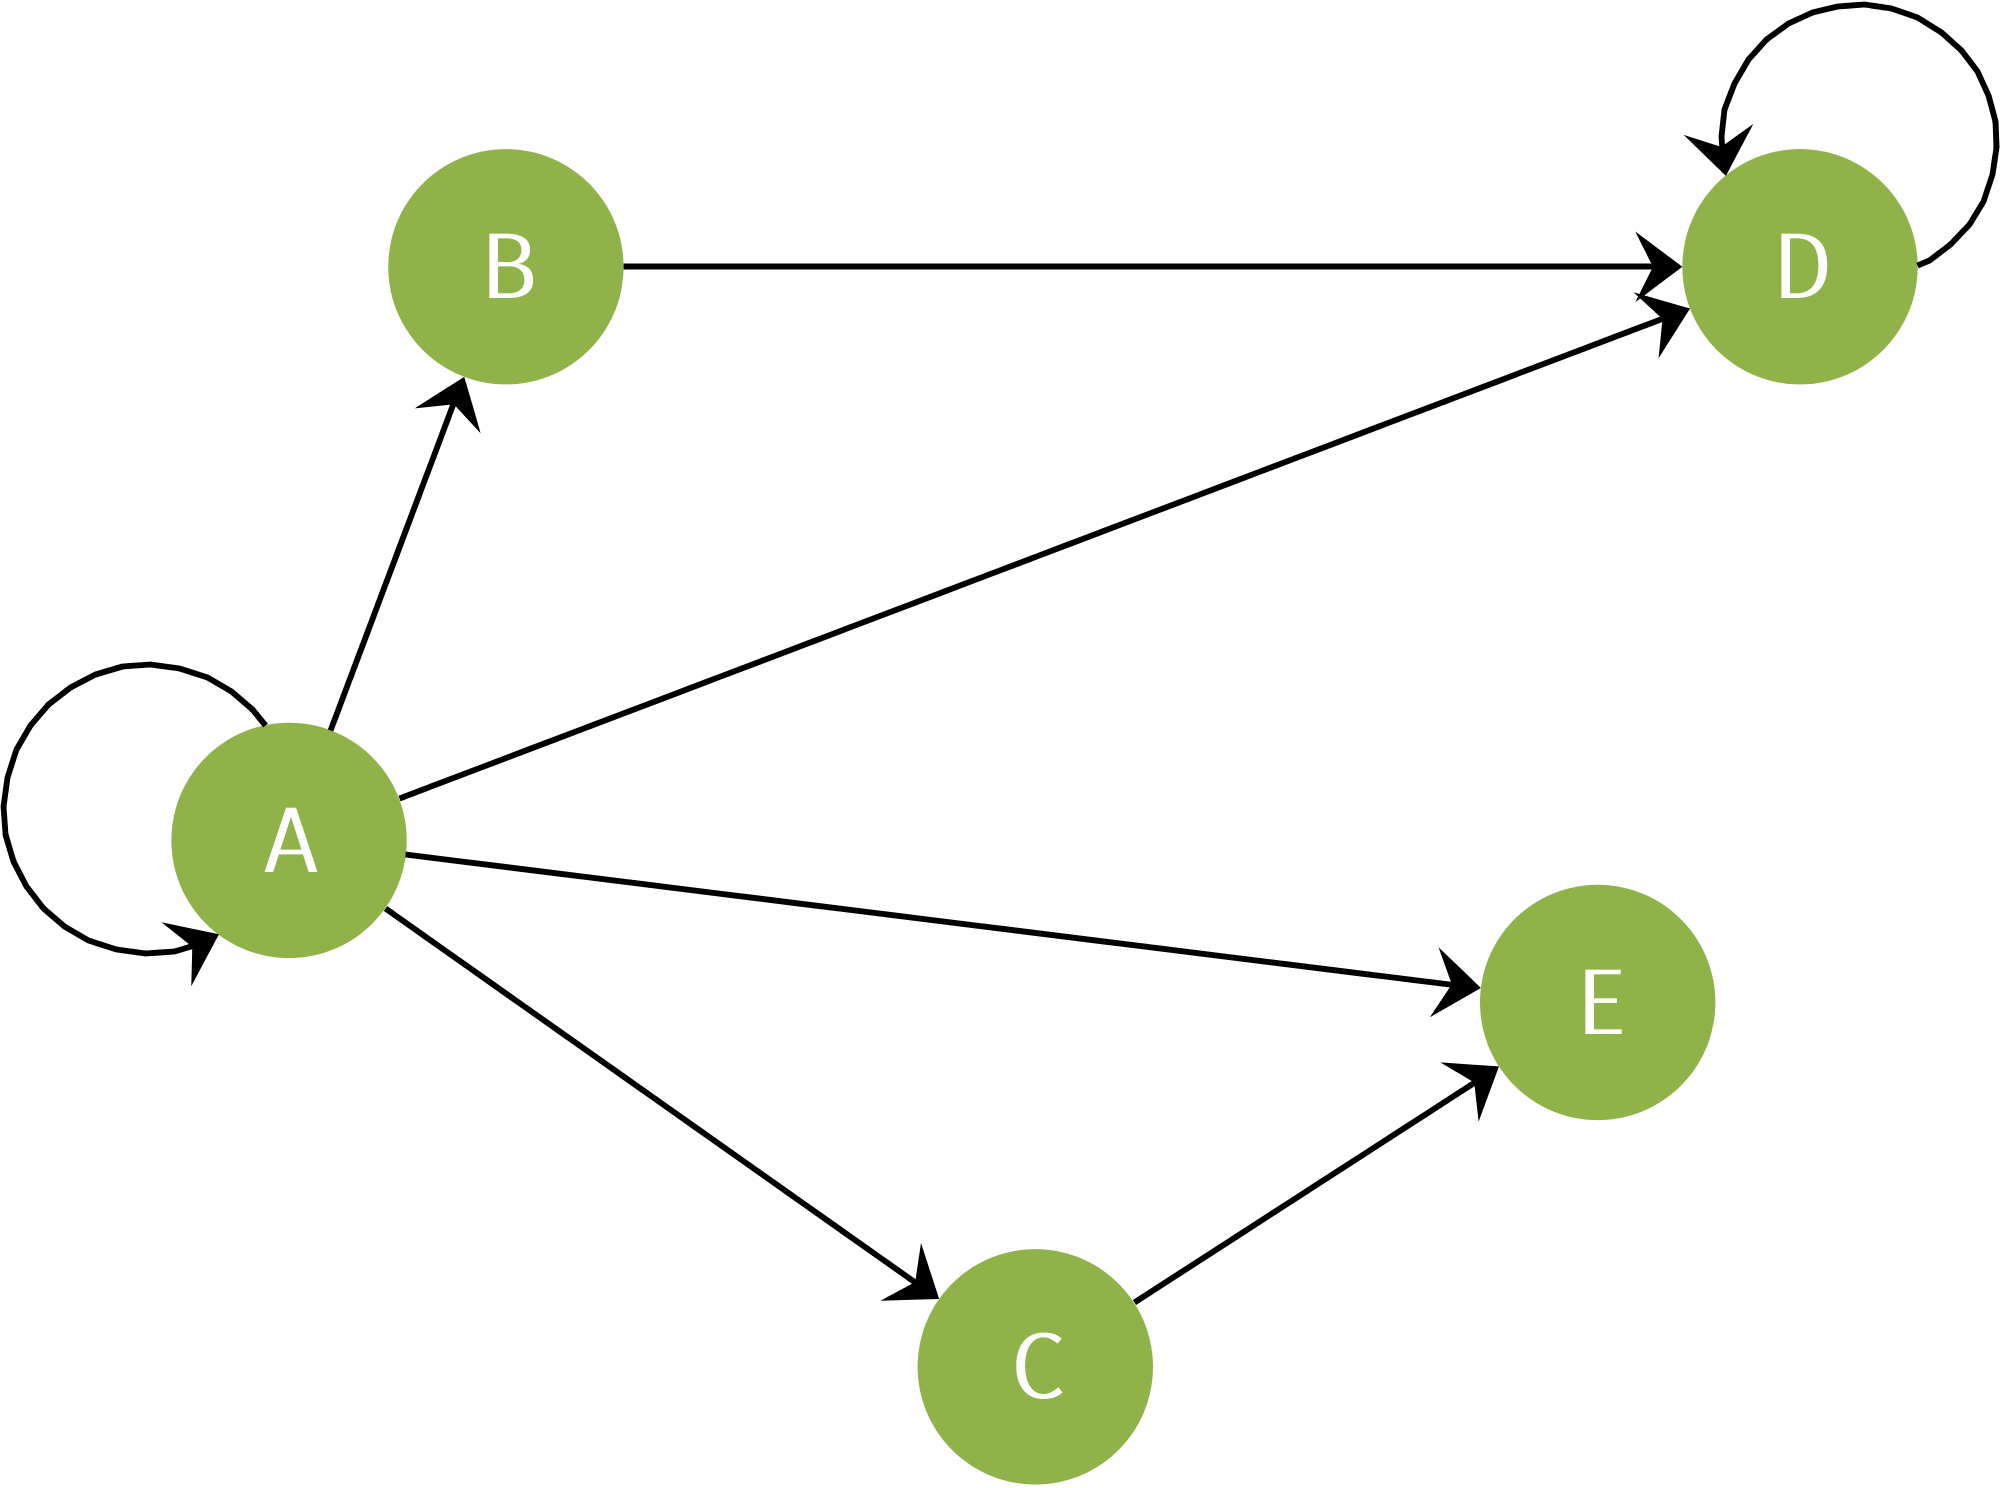
\includegraphics[width=7cm]{ensembles/img/relation_transitive.png}
    \end{center}
\end{exemple}

\begin{definition}[s : relation d'équivalence, relation d'ordre]
    \begin{itemize}
        \item 	Lorsqu'une relation binaire dans E est réflexive, symétrique et transitive, on dit que c'est une relation d'équivalence sur E.\\
              Une relation d'équivalence permet de partager E en \textit{classes} d'éléments qui sont tous équivalents (considérés « pareils »  pour la relation).
        \item 	Lorsqu'une relation binaire dans E est réflexive, antisymétrique et transitive, on dit que c'est une relation d'ordre sur E.\\
              Une relation d'ordre permet de « ranger les éléments comparables  »  :
              \begin{itemize}
                  \item 	Si à chaque fois qu'on prend deux éléments \textit{distincts} $x$ et $y$ alors on a $x\mathcal{R}y$ ou $y\mathcal{R}x$ alors l'ordre est dit \textit{total} car on peut toujours comparer deux éléments différents.
                  \item 	Si ce n'est pas le cas on parle d'ordre partiel.
              \end{itemize}
    \end{itemize}
\end{definition}

\begin{exemple}[s]
    \begin{itemize}
        \item 	Dans $N$, la relation d'égalité est une relation d'équivalence.
        \item 	Dans $\R$ la relation $\leqslant$ est une relation d'ordre totale.
        \item 	Dans l'ensemble des droites du plan, la relation de parallélisme est une relation d'équivalence.
        \item 	On considère $\R^2$ et on l'identifie à l'ensemble des points du plan muni d'un repère $\repaff$.
              On décide de noter $\preceq$ la relation suivante :\\ $(x_1,y_1)\preceq(x_2,y_2)$ si et seulement si $x_1\leqslant x_2$ et $y_1\leqslant y_2$.
              \begin{center}
                  \begin{tikzpicture}[]
                      \draw[fill=white](-1,-1) rectangle (7,7);
                      \repereal{-1}{-1}{7}{7}
                      \pointc{2}{6}{2}{4}{A}
                      \pointc{1}{2}{1}{2}{B}
                      \pointc{5}{3}{5}{3}{C}
                  \end{tikzpicture}
              \end{center}
    \end{itemize}
    alors $\preceq$ est une relation d'ordre, mais c'est ordre n'est pas total  : On a bien $\pc{}{1}{2}\preceq\pc{}{2}{4}$ mais on ne peut pas comparer $\pc{}{2}{4}$ et $\pc{}{5}{3}$.
\end{exemple}

\begin{encadrecolore}{Question}{UGLiOrange}
    Dans $\R$, la relation < est-elle une relation d'ordre ?
\end{encadrecolore}

\begin{exercice}[]
    La relation binaire $\mathcal{R}$ est elle réflexive, symétrique, antisymétrique, transitive ? Est-ce une relation d'équivalence ou d'ordre ? Si c'est une relation d'ordre est elle totale ou partielle ?
    \begin{itemize}
        \item 	Dans $\R$, $x\mathcal{R}y\,\Leftrightarrow\, x<y$.
        \item 	Dans $\N$, $x\mathcal{R}y\,\Leftrightarrow\,x$ divise y.
        \item 	Soit E un ensemble, dans $\mathcal{P}(E)$, $A\mathcal{R}B\,\Leftrightarrow\, A\subset B$.
        \item 	Soit E un ensemble, dans $\mathcal{P}(E)$, $A\mathcal{R}B\,\Leftrightarrow\, A\cap B=\emptyset$.\\
    \end{itemize}
\end{exercice}

\begin{exercice}[]
    \begin{center}
        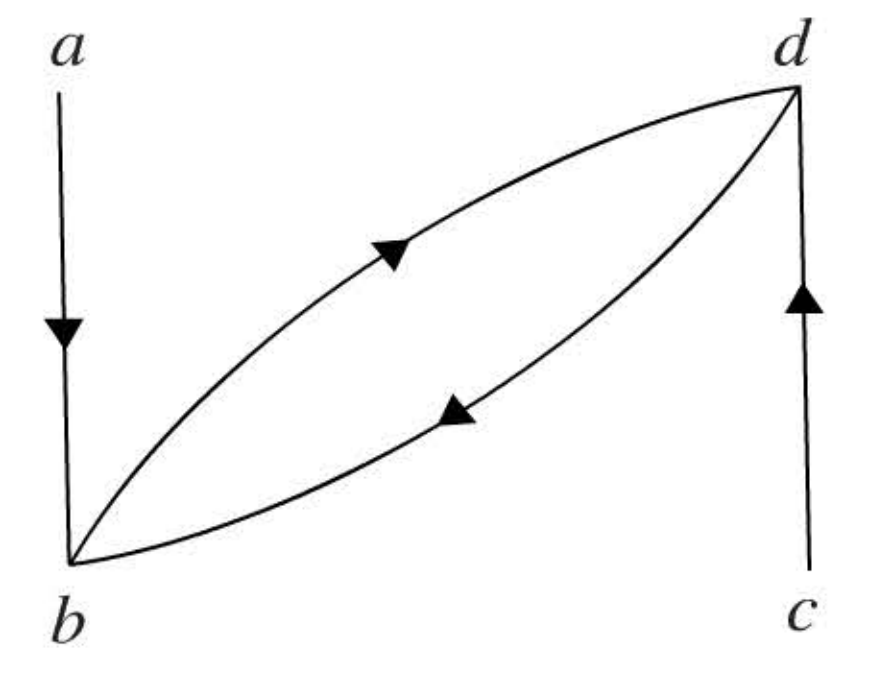
\includegraphics[width=5cm]{ensembles/img/graphe.PNG}
    \end{center}


    On considère le dessin comme étant la représentation d'une relation binaire, que l'on note $\mathcal{R}$ . définie sur l'ensemble $S = \lbrace  a;b;c;d\rbrace$ .

    \begin{enumalph}
        \item 	Écrire tous les éléments qui sont en relation sou s la forme $x\mathcal{R}y$, avec $(x;y) \in S^2$ .
        \item 	La relation R est elle réflexive ?
        \item 	La relation R est elle symétrique ?
        \item 	La relation R est elle transitive ?
        \item 	Au minimum, quelles flèches doit-on ajouter pour obtenir la représentation d'une
        relation réflexive ?
        \item Même question avec une relation symétrique.
    \end{enumalph}
\end{exercice}

\begin{exercice}[]
    On considère l'\textit{arbre binaire suivant} et sur l'ensemble des nombres présents dans l'arbre, on définit une relation binaire : $x\mathcal{R}y$ si et seulement si $x=y$ on bien on peut passer de x à y ou de y à x par un chemin qui descend toujours par la droite.
    \begin{center}
        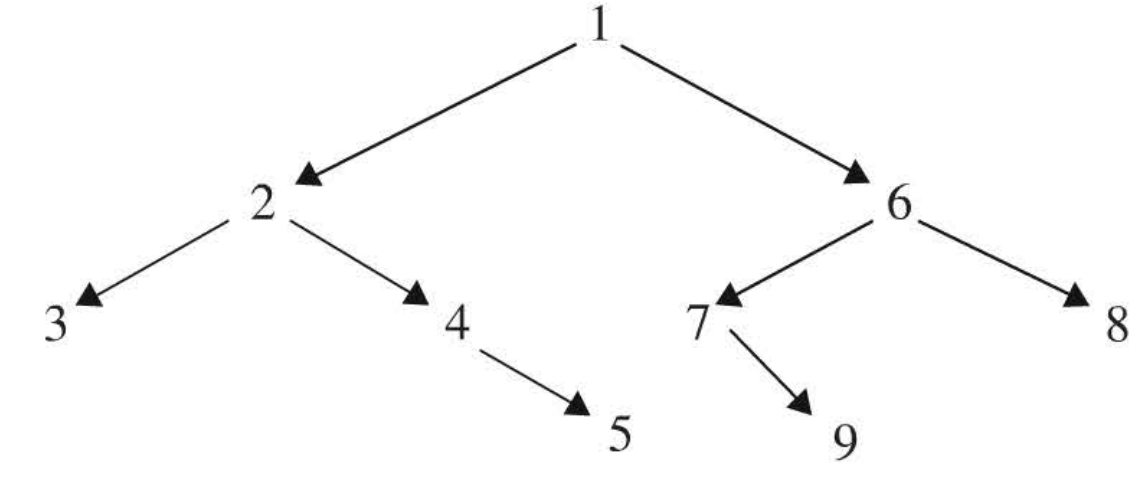
\includegraphics[width=8cm]{ensembles/img/arbre.PNG}
    \end{center}
    \begin{enumerate}
        \item 	Expliquer pourquoi simplement à partir de sa définition on peut affirmer que $\mathcal{R}$ est réflexive et symétrique.
        \item 	Montrer que $\mathcal{R}$ est une relation d'équivalence.
        \item 	Regrouper sur le schéma ci-dessus les nombres équivalents.
    \end{enumerate}
\end{exercice}

\begin{exercice}
    Dire si les relations suivantes sont réflexives, symétriques, antisymétriques, transitives.\\
    Dire ensuite si ce sont des relations d'équivalence, d'ordre total ou partiel.
    \begin{enumerate}
        \item 	Sur $\Z$, $x\mathcal{R}y\ \Longleftrightarrow\  x=-y$.
        \item 	Sur $\R^2$, $(x,\,y)\mathcal{R}(x'\,y')\ \Longleftrightarrow\ x=x'$.
        \item 	Soit $E$ un ensemble, sur $\mathcal{P}(E)$, $X\mathcal{R}Y\ \Longleftrightarrow\ X=Y\ \text{ou}\ X = \barmaj{Y}$.
        \item 	Sur $\Z$, $x\mathcal{R}y\ \Longleftrightarrow\  x+y$ est pair.
        \item 	Soit $E$ un ensemble et $A\subset E$, sur $\mathcal{P}(E)$, $X\mathcal{R}Y\ \Longleftrightarrow\ X\cup A=Y\cup A$.
    \end{enumerate}
\end{exercice}
\section{Applications}

\begin{definition}[s : application image, antécédents]
    Soient $E$ et $F$ deux ensembles. On appelle \textit{application} de $E$ dans $F$ une relation $\mathcal{R}$ binaire de $E$ vers $F$ telle que pour tout élément $x$ de $E$ \textit{il existe un unique} $y$ de $F$ tel que $x\mathcal{R}y$.\\

    L'usage est alors de noter $\mathcal{R}$ comme \textit{une fonction} :
    \begin{tabbing}
        $f\,:\,$ \=	$E\longrightarrow F$\\
        \>	$x \longmapsto y$\ \ où $y$ est l'unique élément de $F$ tel que $x\mathcal{R}y$.
    \end{tabbing}
    Et on écrit que $y=f(x)$.\\

    $y$ est appelé l'\textit{image} de $x$ par l'application $f$.\\
    On dit que $x$ est \textit{un antécédent} de $y$ par $f$.
\end{definition}

\begin{exemple}[s]
    Cette relation binaire n'est pas une application de l'ensemble Employés dans l'ensemble Entreprises car (par exemple), l'élément A est associé à 2 éléments de Entreprises
    \begin{center}
        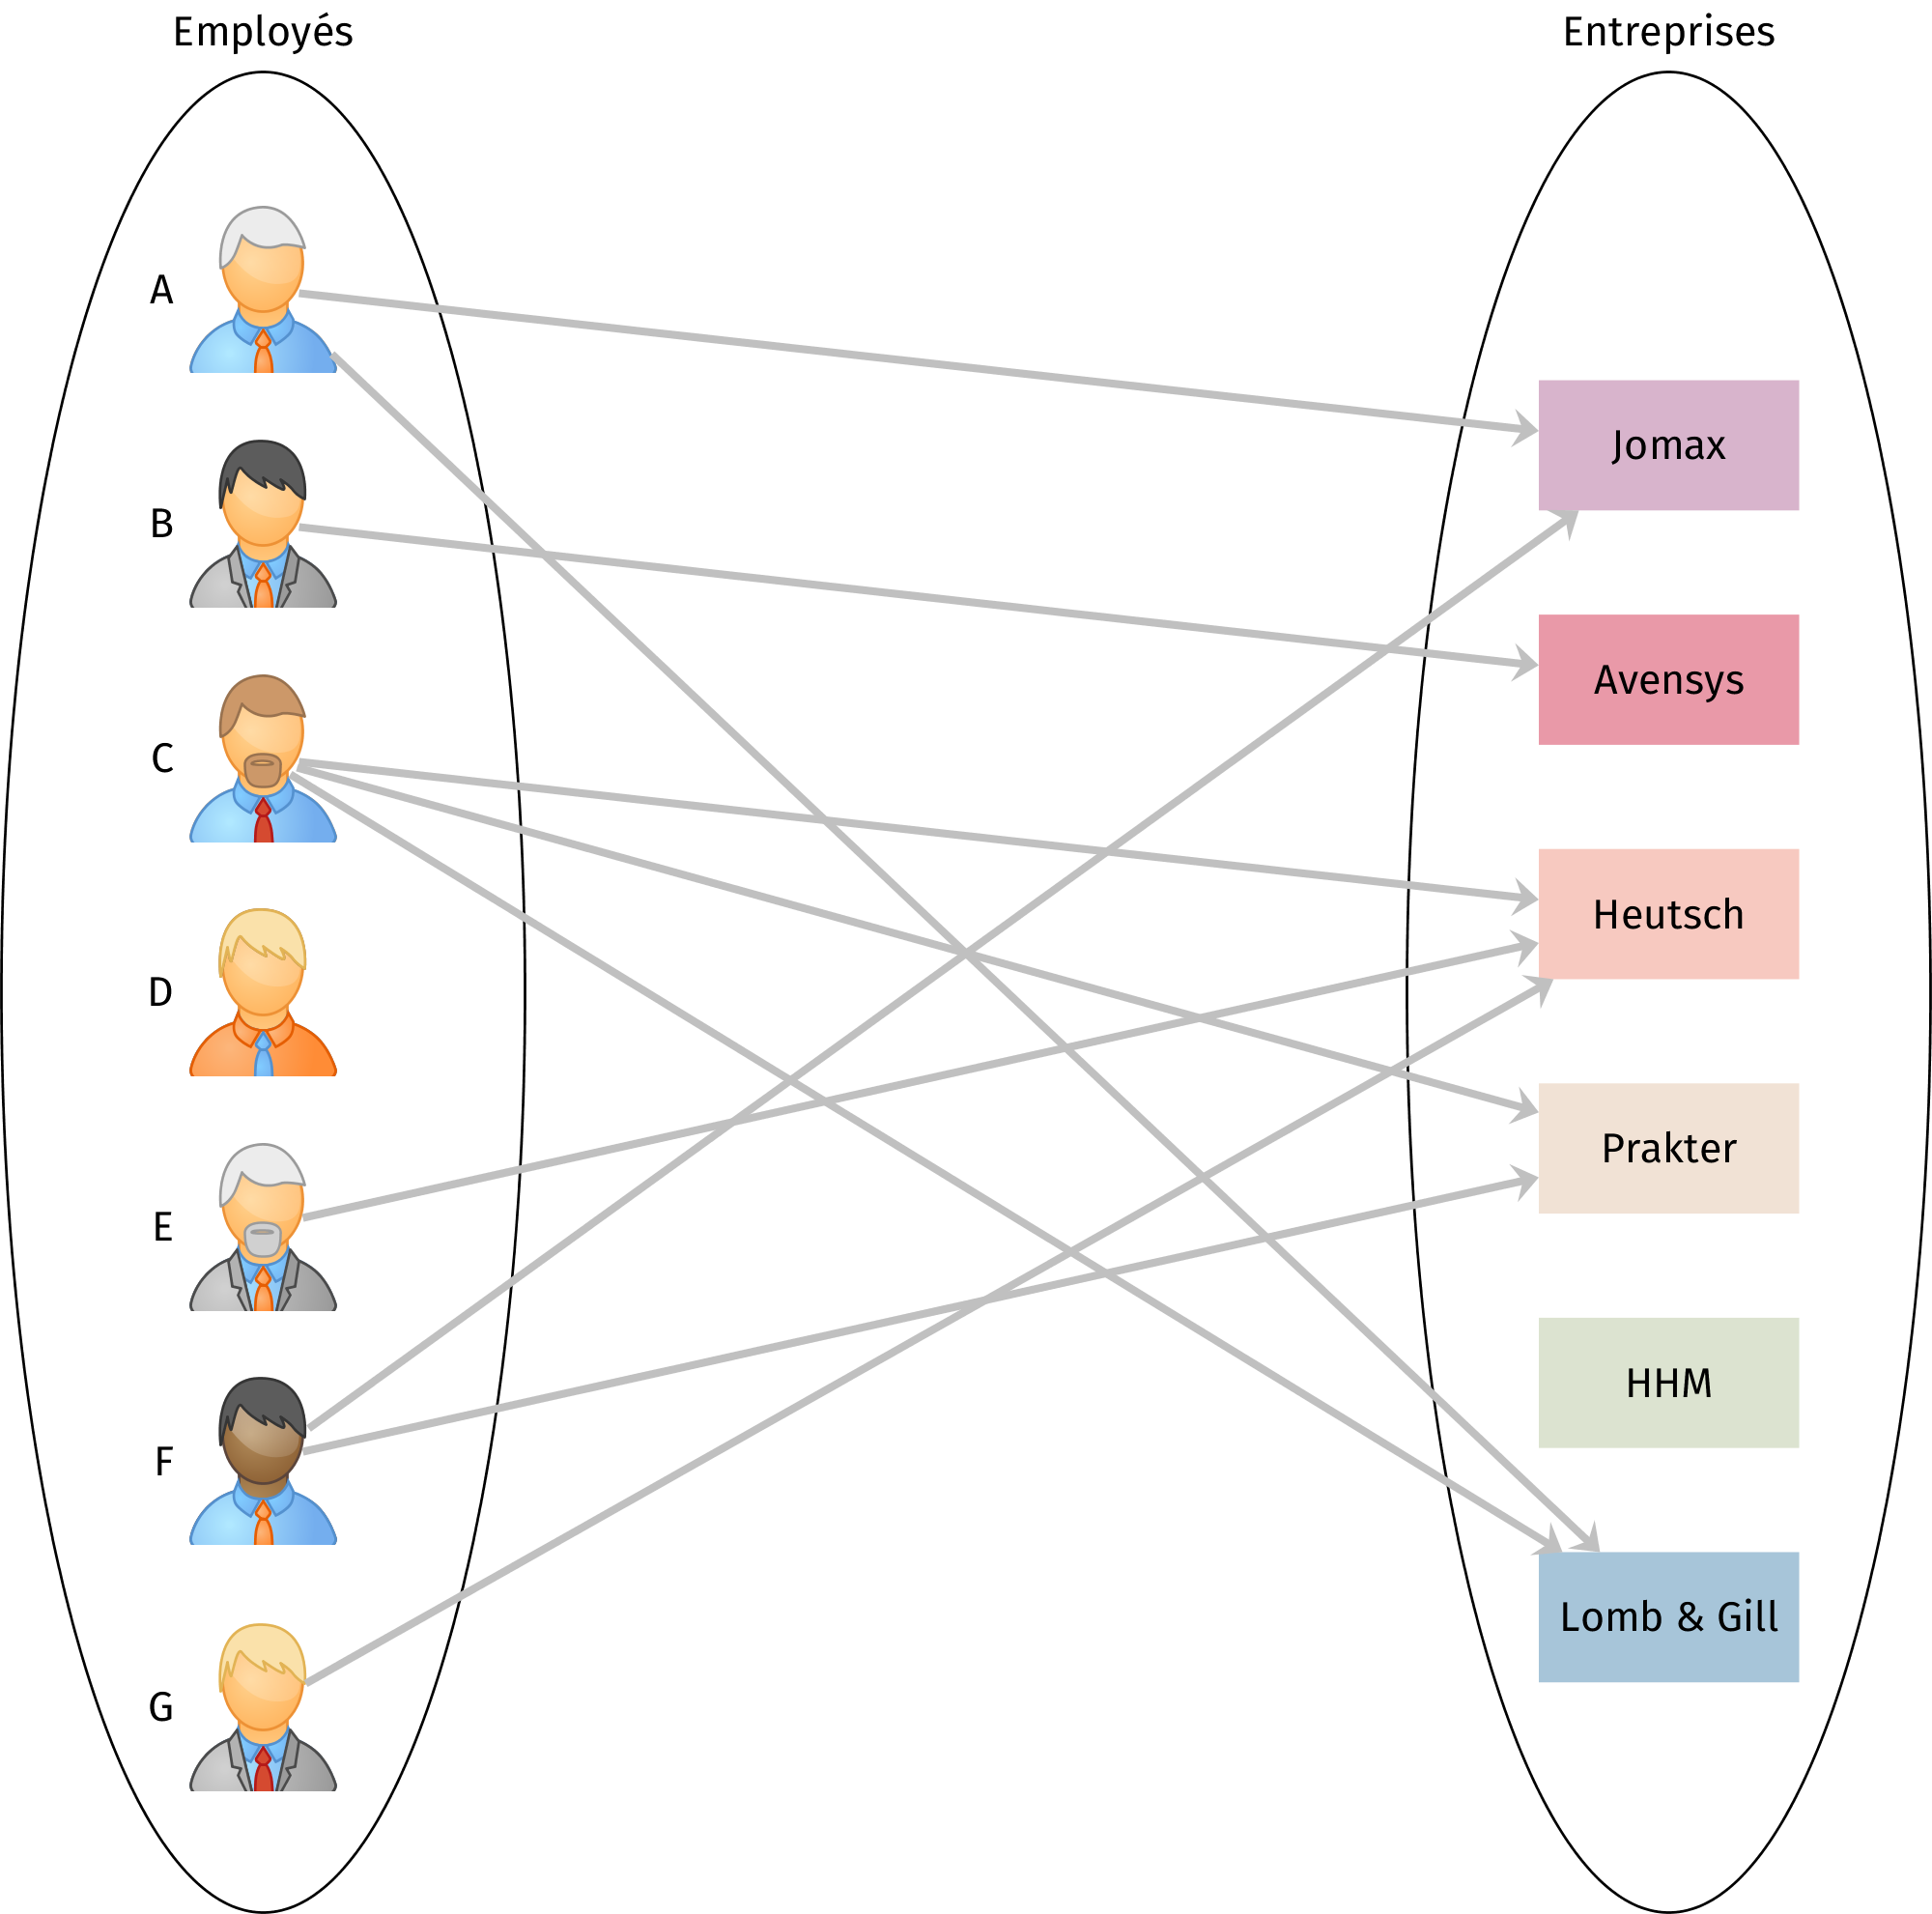
\includegraphics[width=7cm]{ensembles/img/graphe_relation_binaire.png}
    \end{center}
    Celle-ci n'en est pas une non plus car D n'est associé à aucun élément de Entreprises.
    \begin{center}
        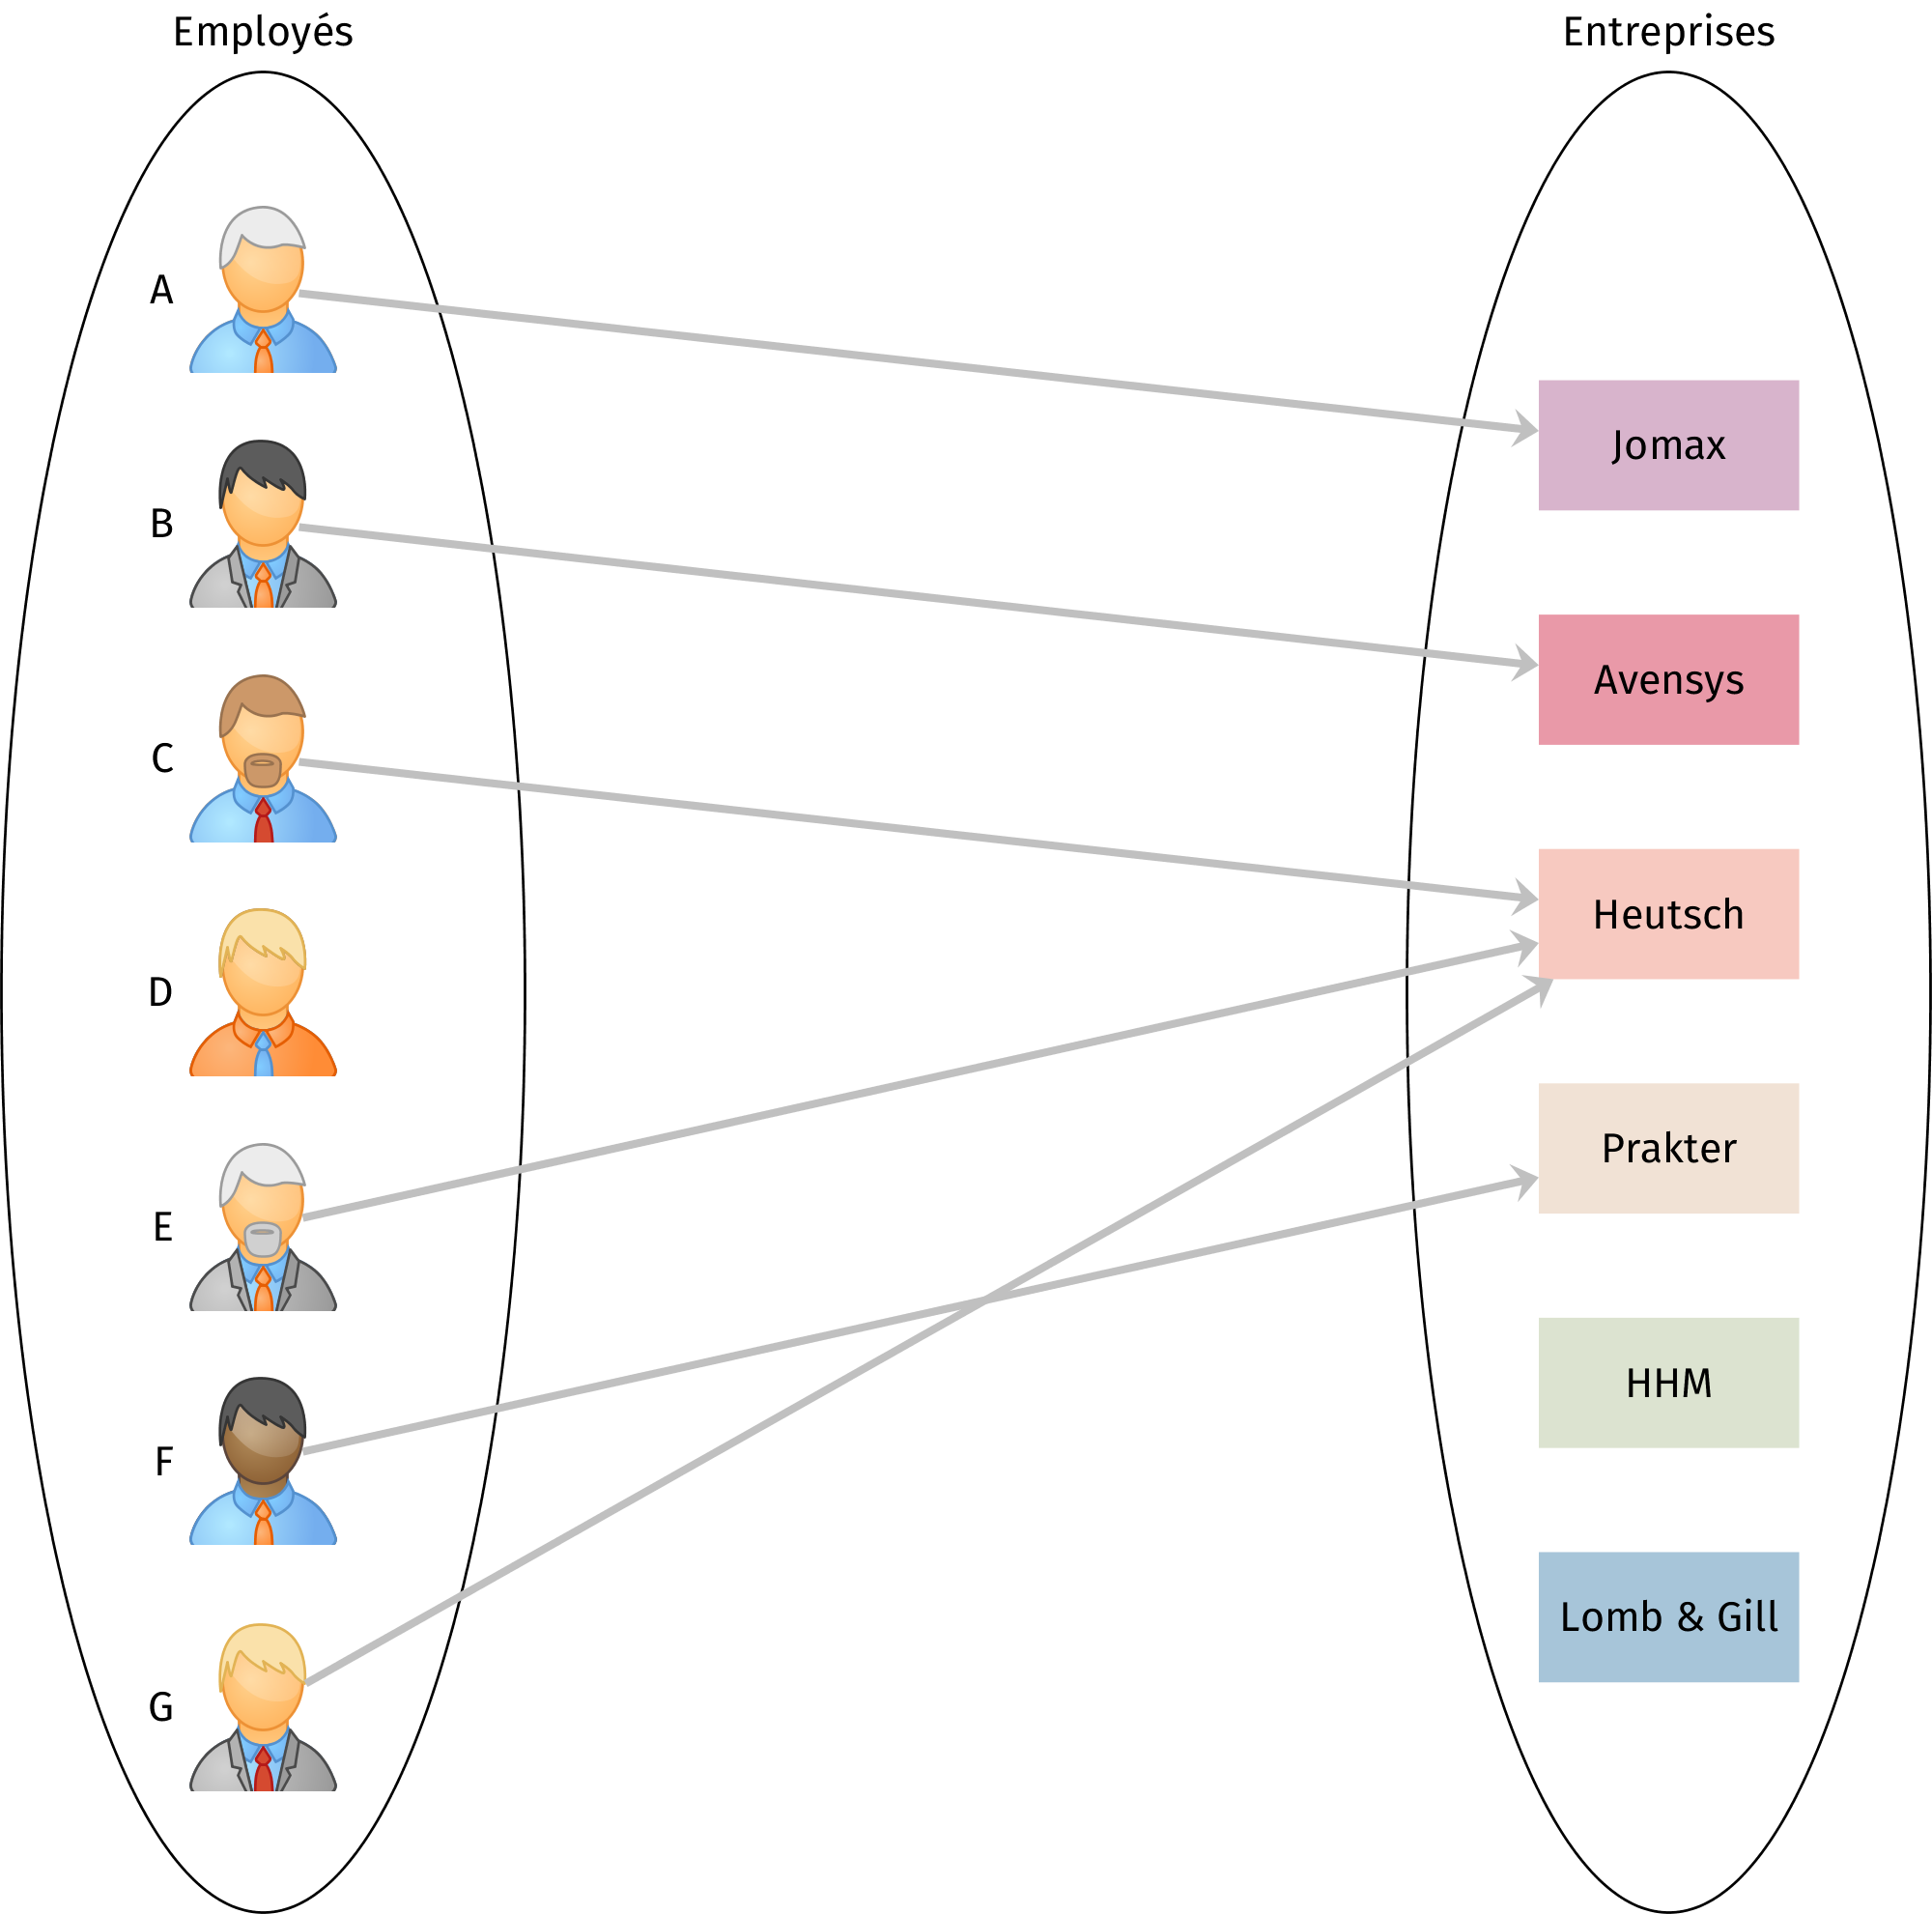
\includegraphics[width=7cm]{ensembles/img/pas_appli.png}
    \end{center}
    Celle-ci en est une car tout élément de Employés est associé à un \textit{unique} élément de Entreprises.
    \begin{center}
        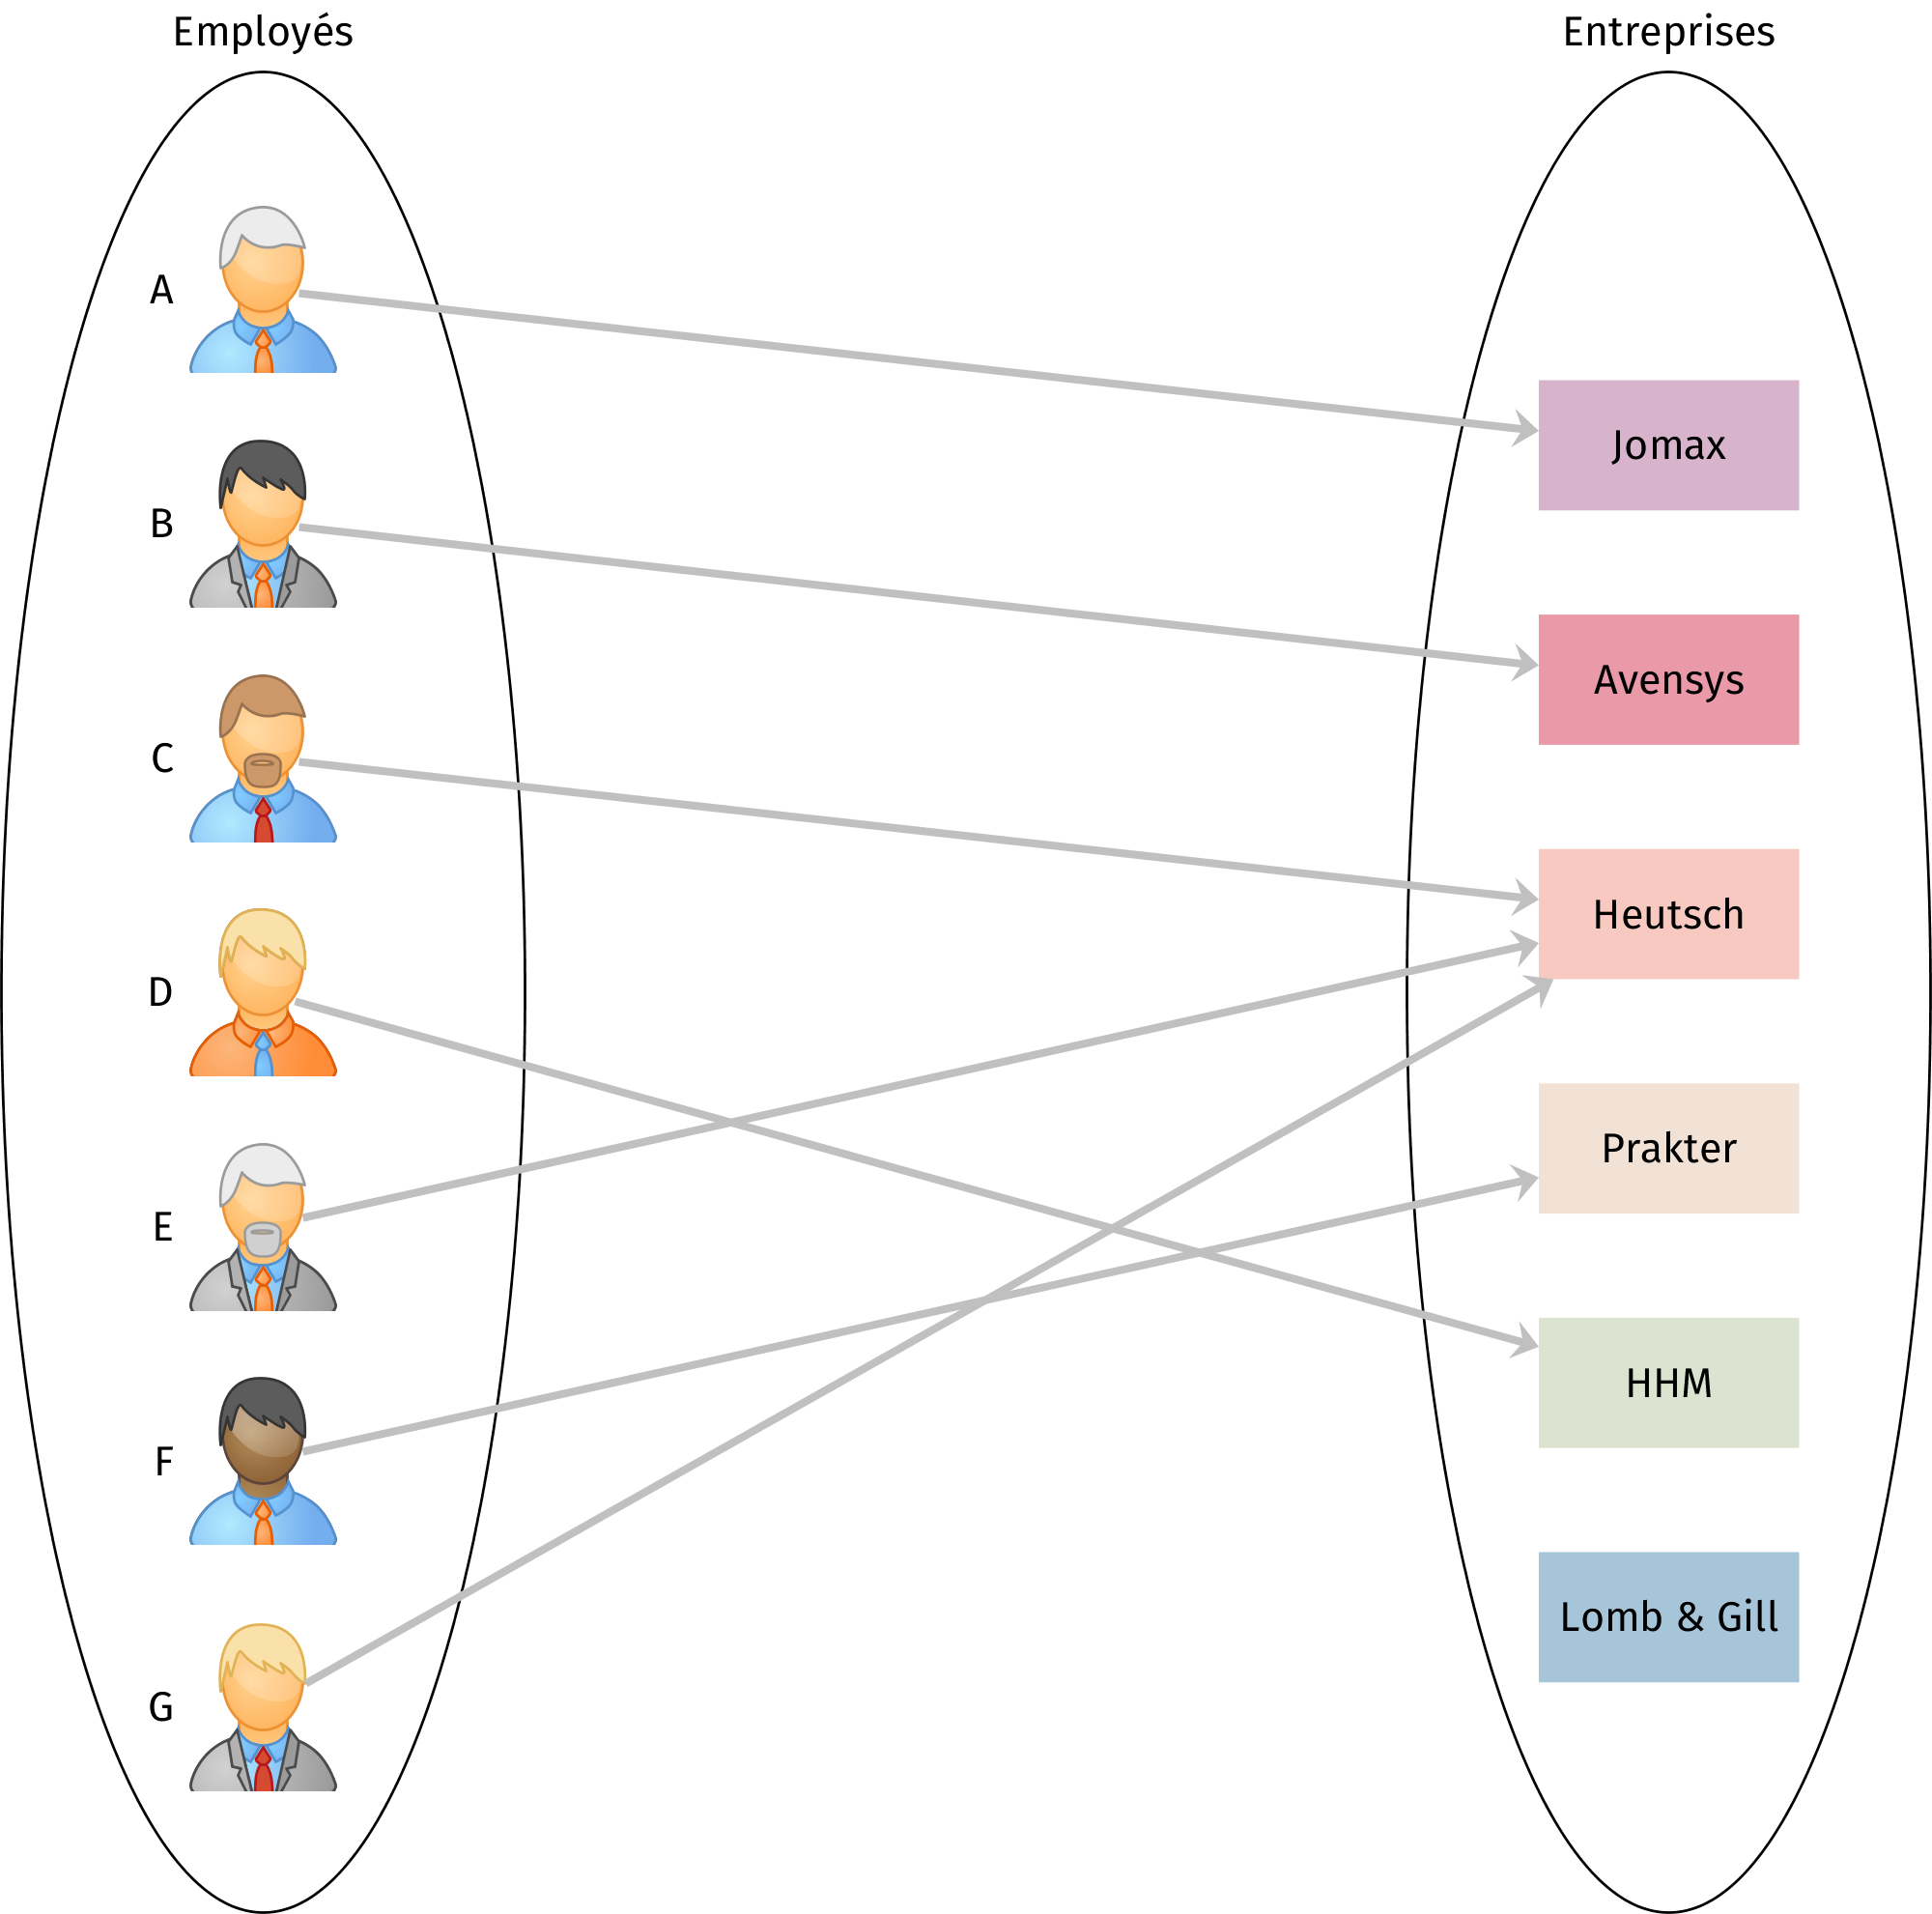
\includegraphics[width=7cm]{ensembles/img/appli.png}
    \end{center}
    Si on décide de l'appeler $f$ alors on écrira :\\$f(A)=Jomax$ et de même $f(B)=Avensys$.
\end{exemple}

\begin{remarque}[]
    Lorsque $f$ est une application de $E$ dans $F$, \textit{tous} les éléments de $E$ ont \textit{une unique image} dans $F$. En revanche, tous les éléments de l'ensemble d'arrivée $F$ n'ont pas obligatoirement un unique antécédent par $f$ : chacun peut en avoir aucun, un seul ou plusieurs.\\
    Dans l'exemple précédent Jomax admet A pour unique antécédent. Heutsch admet 3 antécédents, et Lomb \& Gill n'en a aucun.
\end{remarque}

\begin{definition}[s : injection, surjection, bijection]
    Soit $f$ une application de $E$ dans $F$.
    \begin{itemize}
        \item 	Si tout élément de $F$ admet \textit{au plus} un antécédent par $f$ alors on dit que $f$ est \textit{injective} ou bien que c'est une \textit{injection}.
              \begin{center}
                  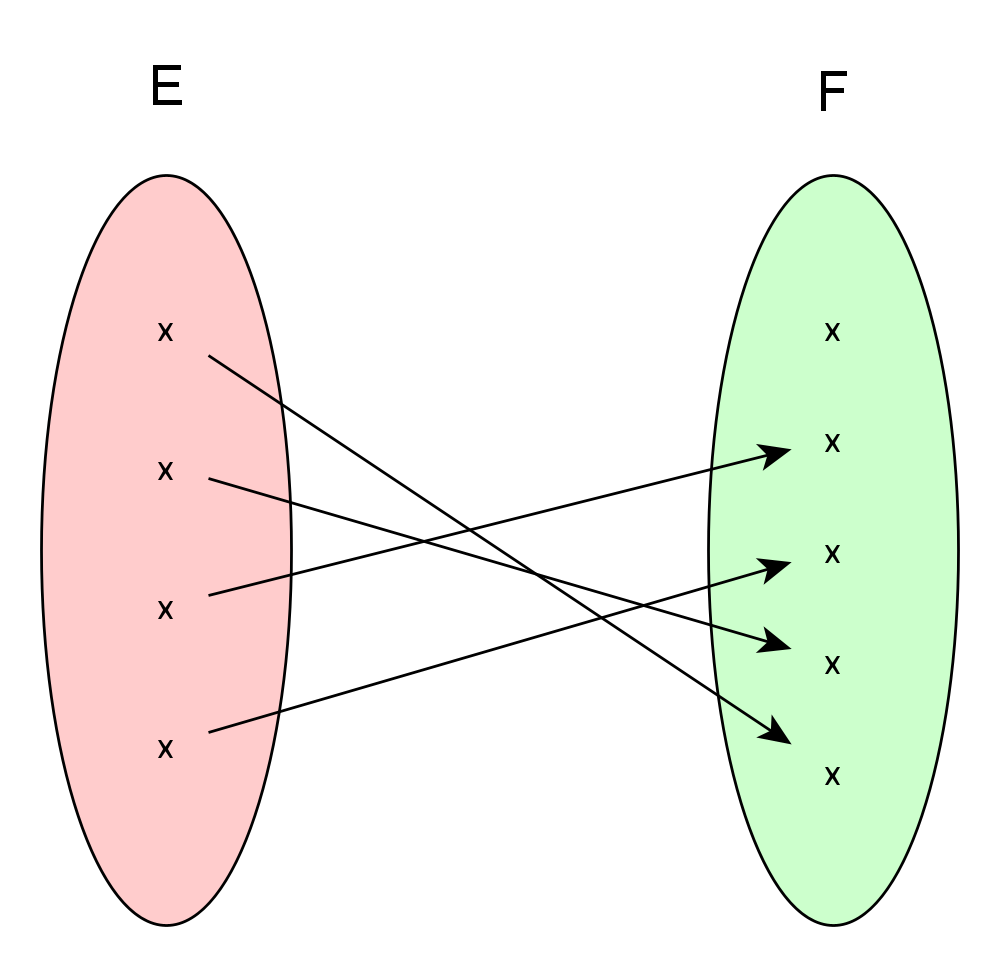
\includegraphics[width=6cm]{ensembles/img/ex_inj.png}\\ {\footnotesize injection de $E$ dans $F$}
              \end{center}
        \item 	Si tout élément de $F$ admet \textit{au moins} un antécédent par $f$ alors on dit que $f$ est \textit{surjective} ou bien que c'est une \textit{surjection}.
              \begin{center}
                  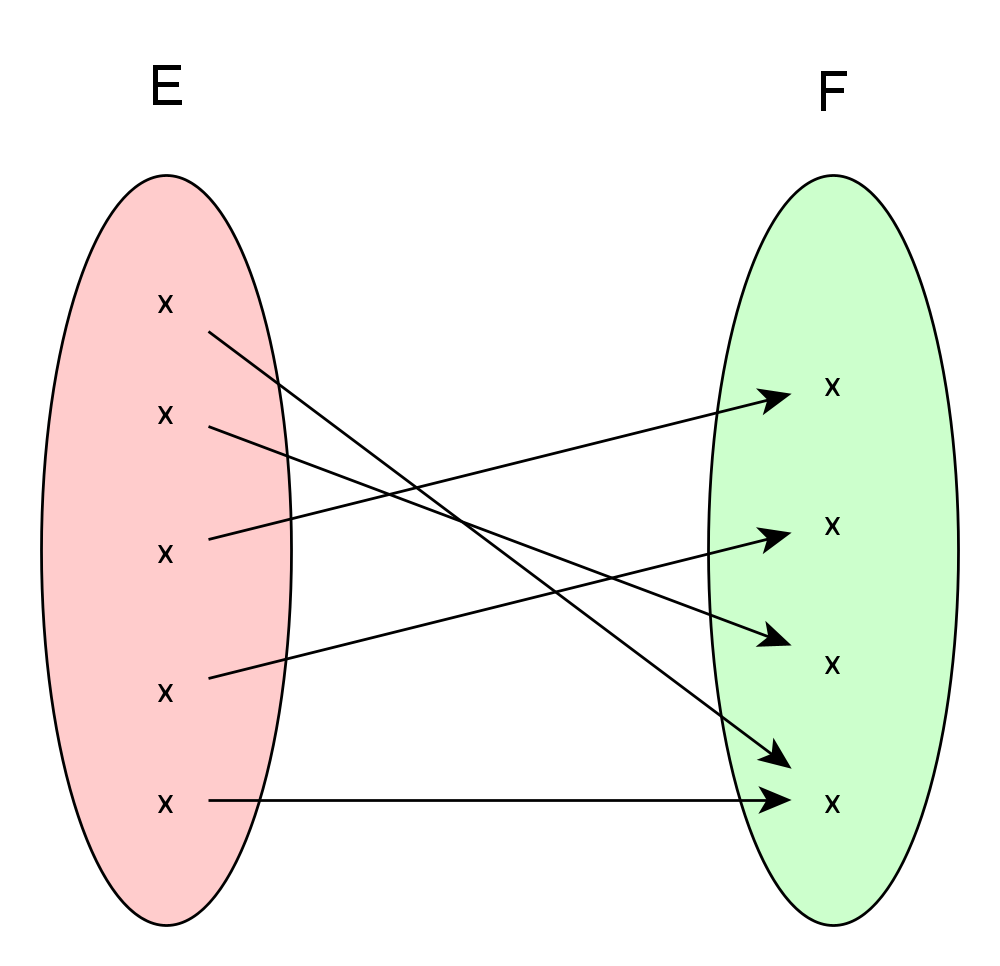
\includegraphics[width=6cm]{ensembles/img/ex_surj.png}\\ {\footnotesize surjection de $E$ dans $F$}
              \end{center}
        \item tout élément de $F$ admet \textit{exactement} un antécédent par $f$ alors  $f$ est \textit{à la fois injective et surjective} et on dit que $f$ est \textit{bijective} ou bien que c'est une \textit{bijection}.
              \begin{center}
                  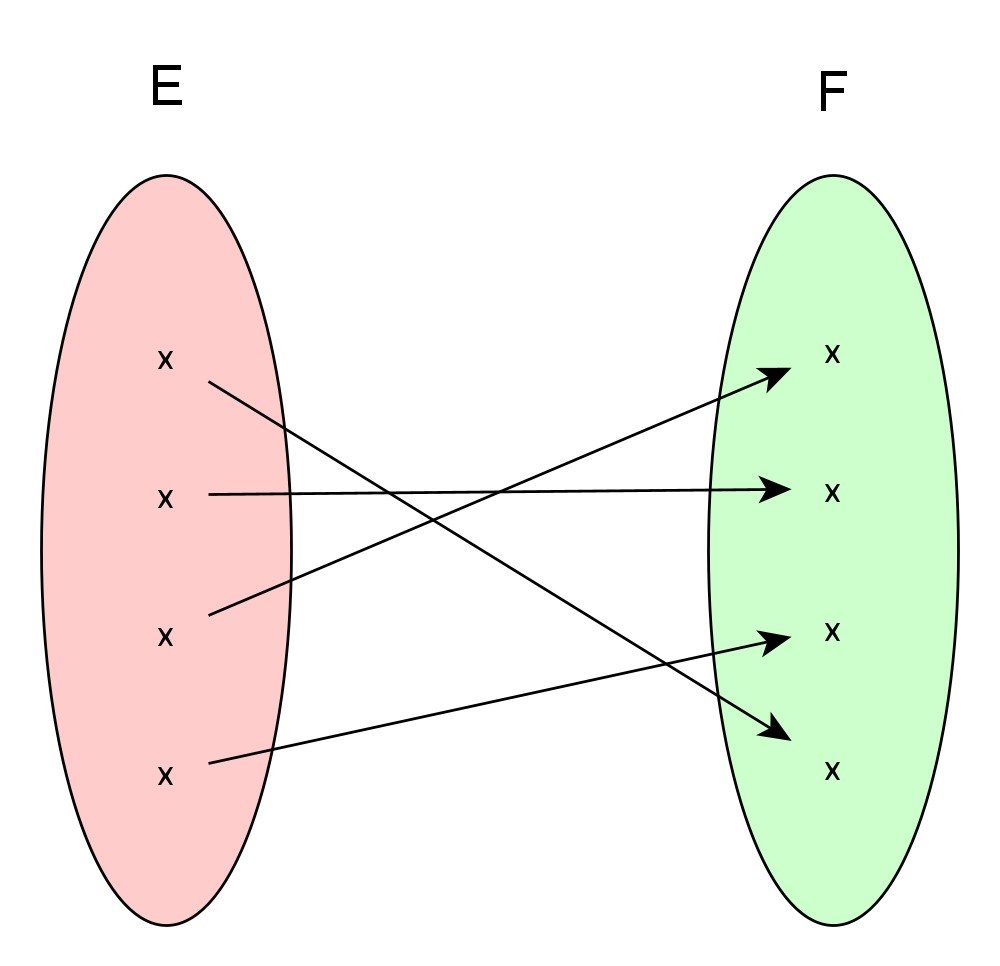
\includegraphics[width=6cm]{ensembles/img/ex_bij.png}\\ {\footnotesize bijection de $E$ dans $F$}
              \end{center}
    \end{itemize}
\end{definition}


\begin{exercice}[]
    Pour chaque relation de E (en rose à gauche) vers F (en vert à droite) indiquer si c'est une application, et si elle est injective, surjective, bijective ou rien du tout.
    \def\myw{5cm}
    \begin{multicols}{2}
        \begin{enumerate}
            \item 	\ \\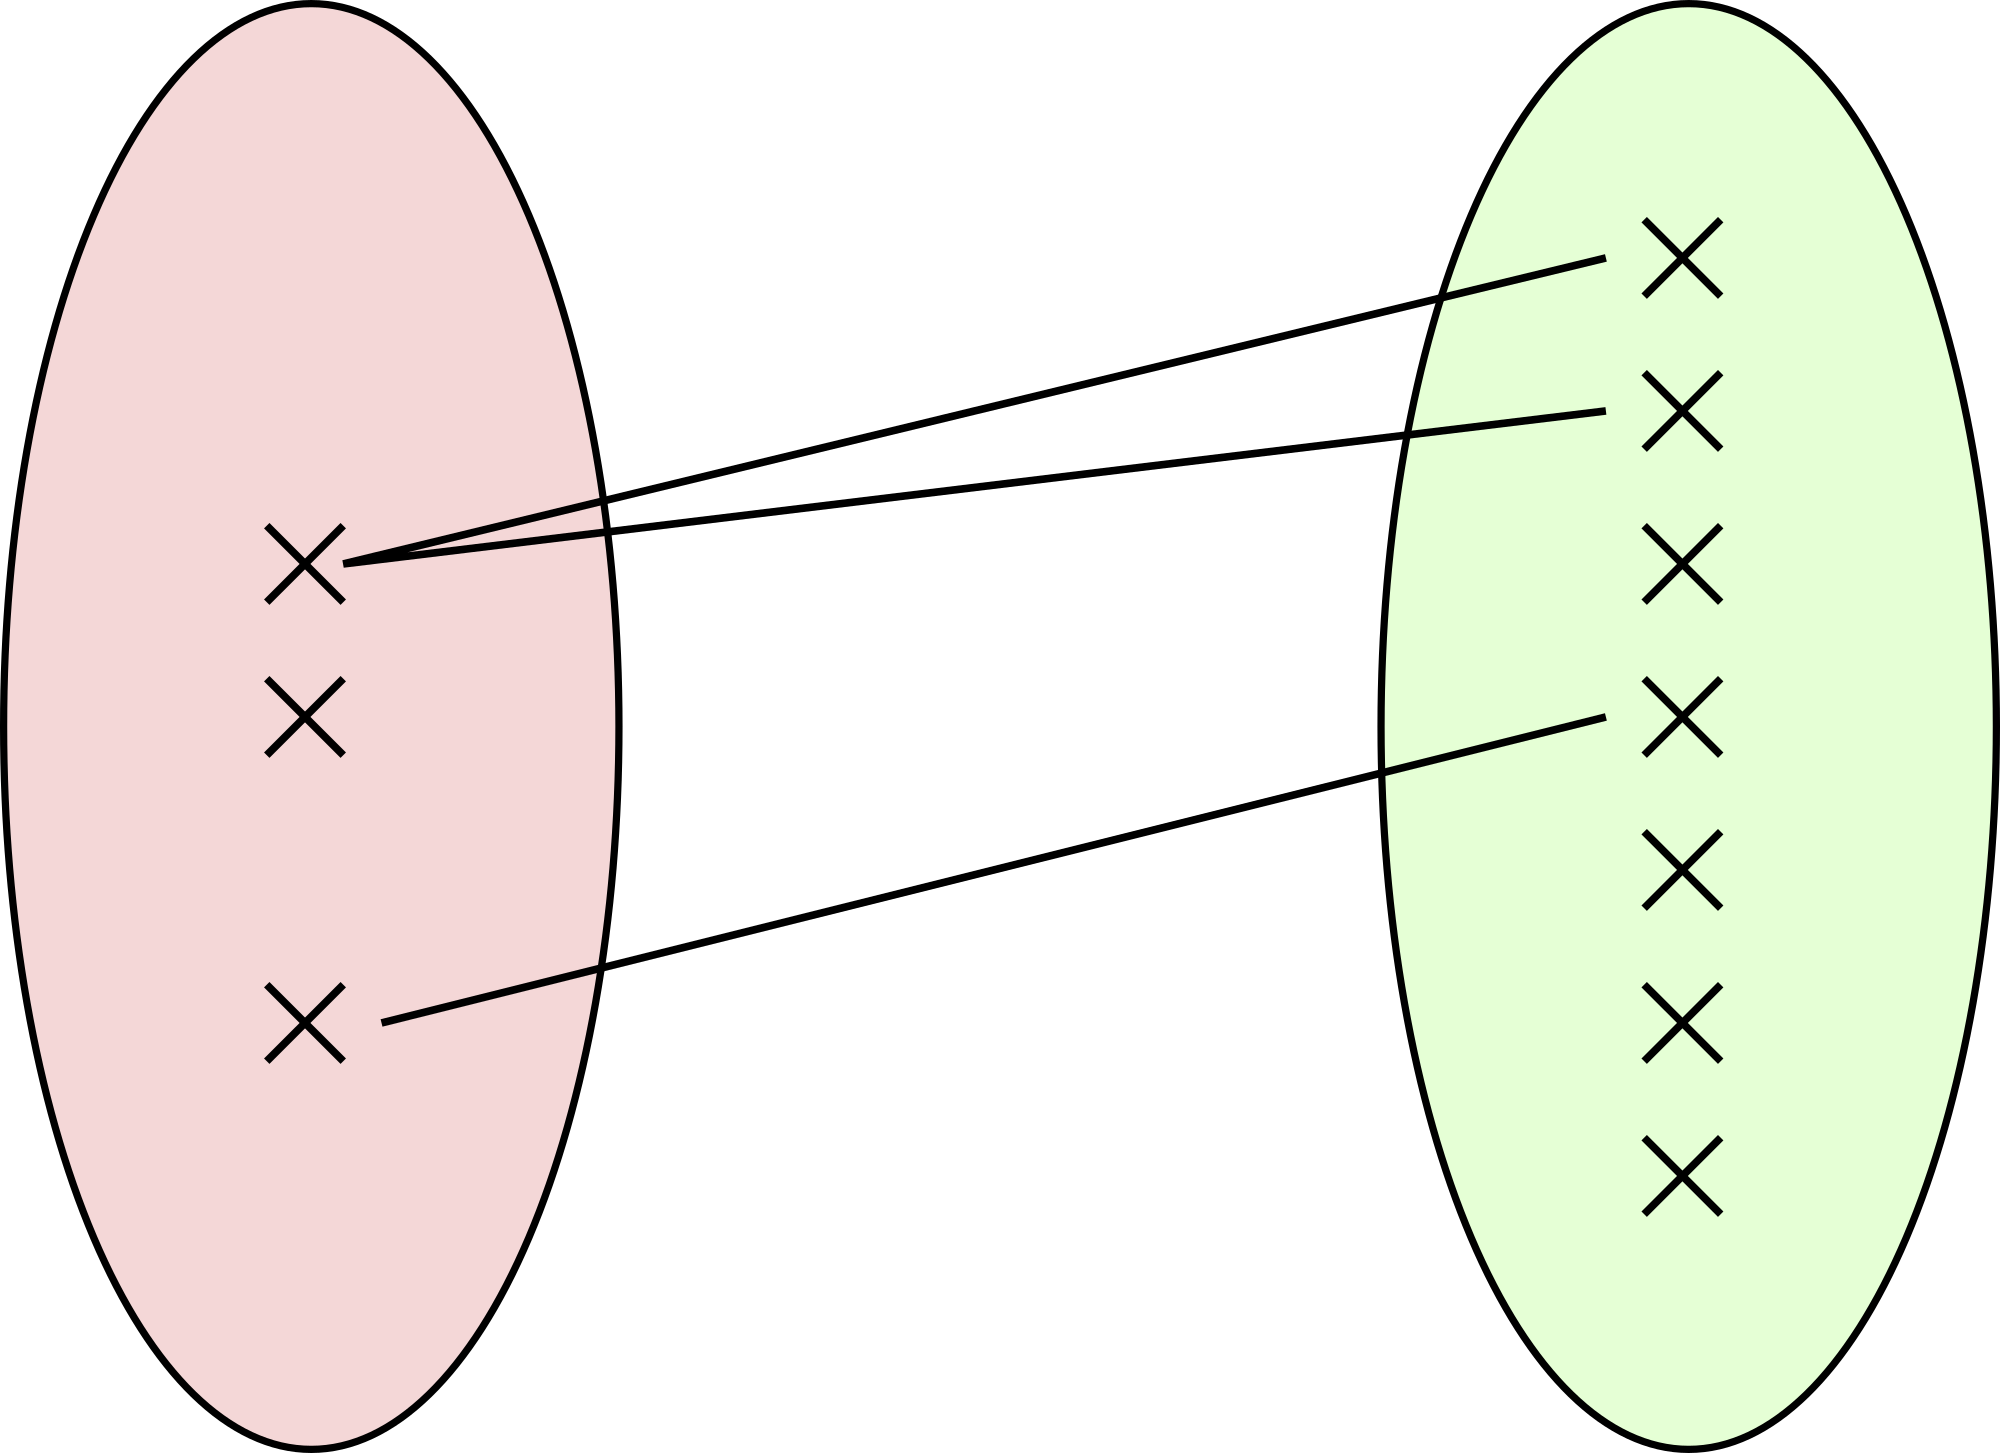
\includegraphics[width=\myw]{ensembles/img/1.png}
            \item 	\ \\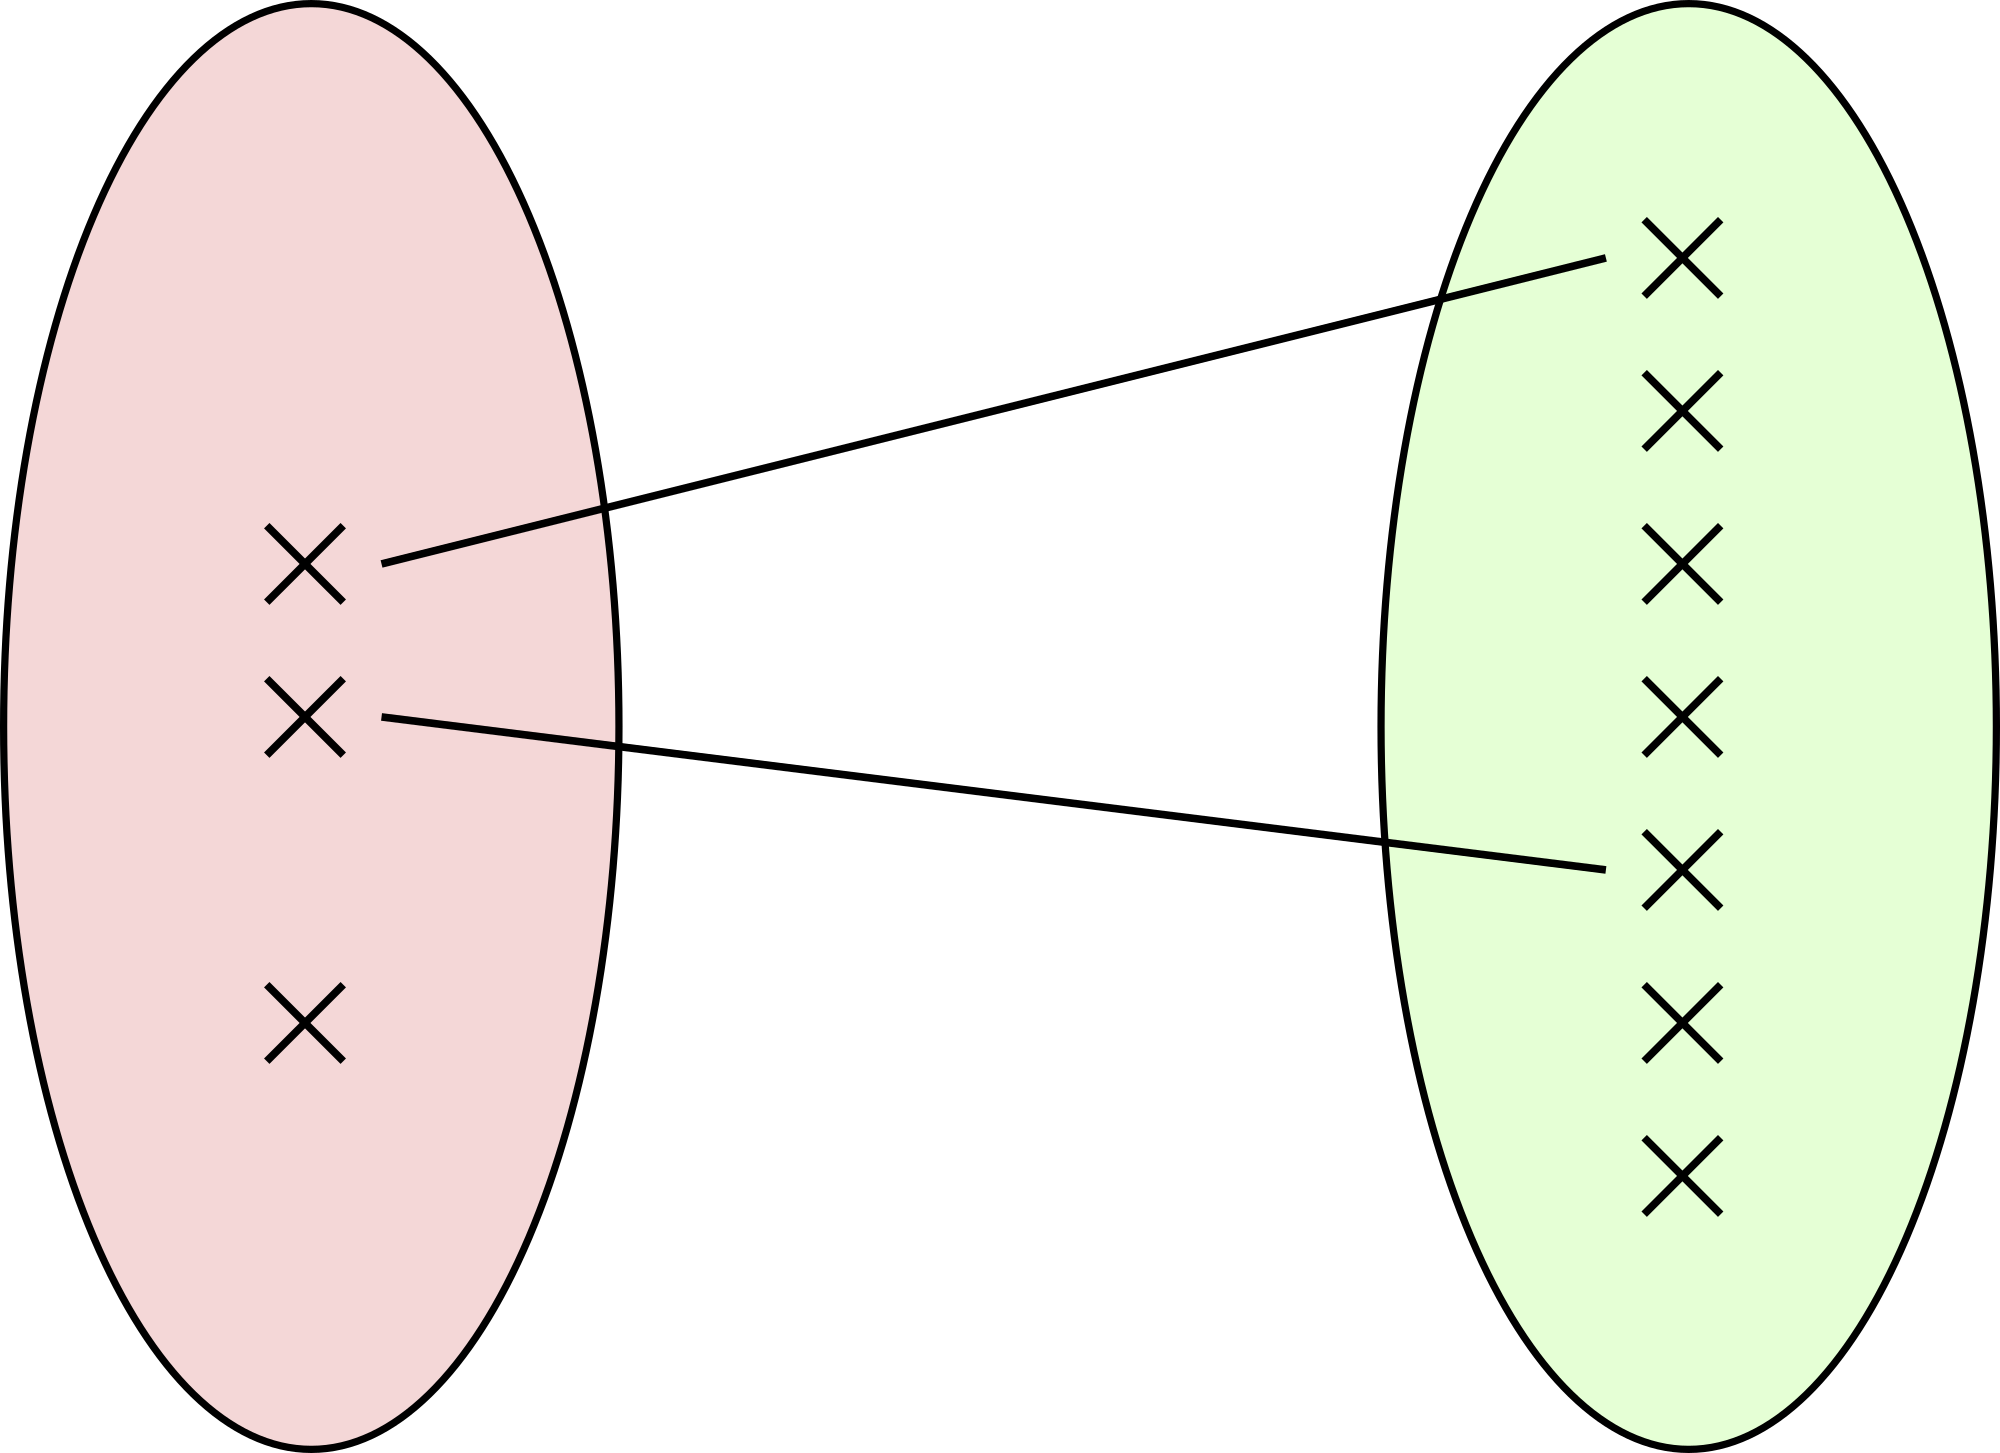
\includegraphics[width=\myw]{ensembles/img/2.png}
            \item 	\ \\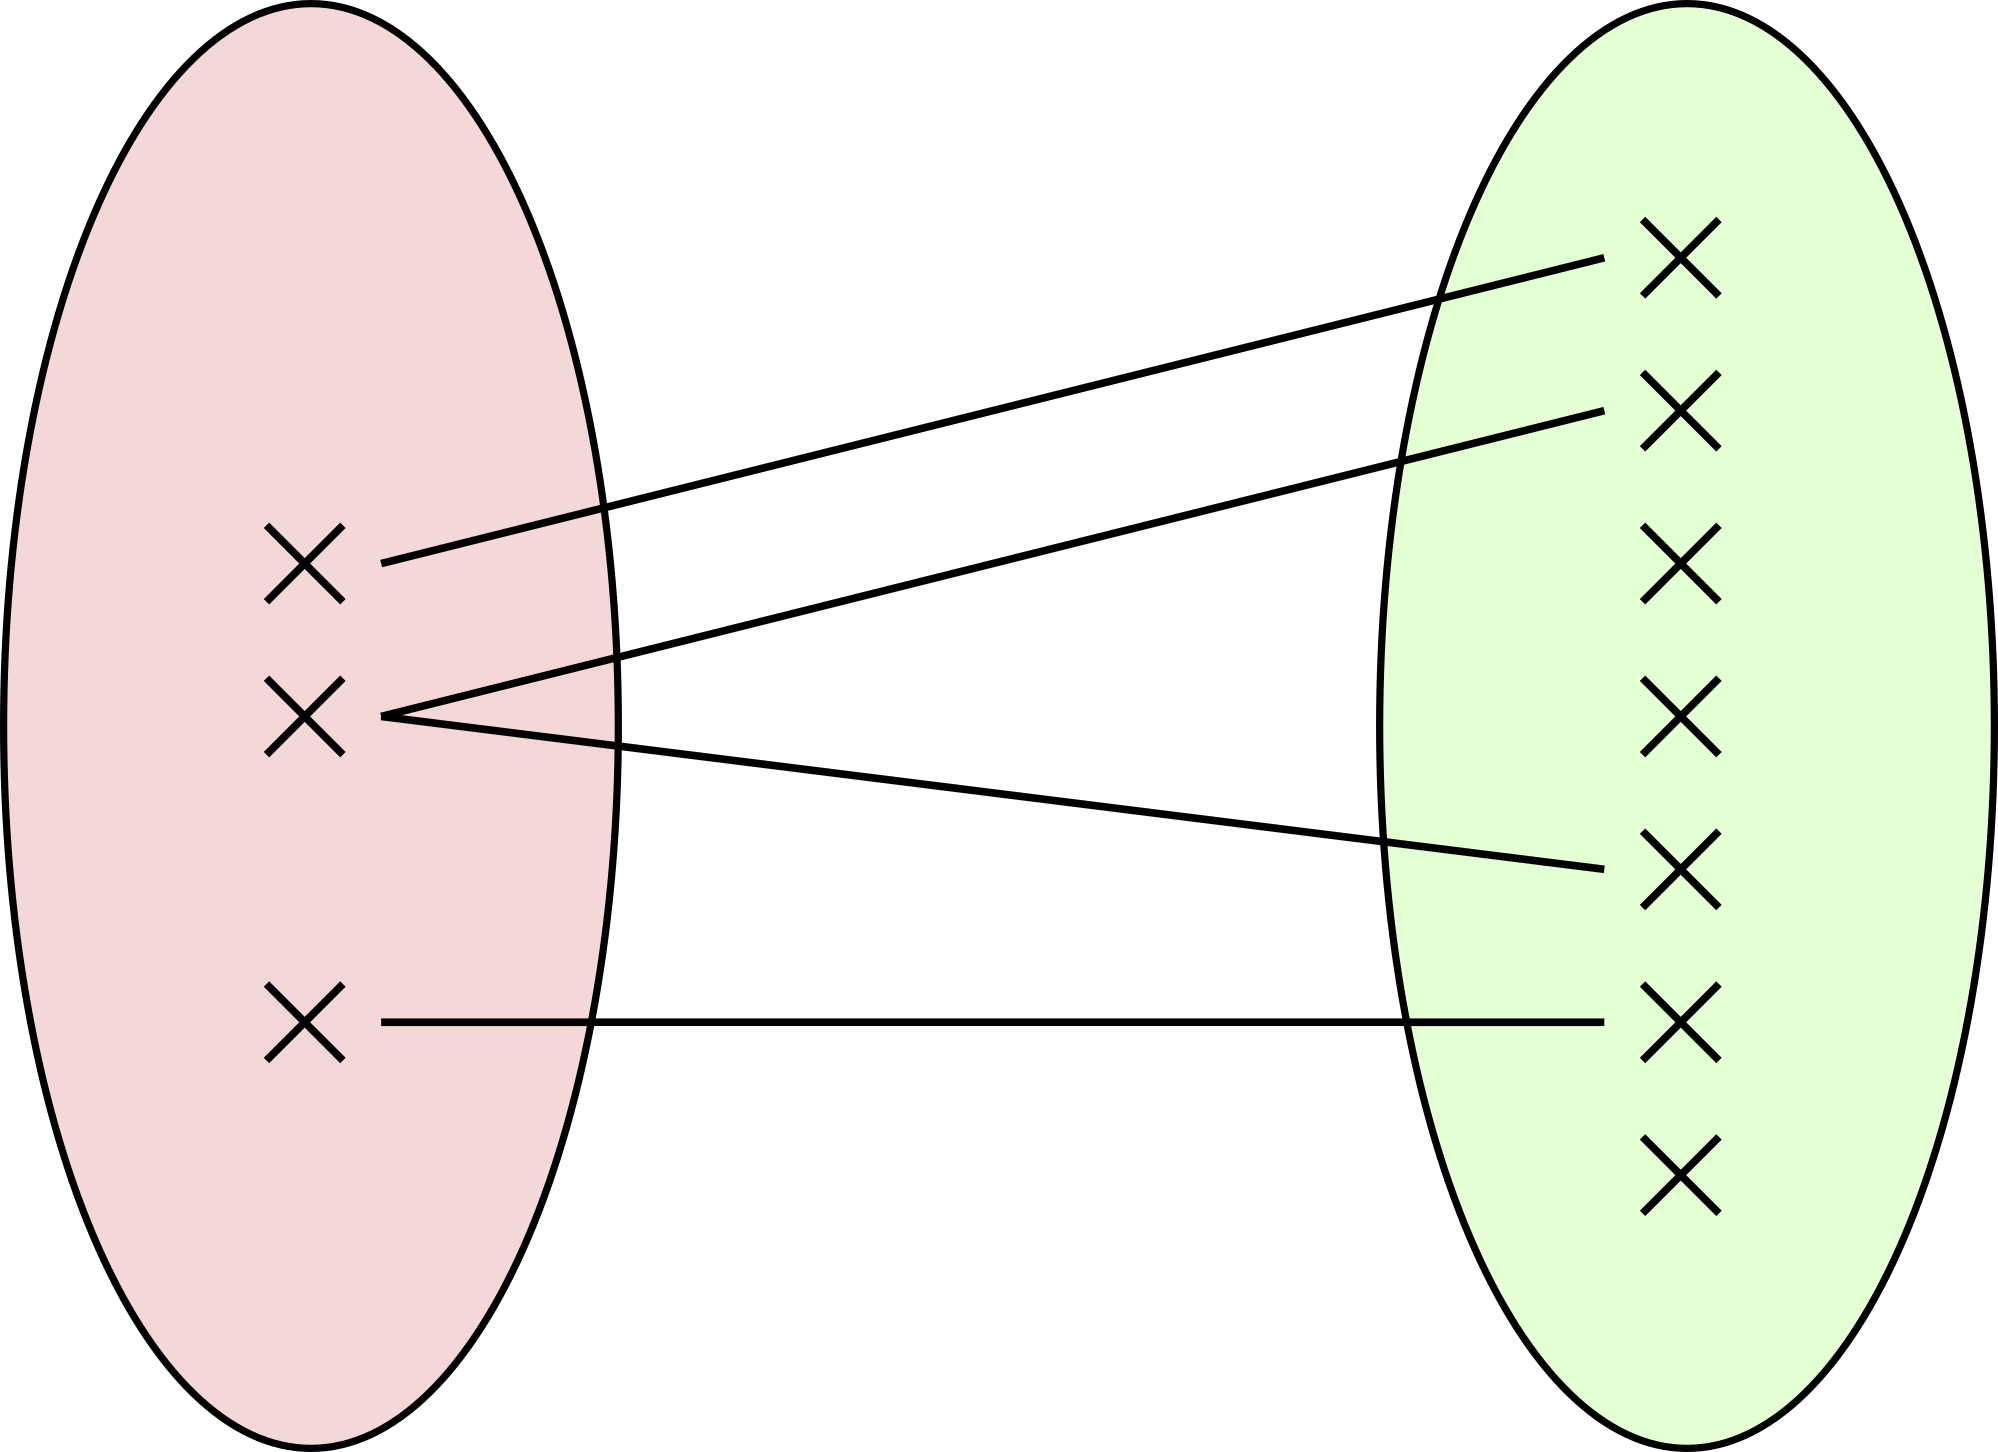
\includegraphics[width=\myw]{ensembles/img/3.png}
            \item 	\ \\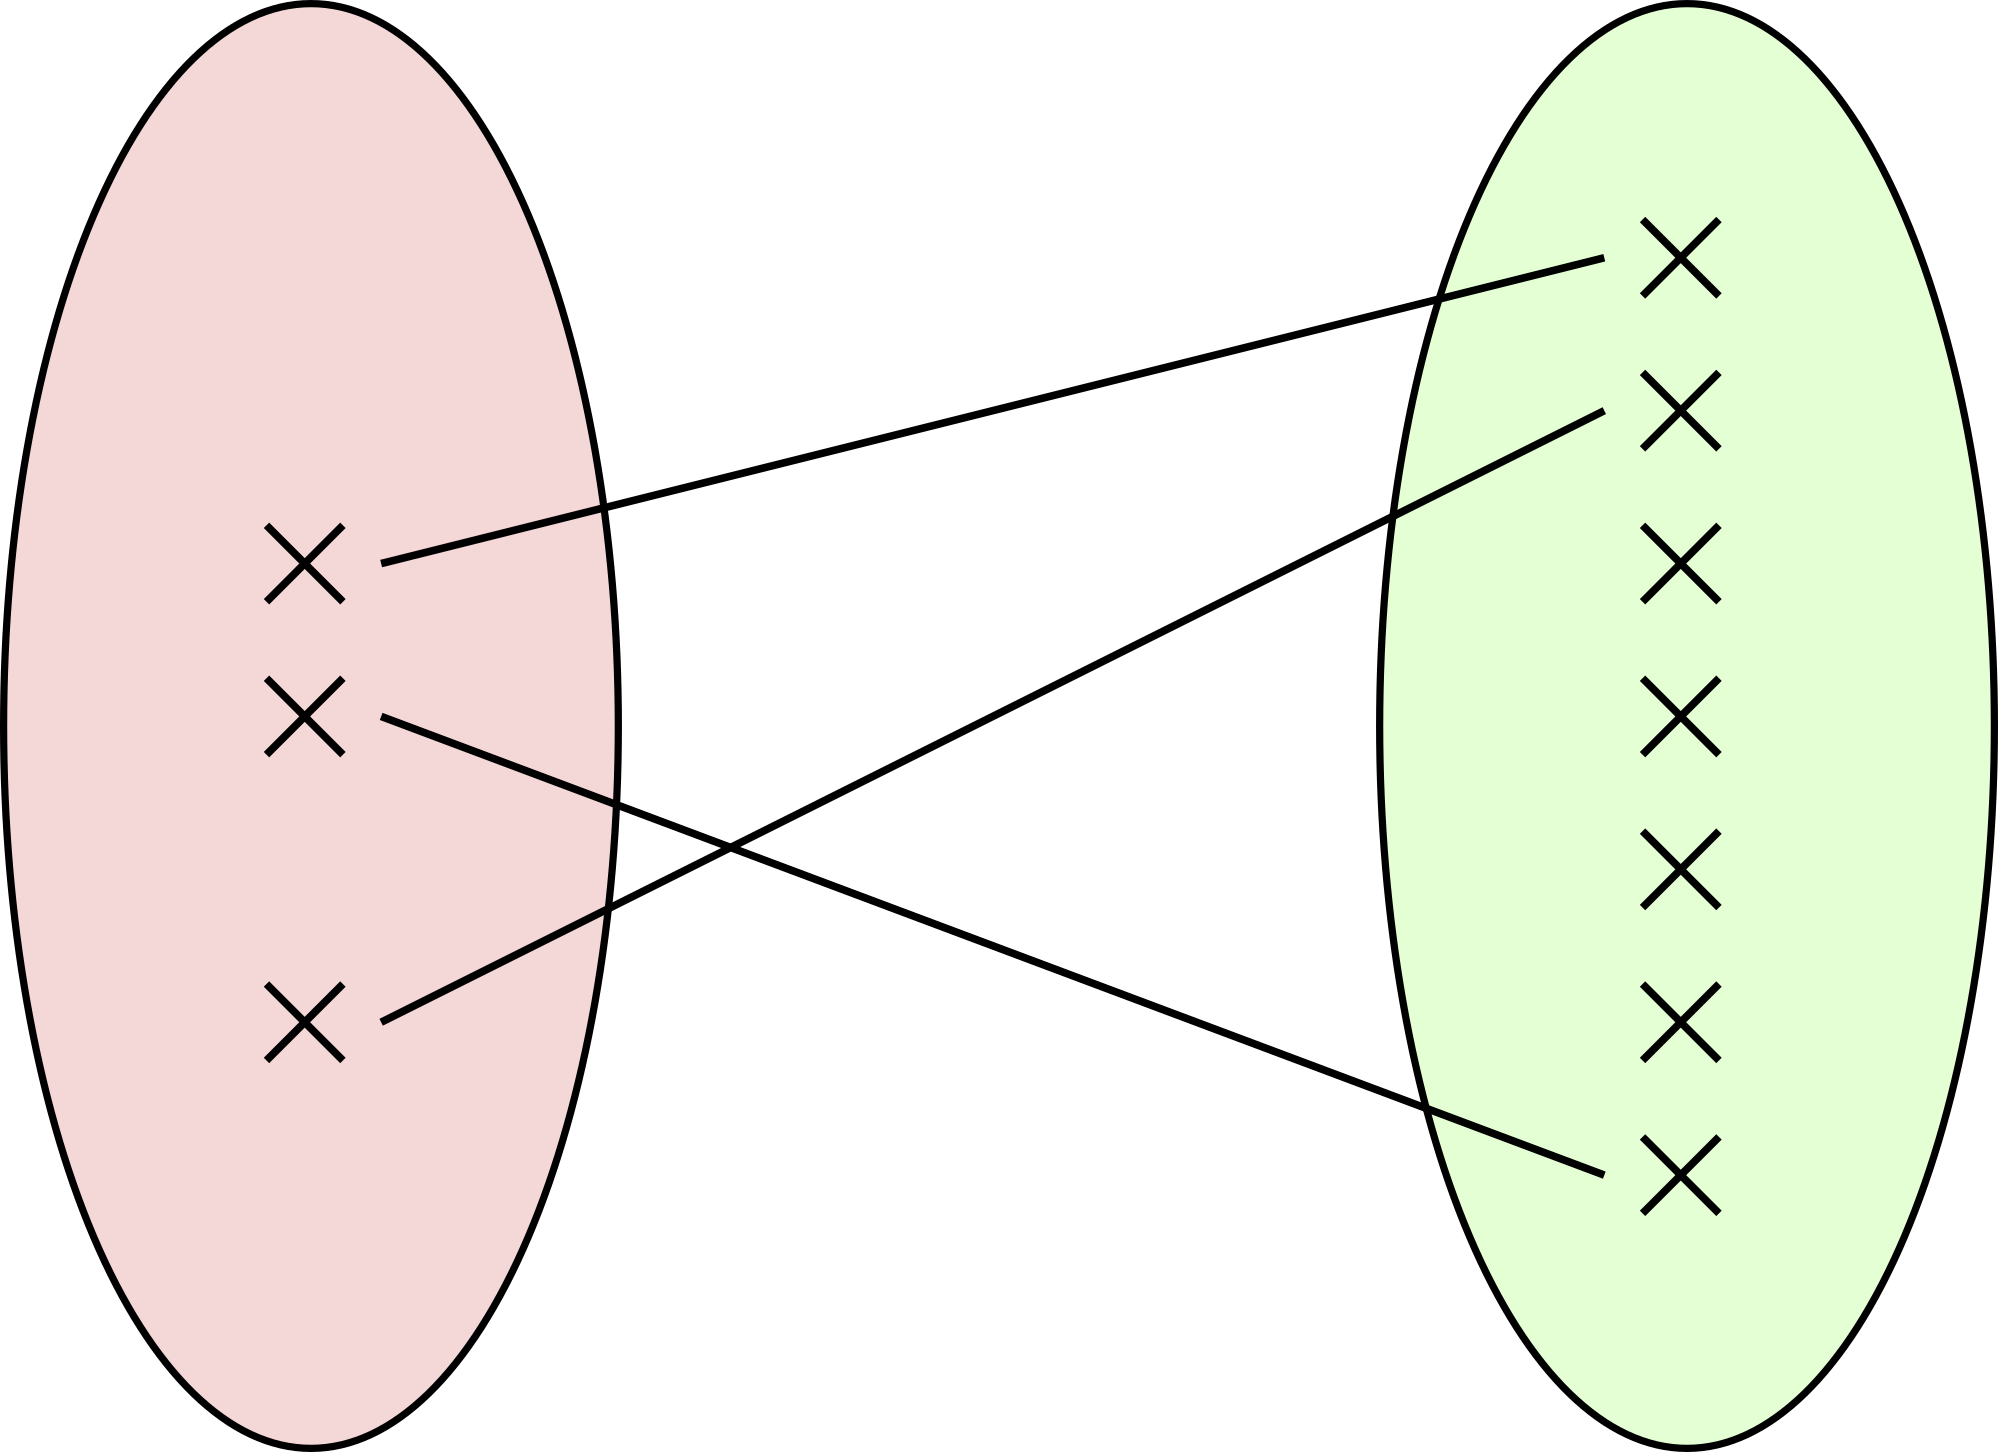
\includegraphics[width=\myw]{ensembles/img/4.png}
            \item 	\ \\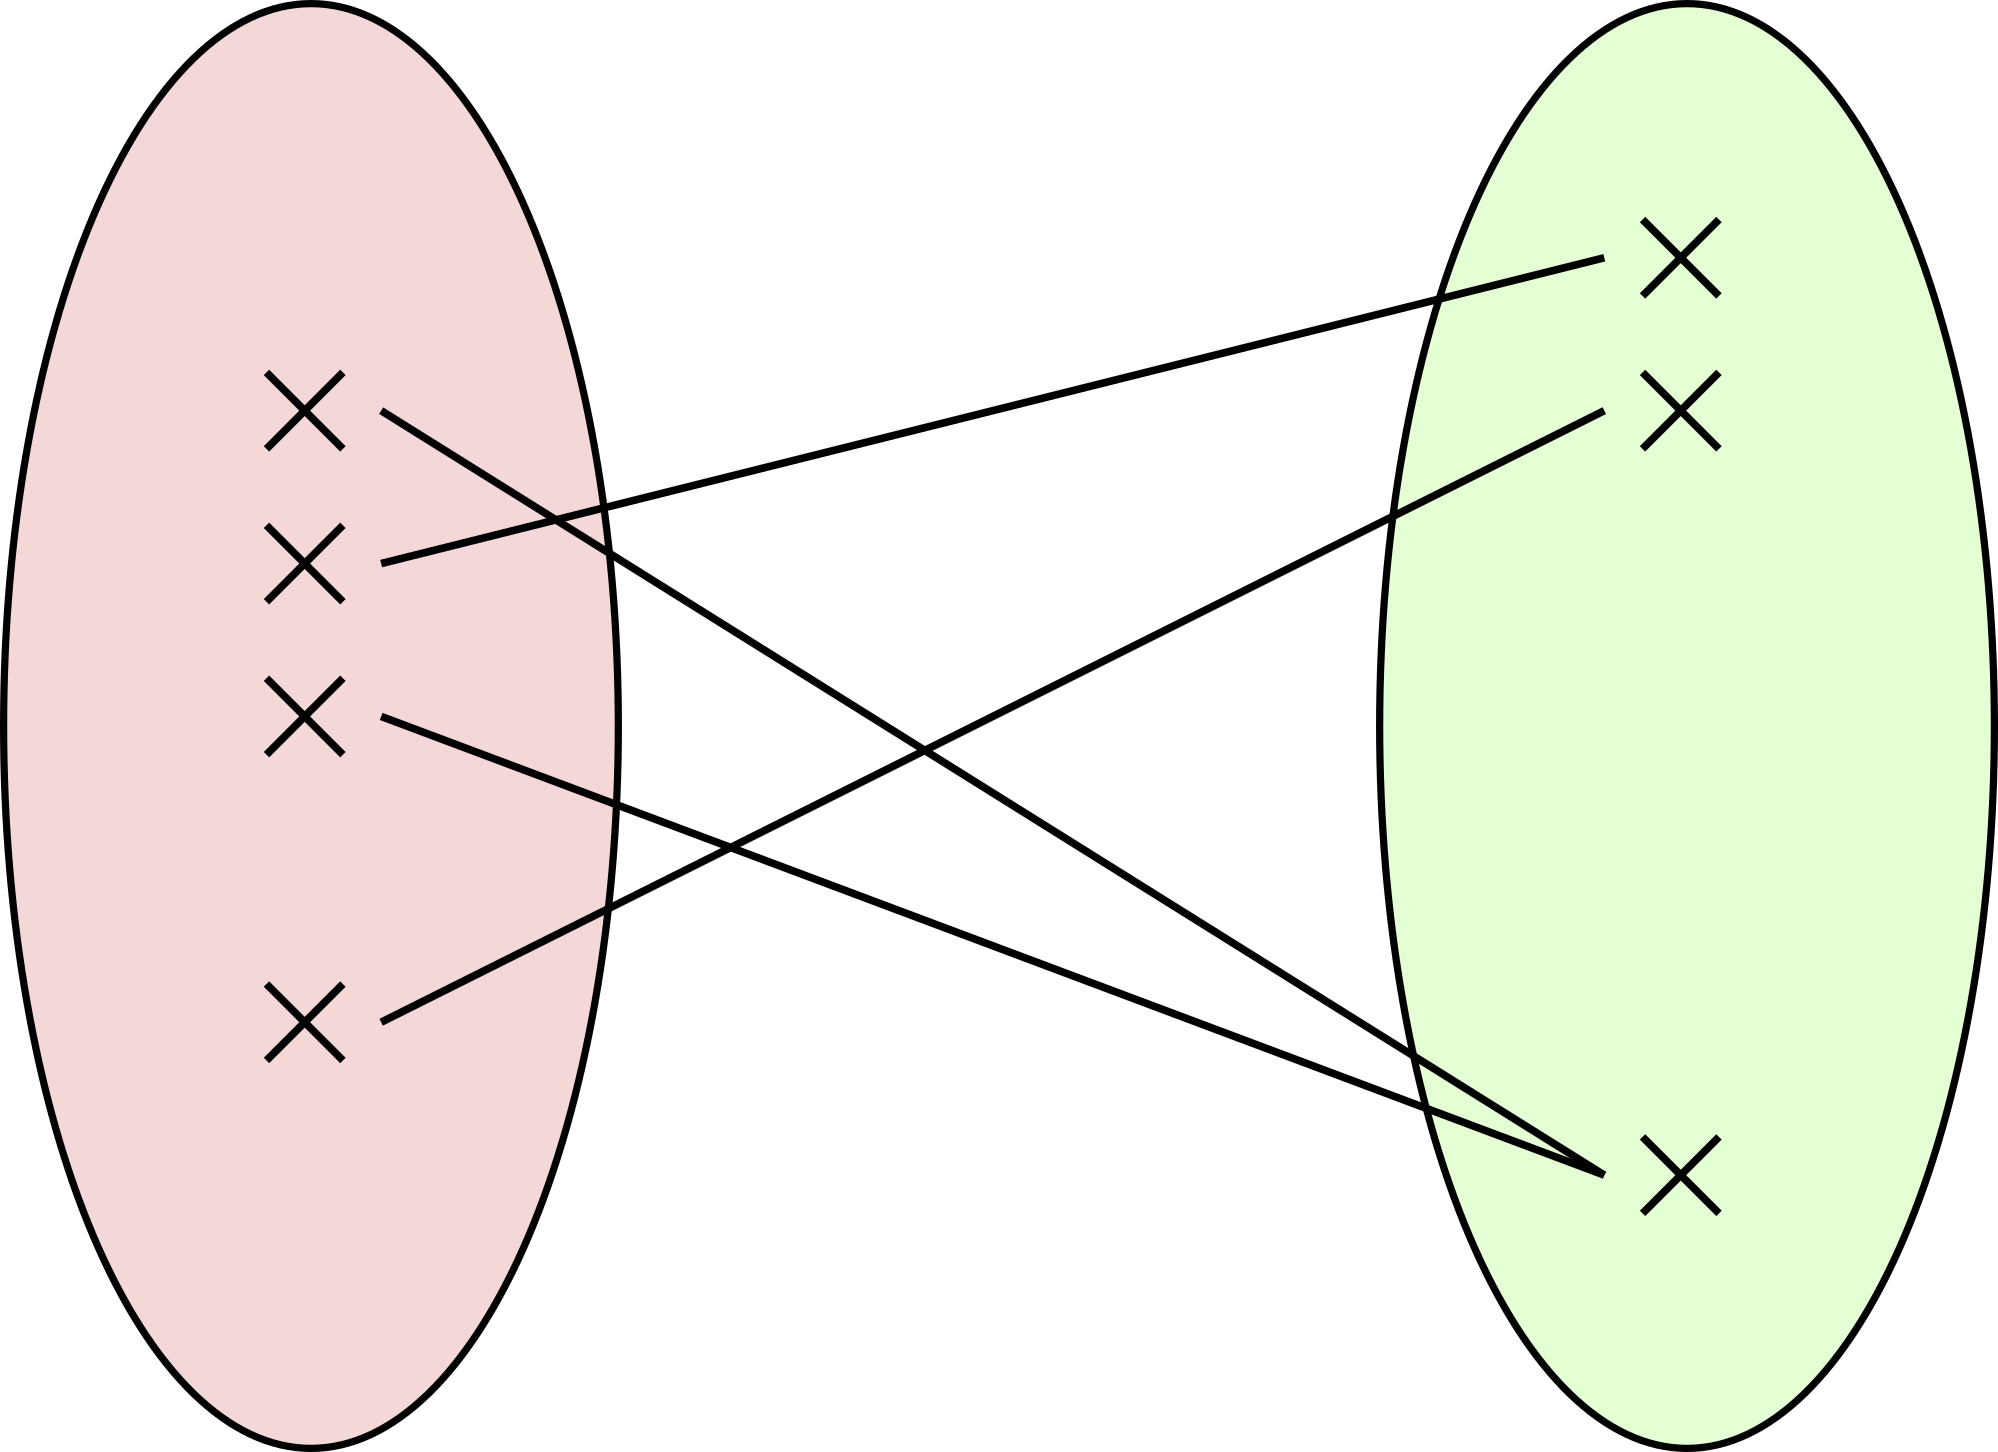
\includegraphics[width=\myw]{ensembles/img/5.png}
            \item 	\ \\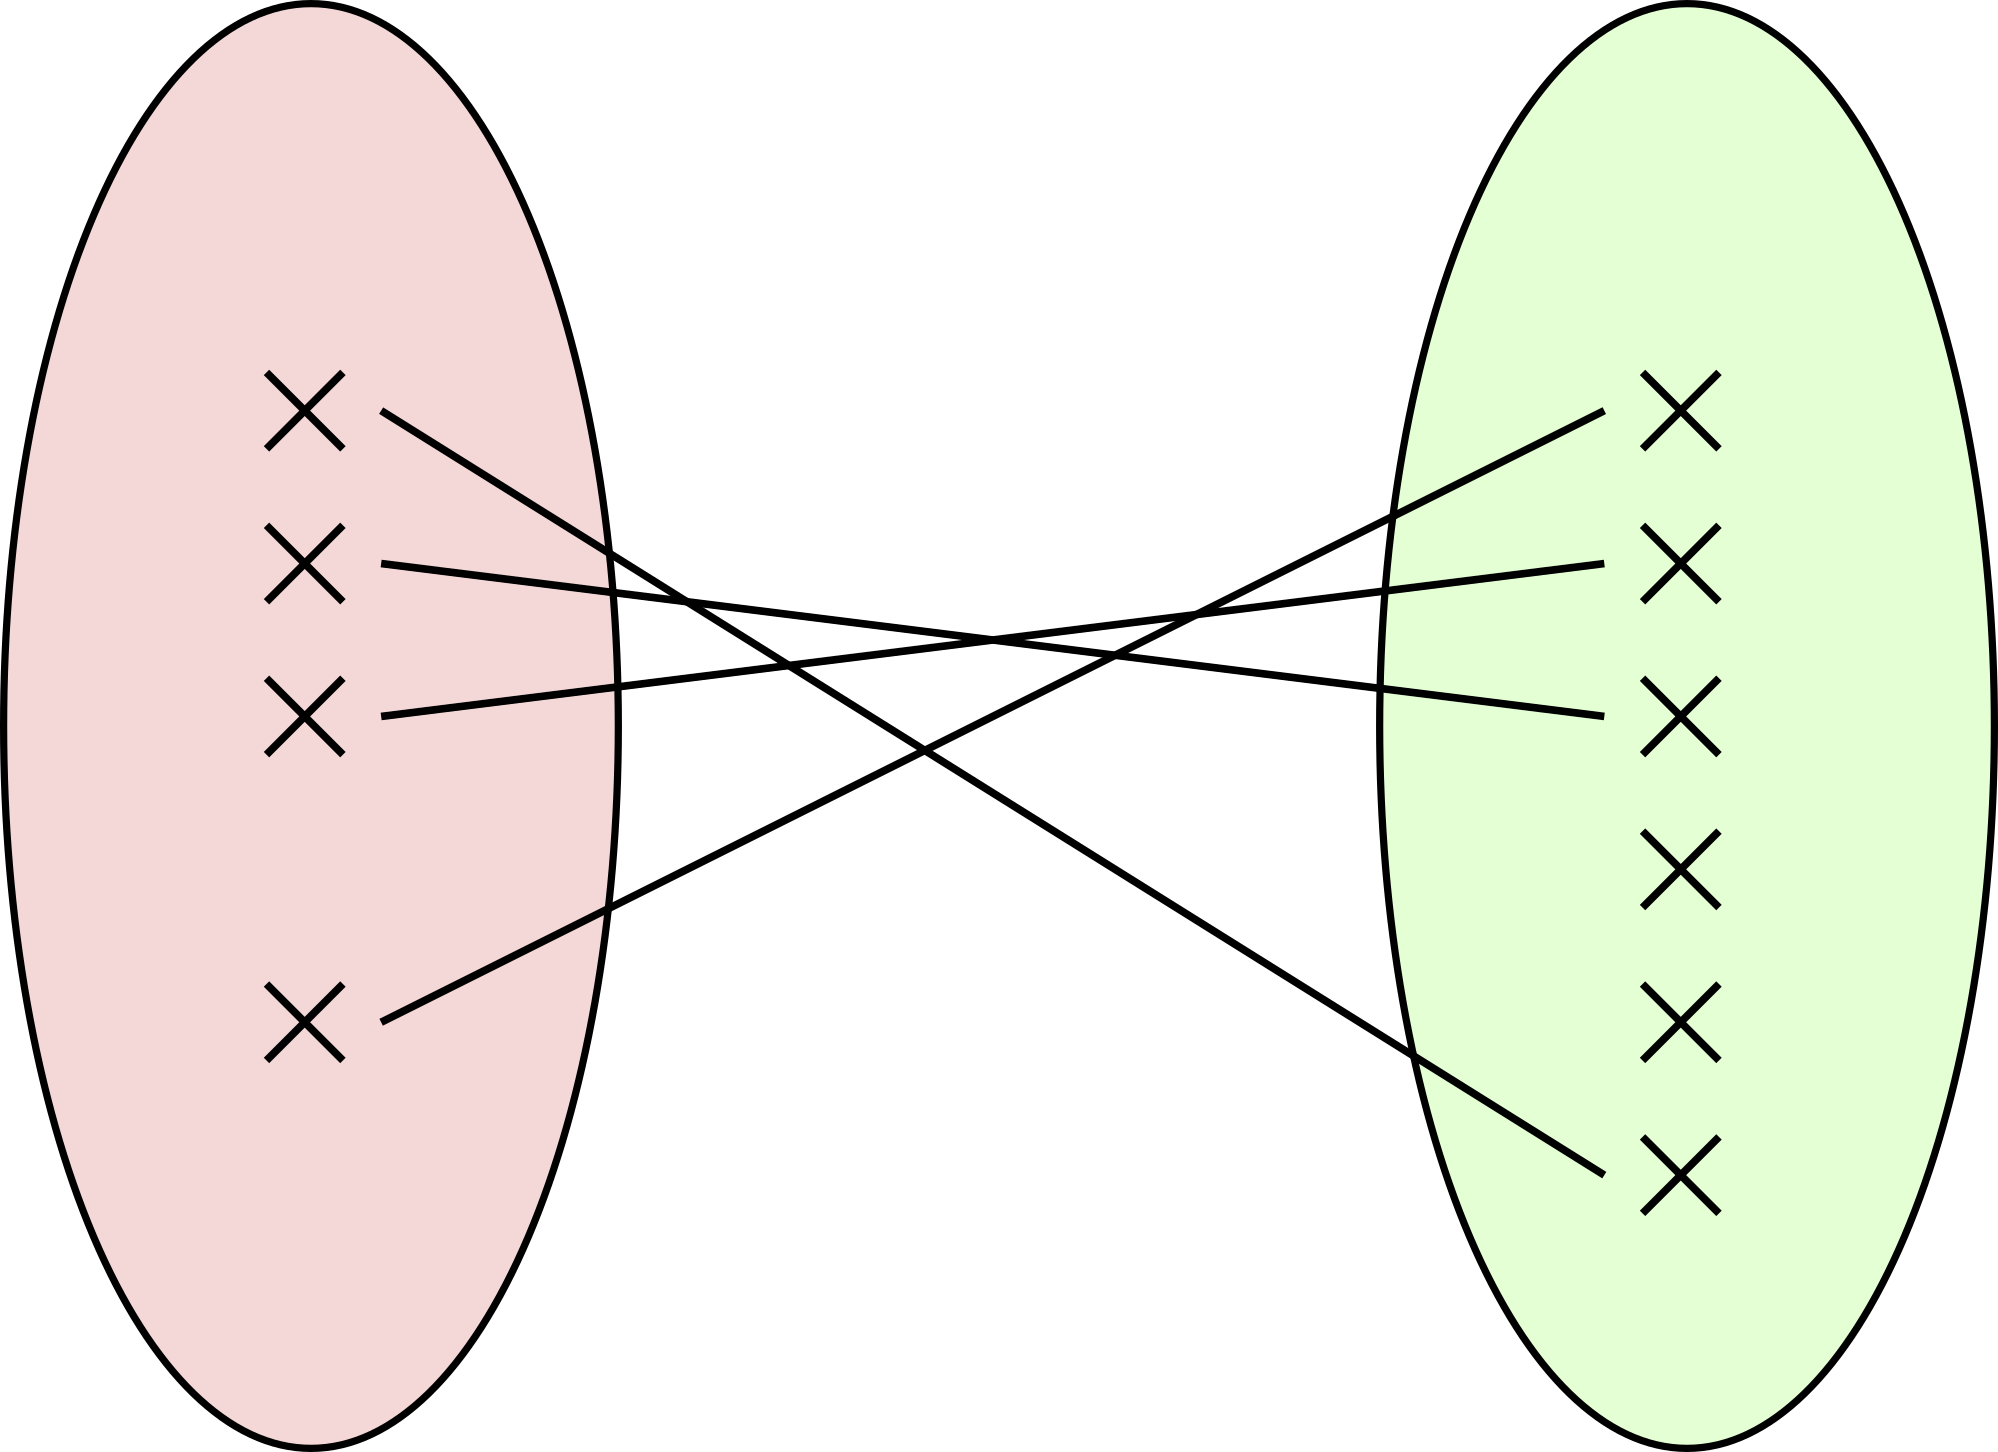
\includegraphics[width=\myw]{ensembles/img/6.png}
            \item 	\ \\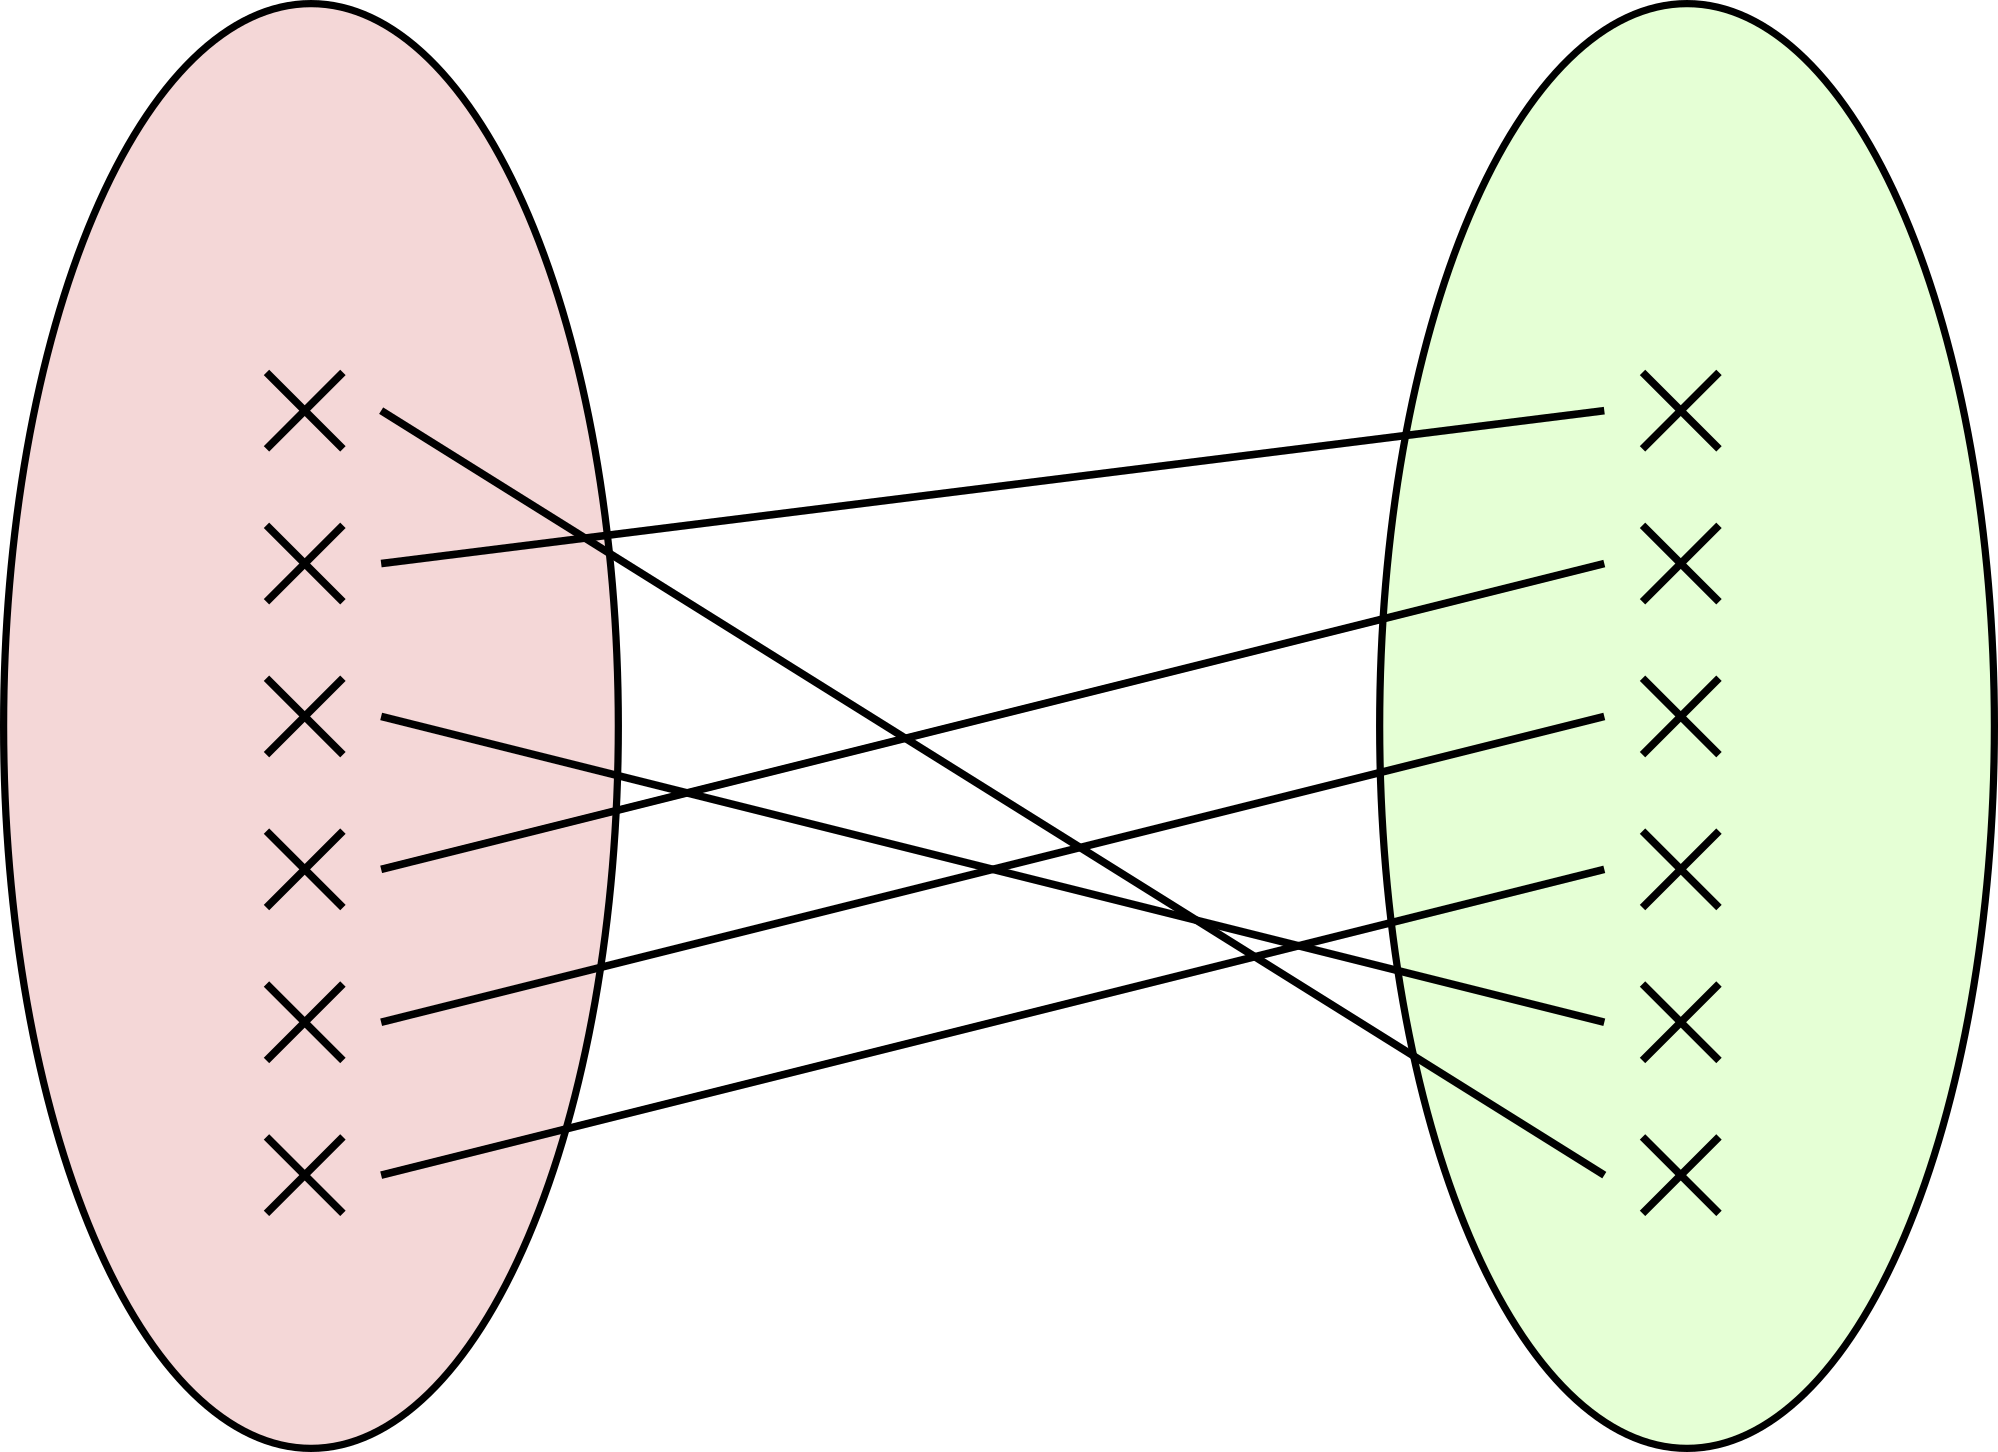
\includegraphics[width=\myw]{ensembles/img/7.png}
            \item 	\ \\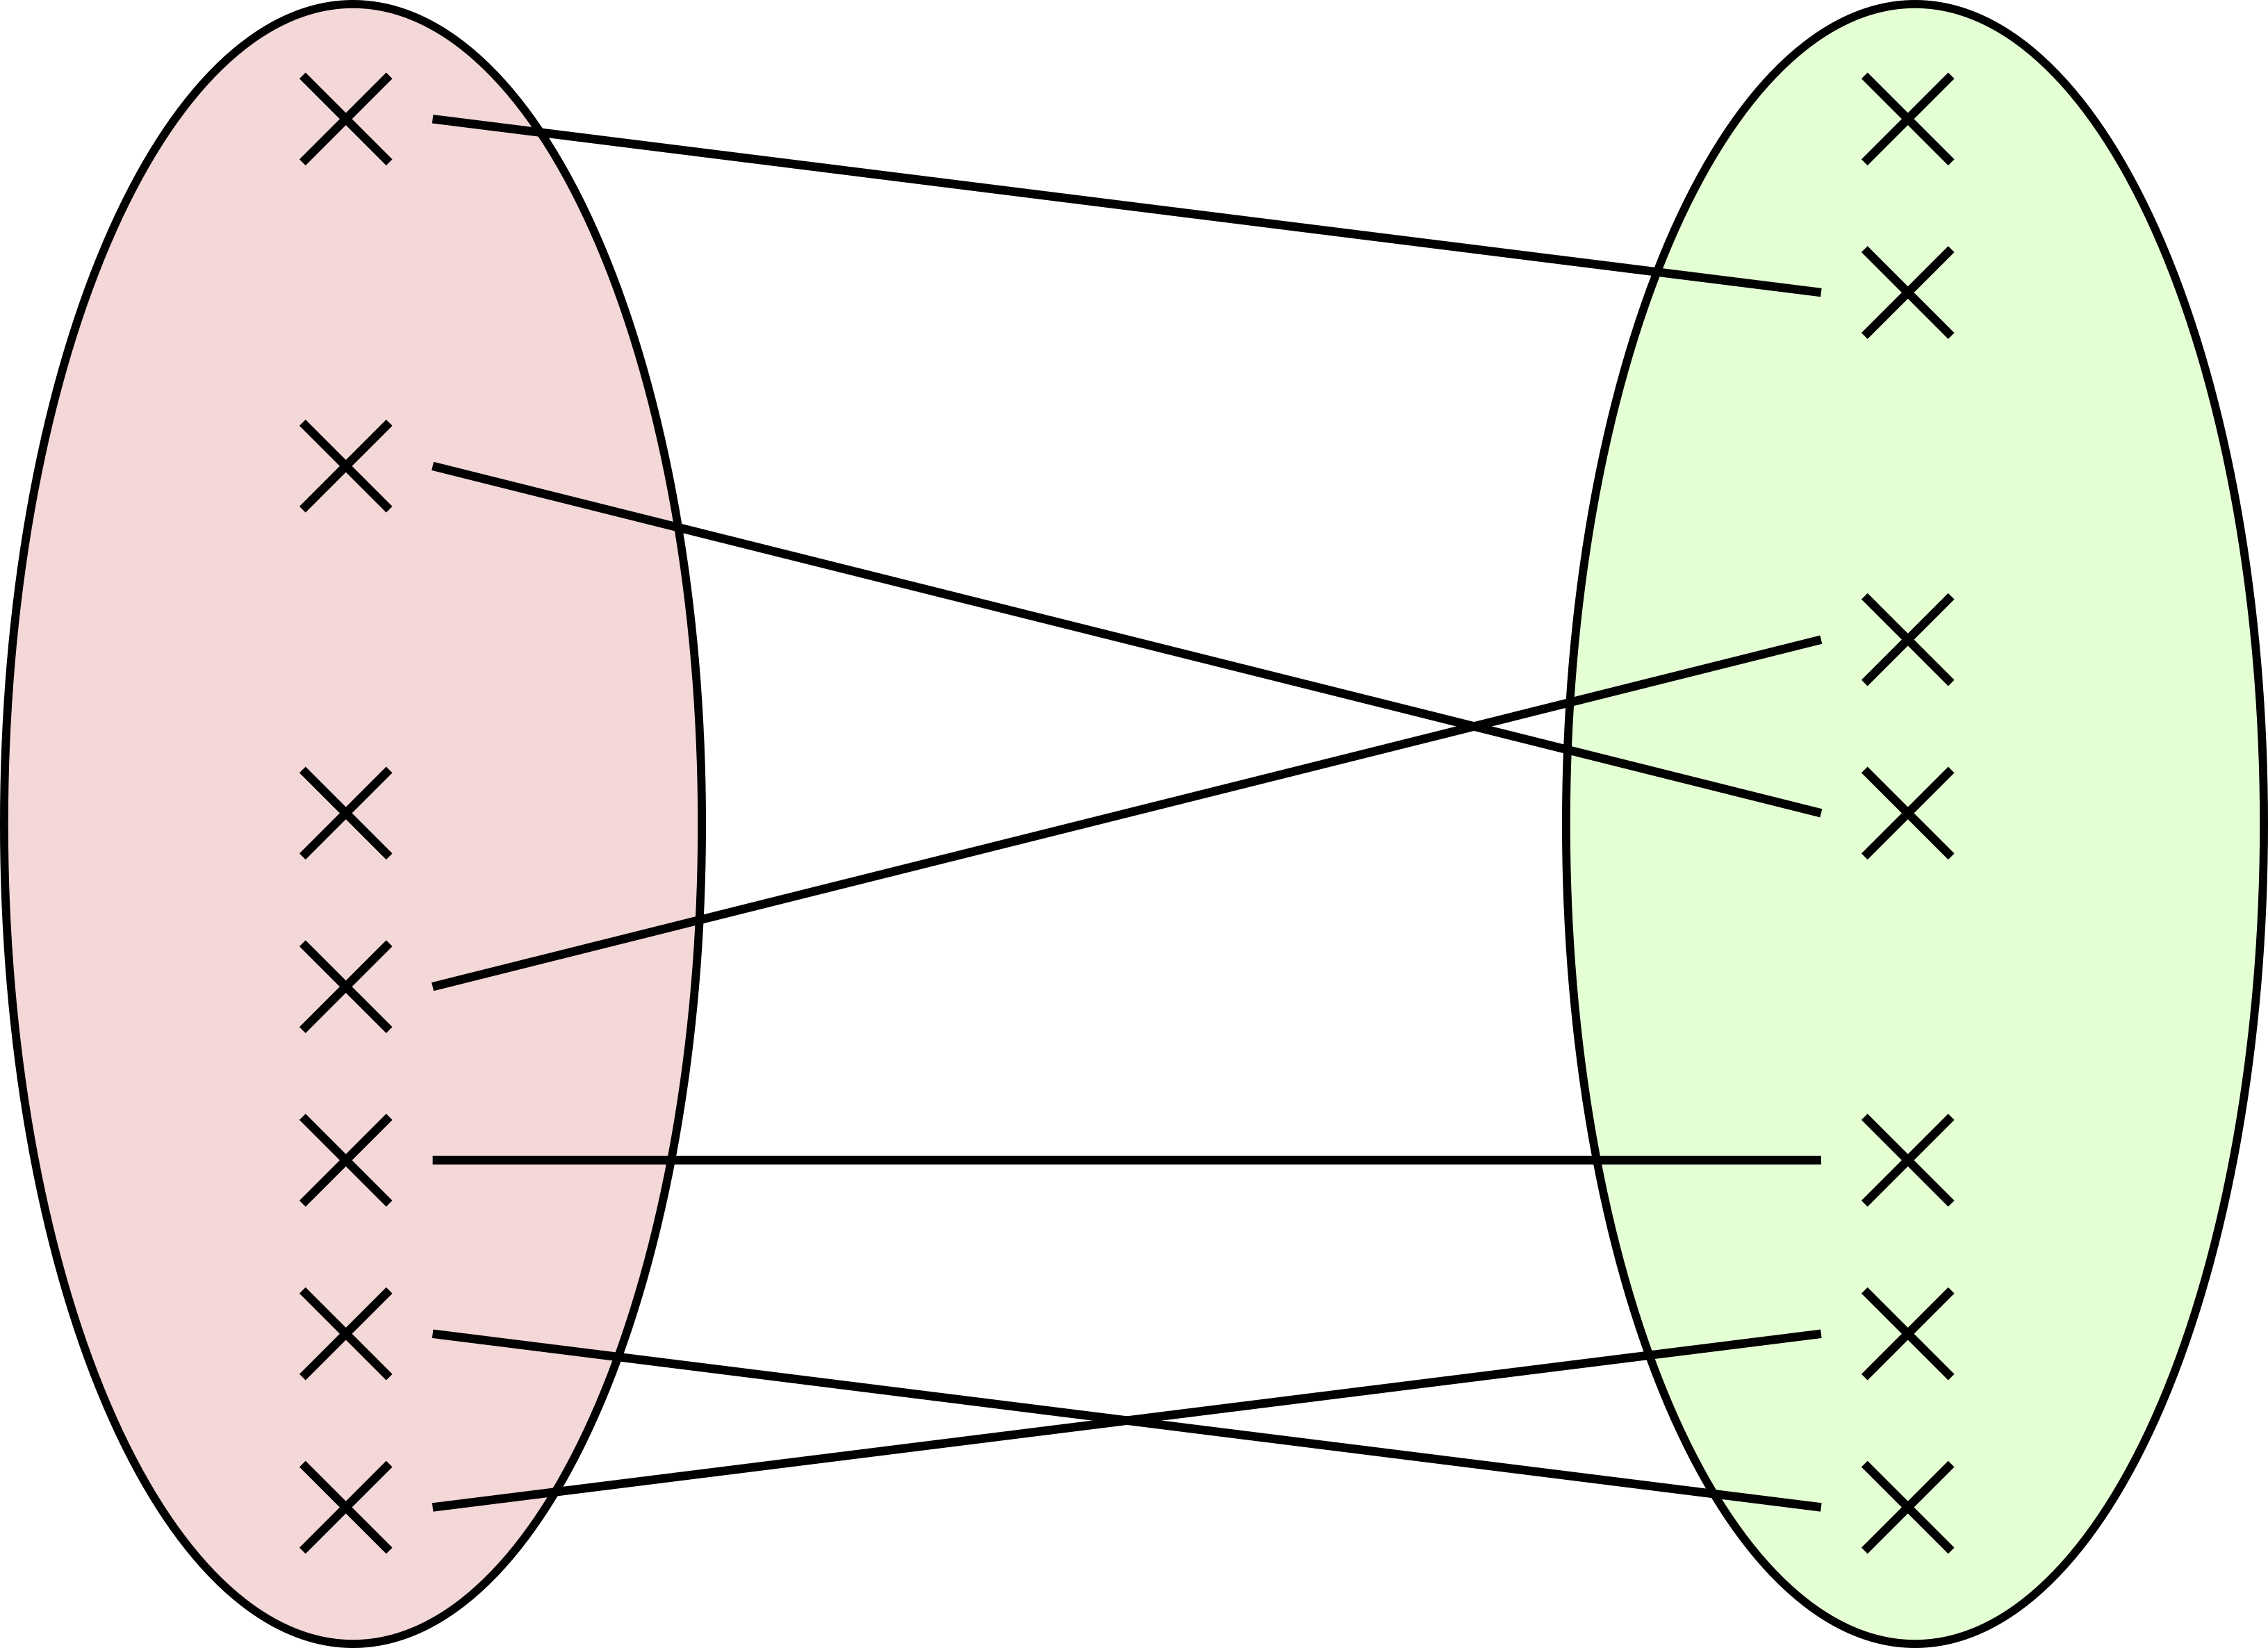
\includegraphics[width=\myw]{ensembles/img/8.png}
        \end{enumerate}    
    \end{multicols}
    
\end{exercice}

\begin{propriete}[ : bijection réciproque]
    Lorsque $f$ est une bijection de $E$ dans $F$, il est possible de construire sa \textit{bijection réciproque}. On la note $f^{-1}$, elle part de $F$, arrive dans $E$ et à tout élément $y$ de $F$ elle associe \textit{son unique antécédent} par $f$.
    \begin{center}
        \begin{tabbing}
            $f^{-1}\,:\,$ \=	$F\longrightarrow E$\\
            \>	$y \longmapsto x$\ \ où $x$ est l'unique élément de $E$ tel que $f(x)=y$.
        \end{tabbing}
    \end{center}
    Et on écrit que $x=f^{-1}(y)$.\\
\end{propriete}

\begin{exemple}[]
    $f$ est une bijection de $E$ dans $F$ : chaque élément de $F$ possède \textit{un unique} antécédent par $f$.\\
    Cela permet de construire la \textit{bijection réciproque} de $f$, notée $f^{-1}$. Celle-ci va de $F$ vers $E$. Puisque $f(e)=r$, on pose alors $f^{-1}(r)=e$, \textit{et c\ae tera}.\\
    \begin{center}
    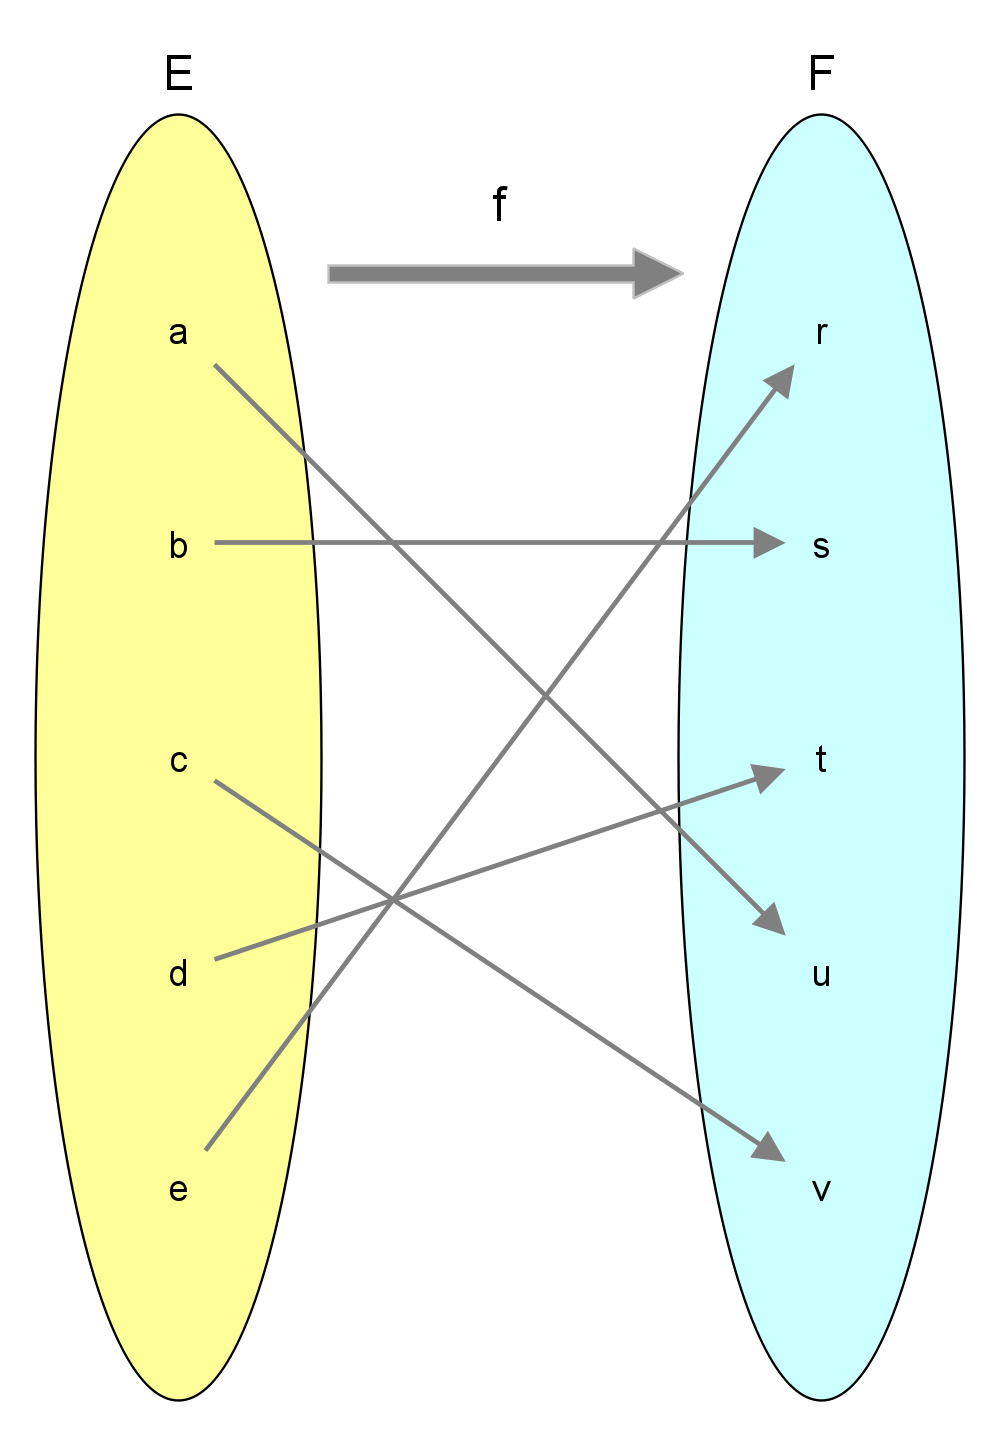
\includegraphics[width=5cm]{ensembles/img/bij.png}\hspace{4em}
    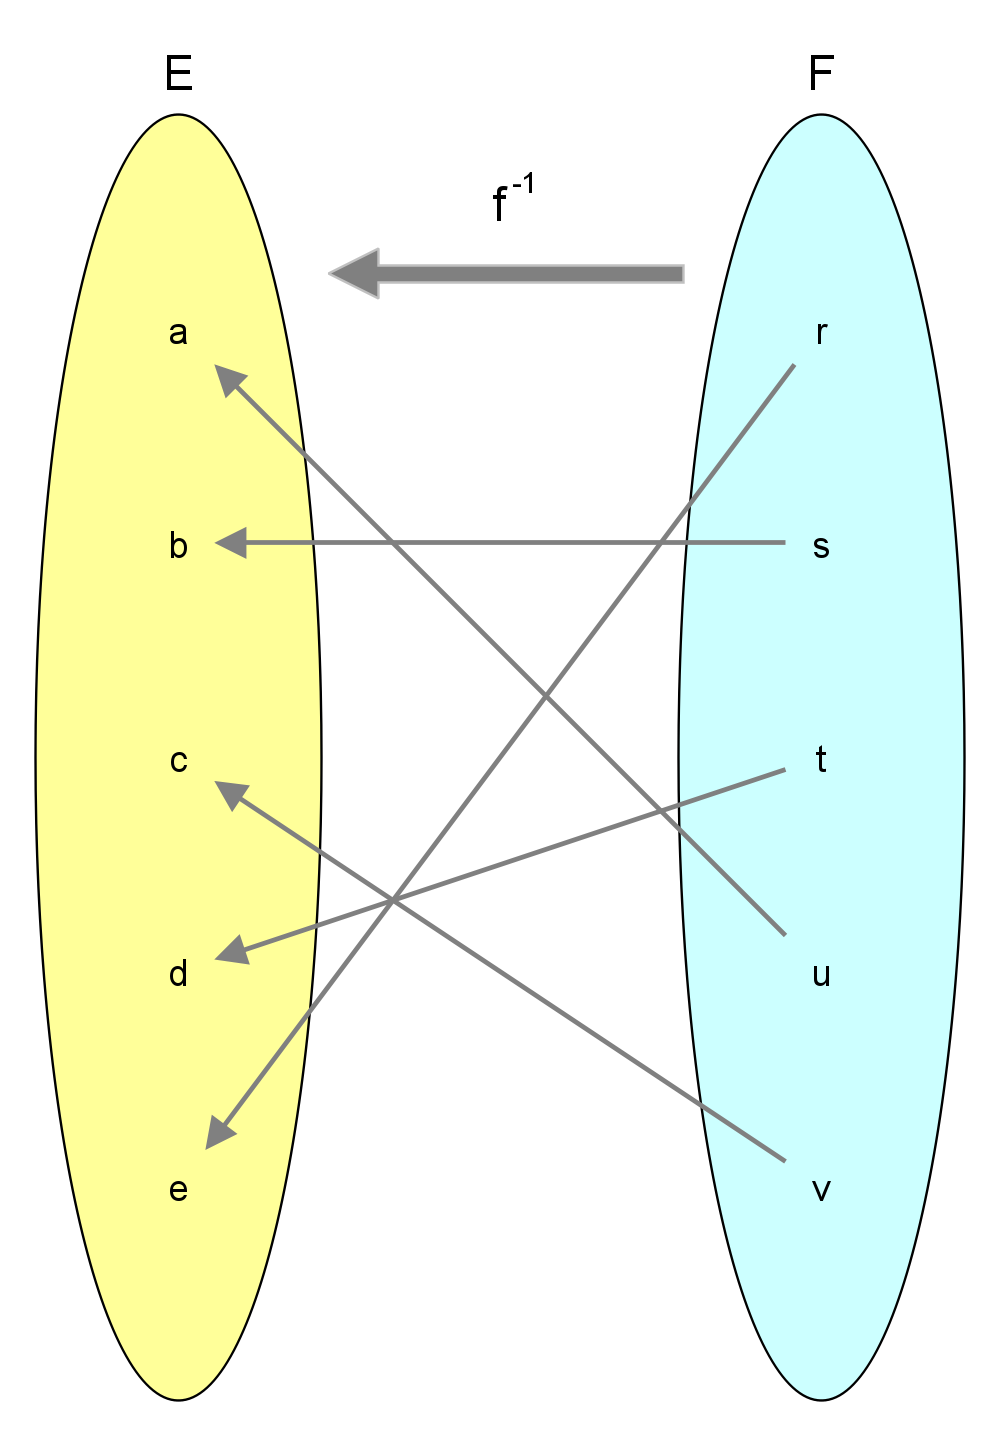
\includegraphics[width=5cm]{ensembles/img/bij_rec.png}
    \end{center}
    Il va sans dire que $f^{-1}$ est également une bijection.
\end{exemple}

\section{Extension aux parties d'une application}

\begin{definition}[ : image directe]
    Soit $f$ une application de $E$ dans $F$ et $A$ une partie de $E$. On appelle \textit{image directe de $A$ par $f$} et on note $f(A)$ la partie de $F$ constituée des images des éléments de $A$ par $f$.
    $$f(A)=\left\lbrace f(x)\::\:x\in A\right\rbrace$$
\end{definition}

\begin{exemple}[]
    $A$ est la partie de $E$ constituée de $a$, $b$, $c$.\\
    On considère $B$, partie de $F$ constituée de $f(a)=s$, $f(b)=r$ et $f(c)=s$ (élément déjà atteint par $a$).$$B=f(A)$$
    \begin{center}
        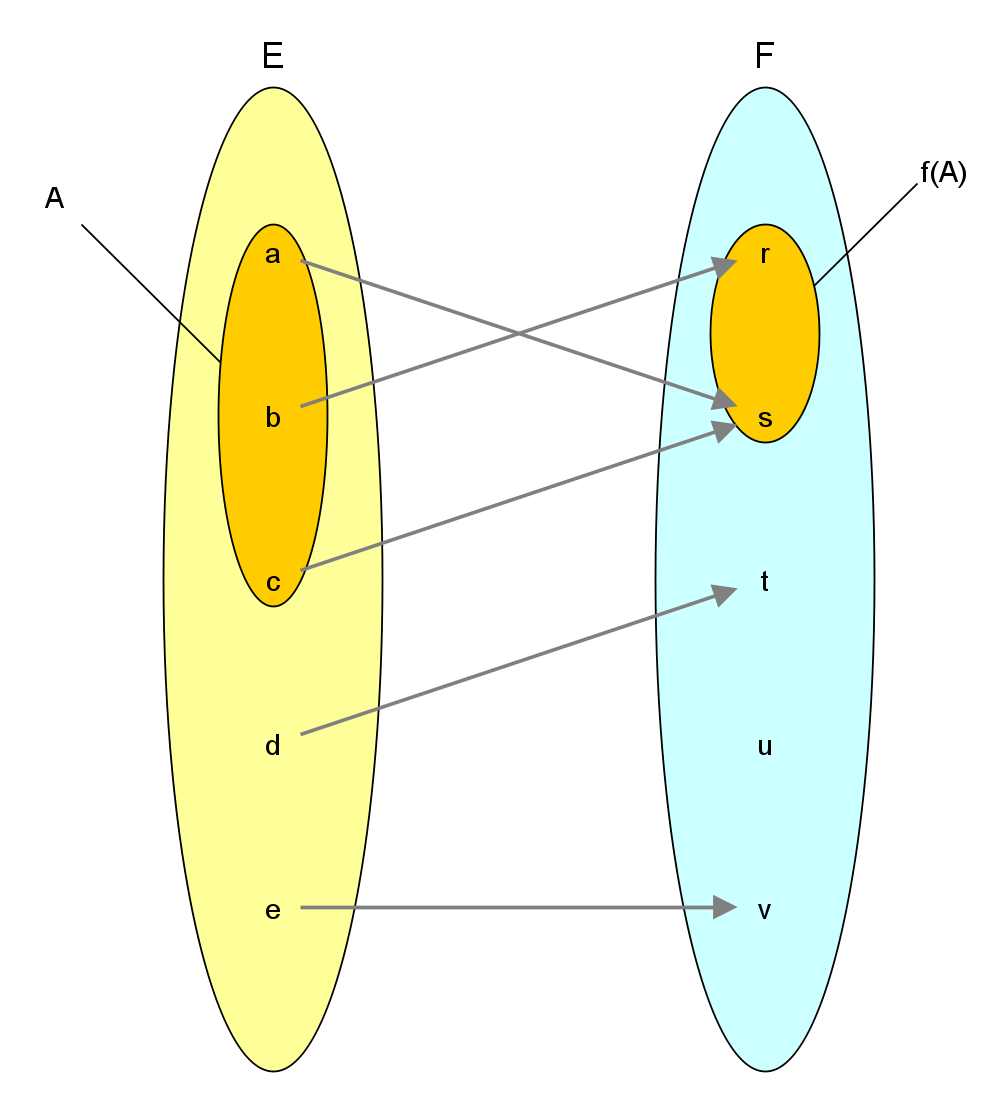
\includegraphics[width=5cm]{ensembles/img/im_dir.png}
    \end{center}
\end{exemple}

\begin{definition}[ : image réciproque]
    Soit $f$ une application de $E$ dans $F$ et $B$ une partie de $F$. On appelle \textit{image réciproque de $B$ par $f$} et on note $f^{-1}(B)$ la partie de $E$ constituée des \textit{antécédents} des éléments de $B$ par $f$.
    $$f^{-1}(B)=\left\lbrace x\in E\::\:f(x)\in B\right\rbrace$$
\end{definition}

\begin{exemple}[]
    \begin{center}
        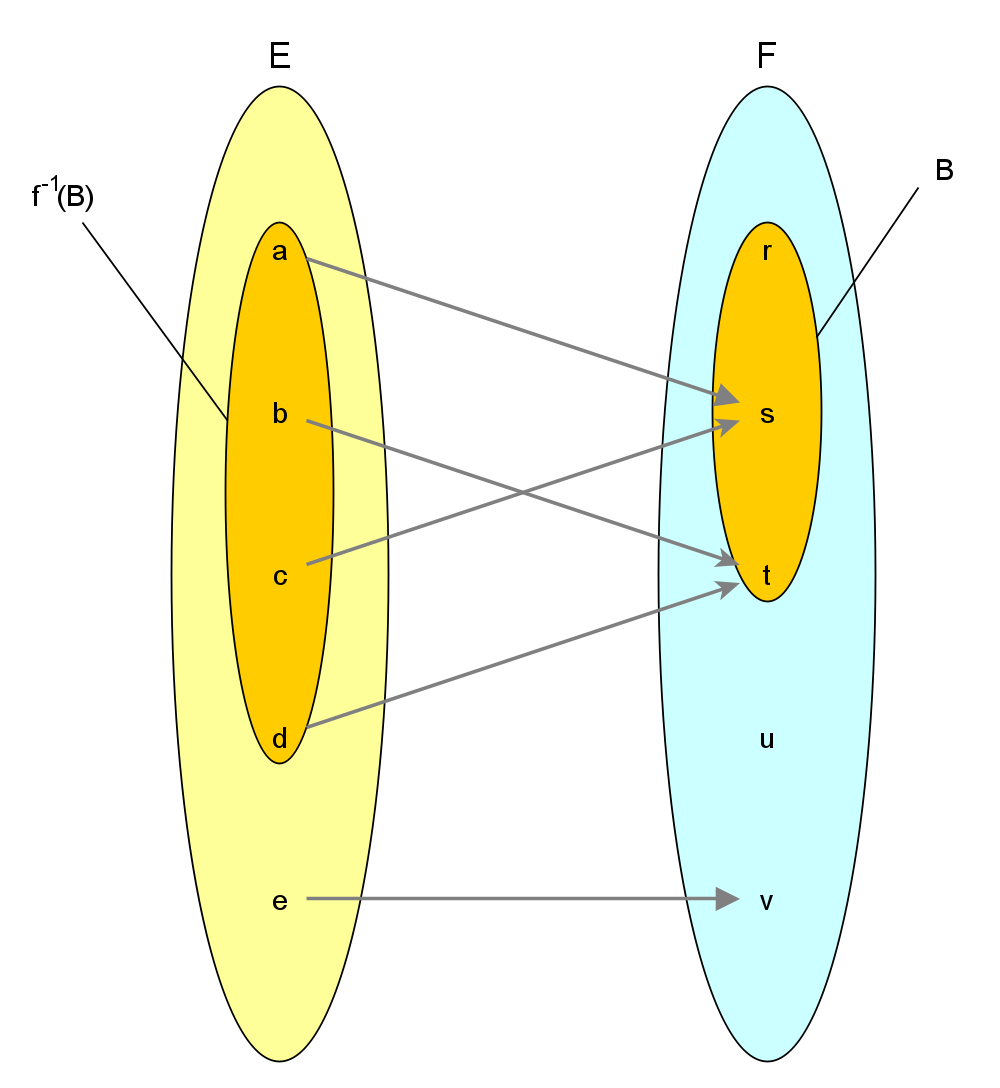
\includegraphics[width=5cm]{ensembles/img/im_rec.png}
    \end{center}
    $B$ est la partie de $F$ constituée de $r$, $s$, $t$.\\
    $r$ n'a pas d'antécédent par $f$, $s$ en a deux : $a$ et $c$, et $t$ en a également 2 : $b$ et $d$.\\
    $$f^{-1}(B)=\left\lbrace a;\,b;\,c;\,d\right\rbrace$$
\end{exemple}

\begin{remarque}[]
    La notation $f^{-1}$ est trompeuse : $f$ n'est pas obligatoirement bijective, donc l'\textit{application} $f^{-1}$ n'est pas obligatoirement définie. Ceci dit il est possible de déterminer $f^{-1}(B)$ quand $B$ est une \textit{partie} de F même si $f$ n'est pas bijective.
\end{remarque}

\begin{exercice}[]
    $E=\lbrace 0;1;2;3;4;5;6;7\rbrace$ et $F=\lbrace 0;1;2;3\rbrace$.\\
    $f$ est l'application de $E$ dans $F$ qui à tout élément de $E$ associe son reste dans la division euclidienne par 3.
    \begin{enumerate}
        \item 	$f$ est-elle injective ? Surjective ?
        \item 	Posons $A=\lbrace 1;3;4\rbrace$, déterminer $f(A)$, puis posant $B=f(A)$, déterminer $f^{-1}(B)$.
        \item 	Posons $C=\lbrace 2;3\rbrace$, déterminer $f^{-1}(C)$, puis, en posant $D=f^{-1}(C)$, déterminer $f(D)$.\\
    \end{enumerate}
\end{exercice}


\begin{exercice}[]
    Soit $f$ l'application de $\R$. dans $\R$. définie par $f(x) = 4x + 10$.
    \begin{enumerate}
        \item 	f est-elle une injection ?
        \item 	f est-elle une surjection ?
        \item 	f est-elle une bijection ?
        \item 	Déterminer l'image directe de $\fif{2}{3}$ et de $\fii{0}$.
        \item 	Déterminer l'image réciproque de $\fii{0}$.\\
    \end{enumerate}
\end{exercice}


\section{Composition}

\begin{definition}[ : composée de deux applications]
    Soit $f$ une application de $E$ dans $F$ et $g$ une application de $F$ dans $G$.\\
    Alors on définit la \textit{composée} de $g$ par $f$ et on note $g\circ f$ l'application de $E$ dans $G$ définie par
    $$g\circ f (x)= g\left(f(x)\right)$$
\end{definition}

\begin{exemple}[]
    Les applications $f$ et $g$ sont décrites par le diagramme ci-contre.\\
    L'application $g\circ f$ est donc définie de $E$ dans $G$ et
    \begin{itemize}
        \item 	$g\circ f(a)=2$
        \item 	$g\circ f(b)=1$
        \item 	$g\circ f(c)=2$
        \item 	$g\circ f(d)=1$
        \item 	$g\circ f(e)=4$
    \end{itemize}
    \begin{center}
        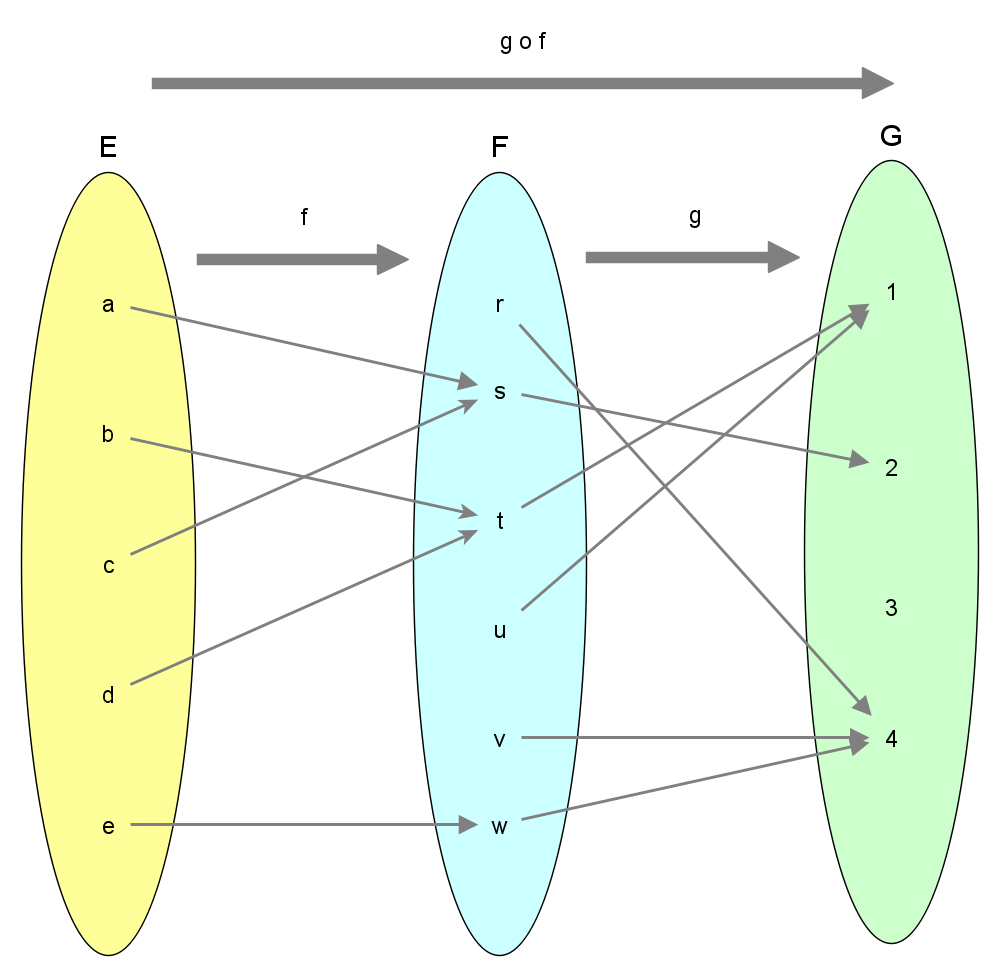
\includegraphics[width=7cm]{ensembles/img/compo.png}
    \end{center}
\end{exemple}

\begin{exercice}[]
    $E=\lbrace a;b;c;d\rbrace$, $F=\lbrace 1;2;3\rbrace$ et $G\lbrace \alpha;\beta;\gamma\rbrace$.\\
    $f$ est définie de $E$ dans $F$  et $g$ de $F$ dans $G$ par\\
    $f(a)=2$, $f(b)=1$, $f(c)=3$ et $g(1)=\gamma$, $g(2)=\alpha$ et $g(3)=\beta$.
    \begin{enumerate}
        \item 	$f$ et $g$ sont-elles injectives ? Surjectives ? Bijectives ?
        \item 	Définir l'application $g\circ f$.
        \item 	Peut-on définir l'application réciproque de $f$ ? De $g$ ?
    \end{enumerate}
\end{exercice}

\begin{exercice}[*]
    Expliciter  $f\circ g$ et $g\circ f$ lorsque $f$ et $g$
    sont les fonctions suivantes :
    \begin{multicols}{2}
        \begin{tabbing}
            $f\ :\ $	\=	$\R$	\=	$\longrightarrow$	\=	$\oii{0}$\\
            \>	$x$		\> 	$\longmapsto$		\>	$x^2+2$
        \end{tabbing}
        \begin{tabbing}
            $g\ :\ $	\=	$\oii{0}$	\=	$\longrightarrow$	\=	$\R$\\
            \>	$x$		\> 	$\longmapsto$		\>	$\dfrac{1}{\sqrt{x}-1}$
        \end{tabbing}
    \end{multicols}
\end{exercice}

\begin{exercice}[]
    Un administrateur réseau gère le parc d'une petite entreprise qui comprend 9 ordinateurs. Chaque
    ordinateur possède une adresse de carte réseau, dite adresse MAC (Media Access Control) unique.\\
    L'administrateur a assigné une adresse IP (Internet Protocol) à chaque ordinateur à l'aide d'un
    logiciel installé sur le serveur. Il obtient le tableau suivant:
    \begin{center}
        \tabstyled
        \begin{tabular}{c|c|c}\hline
            
            \ccell Adresse MAC            & \ccell n° de poste & \ccell Adresse IP \\ \hline
            00~:~FF~:~B4~:~A9~:~96~:~11 & 1                       & 172.16.0.21     \\ \hline
            00~:~FF~:~B4~:~B0~:~45~:~1A & 2                       & 172.16.0.22     \\ \hline
            00~:~FF~:~B4~:~00~:~C5~:~DE & 3                       & 172.16.0.23     \\ \hline
            00~:~EE~:~B5~:~01~:~32~:~C4 & 4                       & 172.16.0.24     \\ \hline
            00~:~EE~:~B5~:~01~:~32~:~C5 & 5                       & 172.16.0.25     \\ \hline
            00~:~EE~:~B5~:~01~:~32~:~C6 & 6                       & 172.16.0.26     \\ \hline
            00~:~FF~:~B4~:~00~:~C5~:~DF & 7                       & 172.16.0.27     \\ \hline
            00~:~FF~:~B4~:~00~:~02~:~98 & 8                       & 172.16.0.28     \\ \hline
            00~:~EE~:~B5~:~01~:~34~:~CA & 9                       & 172.16.0.29     \\ \hline
        \end{tabular}
    \end{center}

    On considère l'application $f$ qui, à un numéro d'ordinateur, associe la dernière partie de l'adresse IP.\\
    Cette dernière partie est un entier variant de 2 à 255.

    %\[f :\: \lbrace 1~;~21~;~31~;~41~;~51~;~61~;~71~;~81~;~9\rbrace  \longto  \lbrace 21~;~31~;~\ldots1~;~255\rbrace .\]

    \[f :\: \left\lbrace 1~;~2~;~3~;~4~;~5~;~6~;~7~;~8~;~9 \rule{0pt}{9pt}\right\rbrace \longrightarrow \left\lbrace 2~;~3~;~\ldots~;~255\rule{0pt}{9pt}\right\rbrace.\]
    Par exemple, $f(1) = 21$.
    \begin{enumerate}
        \item Justifier le fait que cette application est injective.
        \item Cette application est-elle surjective ? Justifier.
        \item À la suite d'une opération informatique, le poste dont l'adresse MAC est

              00~:~FF~:~B4~:~00~:~C5~:~DF obtient l'adresse IP suivante : 172.16.0.23. Les autres postes gardent leur adresse IP précédente.

              On a alors une nouvelle application

              %$g : \:\lbrace 11~;~21~;~31~;~41~;~51~;~61~;~71~;~81~;~9\rbrace  \longmapsto \lbrace 21~;~31~;~\ldots1~;~255\rbrace$.

              \[g : \:\left\lbrace 1~;~2~;~3~;~4~;~5~;~6~;~7~;~8~;~9\rule{0pt}{9pt}\right\rbrace \longrightarrow\left\lbrace 2~;~3~;~\ldots~;~255\rule{0pt}{9pt}\right\rbrace.\]

              L'application $g$  est-elle injective ? Justifier.
    \end{enumerate}
\end{exercice}